%% 
%% Copyright 2019-2024 Elsevier Ltd
%% 
%% Version 2.4
%% 
%% This file is part of the 'CAS Bundle'.
%% --------------------------------------
%% 
%% It may be distributed under the conditions of the LaTeX Project Public
%% License, either version 1.2 of this license or (at your option) any
%% later version.  The latest version of this license is in
%%    http://www.latex-project.org/lppl.txt
%% and version 1.2 or later is part of all distributions of LaTeX
%% version 1999/12/01 or later.
%% 
%% The list of all files belonging to the 'CAS Bundle' is
%% given in the file `manifest.txt'.
%% 
%% Template article for cas-sc documentclass for 
%% single column output.

%\documentclass[a4paper,fleqn,longmktitle]{cas-sc}
\documentclass[a4paper,fleqn]{cas-sc}

%\usepackage[numbers]{natbib}
%\usepackage[authoryear]{natbib}
\usepackage[authoryear]{natbib}
\usepackage[utf8]{inputenc}
\usepackage[T1]{fontenc}    % Fixed hidden spaces here
\usepackage{hyperref}       % Fixed hidden spaces here
\usepackage{url}
\usepackage{booktabs}
\usepackage{amsfonts}
\usepackage{nicefrac}
\usepackage{microtype}
\usepackage{lipsum}
\usepackage{graphicx}
\usepackage{natbib}
\usepackage{doi}
\usepackage{tabularx}
\usepackage{multirow}
\usepackage{diagbox}
\usepackage{array}          % ADDED: Required for your table alignments
\usepackage{amsmath}
\usepackage{cleveref}       %
\usepackage{algorithm}
\usepackage{algorithmic}
\usepackage{booktabs}
\usepackage{placeins}
\usepackage{float}
\usepackage{xcolor}

% LaTeX command names may contain letters only (\rev1 is not a valid name)
\newcommand{\revone}[1]{\textcolor{red}{#1}}   % Reviewer 1
\newcommand{\revtwo}[1]{\textcolor{blue}{#1}}  % Reviewer 2
\definecolor{revgreen}{RGB}{0,100,0}  % dark green, readable on white
\newcommand{\revthree}[1]{\textcolor{revgreen}{#1}} % Reviewer 4
\definecolor{revshared}{RGB}{128,0,160} % purple, comments shared by several reviewers
% Optional argument lists the reviewers (e.g. \revcommon[R1,R4]{...}); it is not printed
\DeclareRobustCommand{\revcommon}[2][]{\textcolor{revshared}{#2}} % Common reviewer comments

\hypersetup{
    colorlinks=true,
    citecolor=blue,
    linkcolor=blue,
    urlcolor=blue
}
%%%Author macros
\def\tsc#1{\csdef{#1}{\textsc{\lowercase{#1}}\xspace}}
\tsc{WGM}
\tsc{QE}
\tsc{EP}
\tsc{PMS}
\tsc{BEC}
\tsc{DE}
%%%

\begin{document}
\let\WriteBookmarks\relax
\def\floatpagepagefraction{1}
\def\textpagefraction{.001}
% \shorttitle{Leveraging social media news}
% \shortauthors{J.K. Krishnan et~al.}
%\begin{frontmatter}

\title [mode = title]{Diverse Initializations for Vector Ensembles in Representation-aware Text-Attributed Graph Encoding with Large Language Models}   
\shorttitle{Diverse Initializations for Vector Ensembles in Representation-aware TAG Encoding with LLMs}                   
% \tnotemark[1,2]

% \tnotetext[1]{This document is the results of the research
%    project funded by the National Science Foundation.}

% \tnotetext[2]{The second title footnote which is a longer text matter
%    to fill through the whole text width and overflow into
%    another line in the footnotes area of the first page.}




% \cormark[2]
% \fnmark[1,3]
% \ead{t.rafeeq@example.in}
% \ead[URL]{www.campus.in}

% \cortext[cor1]{Corresponding author}
% \cortext[cor2]{Principal corresponding author}
% \fntext[fn1]{This is the first author footnote, but is common to third
%   author as well.}
% \fntext[fn2]{Another author footnote, this is a very long footnote and
%   it should be a really long footnote. But this footnote is not yet
%   sufficiently long enough to make two lines of footnote text.}

% \nonumnote{This note has no numbers. In this work we demonstrate $a_b$
%   the formation Y\_1 of a new type of polariton on the interface
%   between a cuprous oxide slab and a polystyrene micro-sphere placed
%   on the slab.
%   }

\begin{abstract}
Learning on text-attributed graphs requires combining rich node text with graph structure, but existing LLM--GNN methods often depend on expensive textual augmentation, external APIs, or a single fine-tuned encoder whose representations may be brittle for downstream graph learning.
This study addresses how to obtain diverse, high-quality text-derived node representations and combine them effectively for node classification without augmenting node text. We introduce DIVERGE, which repeatedly fine-tunes one LLM on native node texts and labels using diverse LoRA initializations, trains a GNN on each resulting embedding set, and adaptively ensembles the GNN pool with trainable model- and class-level weights.
\revcommon[R1,R2,R4]{On seven benchmarks from five domains (citation, biomedical, Wikipedia, social-media and e-commerce graphs), with all baselines except two LLM predictors re-run under the same splits and seeds, DIVERGE achieved the best accuracy on six benchmarks and the best Macro-F1 on all seven; on Reddit, a 7B instruction-tuned predictor was more accurate unless DIVERGE used a GCN backbone. The gains held for three LLM encoders and three GNN architectures, and two or three views already captured most of them. Controlled experiments showed that the initialization adds diversity beyond training randomness and is a larger source of diversity than the random seed, most clearly in weight space. The learned ensemble weights were more accurate than uniform averaging in every encoder--dataset pair, with the largest gains where one view's fine-tuning collapsed.} These findings show that representation diversity induced from native graph text can match or exceed augmentation-based approaches \revone{without any external API calls, at the price of additional local GPU time}. Because all encoding runs on locally fine-tuned models without transmitting node text to third-party services, DIVERGE is also well suited to privacy-sensitive settings such as institutional repositories, enterprise document networks, and regulated biomedical corpora\revone{, provided that the saved embeddings and adapters, which still reveal parts of the text, are protected like the raw data}.
\end{abstract}

% \begin{graphicalabstract}
% \includegraphics{figs/cas-grabs.pdf}
% \end{graphicalabstract}

% \begin{highlights}
% \item Research highlights item 1
% \item Research highlights item 2
% \item Research highlights item 3
% \end{highlights}

\begin{keywords}
Text-Attributed Graphs \sep
Large Language Models \sep
Graph Neural Networks \sep
Ensemble Learning \sep
LLM on Graph \sep
Parameter-efficient fine-tuning \sep
Data privacy

\end{keywords}


\maketitle

\section{Introduction}

\textbf{Text-attributed graphs (TAGs)} model entities and their relationships through both network structure and associated text, appearing in social networks, citation graphs, and e-commerce platforms \citep{zhang2025leveraging, he2024harnessing}. \textbf{Graph neural networks (GNNs)} have traditionally processed these graphs using shallow embeddings or fine-tuned language models such as BERT \citep{devlin2018bert}. However, such encoders often fail to capture the semantic depth and world knowledge required for accurate node classification \citep{he2024harnessing, zhang2025leveraging}.

\textbf{Large language models (LLMs)}, including GPT and LLaMA, offer stronger contextual understanding and have motivated a new generation of LLM--GNN methods \citep{brown2020language, touvron2023llama}. Integrating LLMs with graphs nevertheless remains challenging because API-based annotation scales poorly to millions of nodes, exposes proprietary or sensitive node text to third-party cloud providers, and because LLM-generated features can introduce noise, hallucinations, and inference-time distribution shift \citep{Jaiswal2024AllAgainstSome, hu2025gaga, zhang2025leveraging}.


Recent research studies have addressed these hurdles through several innovative strategies:
\begin{itemize}
    \item \textbf{Explanations as Features:} Approaches such as \textbf{TAPE} leverage the reasoning abilities of LLMs by using their decision-making explanations as vectorial node features, which significantly boosts GNN performance without requiring full LLM fine-tuning  \citep{he2024harnessing}.
    \item \textbf{Efficient Integration and Inference:} Frameworks like \textbf{E-LLaGNN} utilize LLMs as an on-demand service to enhance only a tactical fraction of nodes, thereby reducing the computational footprint and facilitating \textbf{LLM-free inference} for industrial deployment  \citep{Jaiswal2024AllAgainstSome}.
    \item \textbf{Topological Structure Refinement:} Models like \textbf{GraphEdit} and \textbf{GAGA} employ LLMs to learn complex node relationships globally, effectively denoising connections by removing unreliable edges and adding reliable ones based on semantic similarity  \citep{guo2024graphedit, li2024gaga, Sun2026TopologicalEnhancerTAG}.
    \item \textbf{Cost-Effective Labeling:} New active self-training frameworks, such as \textbf{Locle}, identify "critical" samples for LLM annotation while utilizing GNN-based graph rewiring to refine labels, achieving state-of-the-art results for \textbf{label-free node classification} at a minimal cost  \citep{zhang2025leveraging}.
\end{itemize}

Despite this progress, three limitations motivate our work. First, augmentation-heavy pipelines such as TAPE \citep{he2024harnessing} depend on external LLM APIs and can hurt accuracy when node texts are already informative (Section~\ref{sec:Preliminaries}). Second, sending full node corpora to remote APIs creates privacy, retention, and compliance risks in institutional, enterprise, and regulated domains where graph text must remain on premises. Third, existing ensemble variants typically average GNN logits uniformly, which cannot exploit class-specific strengths of different representations. We therefore propose \textbf{DIVERGE}, a framework that induces diverse semantic views through multiple LoRA initializations and combines the resulting GNNs with adaptive, trainable weighting---without textual augmentation, paid API calls, or off-site disclosure of node text.


From an \textbf{information-processing perspective}, TAG node classification supports core tasks in bibliometrics, digital libraries, knowledge-base curation, knowledge graph and recommendation over linked documents \citep{Zhang2024TAGSurvey, RAMIREZMOLINA2026104842, WANG2026DGRLS}. Citation and hyperlink graphs encode how scientific ideas, web pages, and catalogued entities relate to one another; accurate categorization of nodes directly affects literature discovery, expert finding, and knowledge-network maintenance.

Our main contributions are as follows:
\begin{itemize}
	\item We propose \textbf{DIVERGE}, a novel framework for text-attributed graph learning that generates diverse semantic representations using multiple parameter-efficient LLM fine-tuning processes with different LoRA initialization strategies, without requiring textual augmentation or external LLM API calls.
	
	\item We introduce an adaptive ensemble learning framework that combines multiple GNNs trained on heterogeneous textual representations using trainable weighting mechanisms, including model-level and class-level aggregation strategies.
	
	\item We demonstrate that diverse representations can be effectively induced solely from the original graph texts and graph structure, eliminating the need for costly LLM-generated augmented texts \revone{and the API fees they require (in exchange for additional local GPU time; Section~\ref{sec:efficiency})}, and keeping all node text within the operator's trusted infrastructure---an important requirement for privacy-sensitive and compliance-constrained deployments.
\item We highlight a practical advantage of local, API-free encoding: DIVERGE never transmits proprietary node descriptions to external LLM services, which supports on-premises deployment in bibliographic systems, enterprise knowledge graphs, and regulated biomedical corpora where data residency and confidentiality constraints prohibit cloud-based augmentation\revone{; we also measure how much text still leaks through the saved embeddings and state what local deployment does not protect against (Section~\ref{sec:privacy})}.
	
	\item \revcommon[R1,R2,R4]{Experiments on seven TAG benchmarks from five domains (Cora, CiteSeer, PubMed, WikiCS, OGBN-ArXiv, Reddit and Computers), with three LLM encoders, three GNN encoders and four random splits, and with the baselines re-run under the same protocol, show that DIVERGE achieves the best accuracy on six benchmarks and the best Macro-F1 on all seven.}

	\item \revcommon[R1,R2,R4]{Through controlled seed-versus-initialization experiments, we show that the LoRA initialization places each adapter in a distinct and stable region of the weight space, that this difference propagates to the embeddings and predictions, and that the initialization adds diversity beyond training randomness. We further show that the softmax-constrained ensemble weights match uniform averaging when the views are balanced and clearly improve over it when one view is weak.}
\end{itemize}

The structure of the paper is as follows: in Section~\ref{sec:relatedWork}, we review existing studies on integrating LLMs and GNNs for text-attributed graphs. Section~\ref{sec:Preliminaries} presents the motivation and preliminaries of the proposed framework. In Section~\ref{sec:Methodology}, the proposed DIVERGE methodology is described in detail, including the diverse LoRA initialization strategies, representation extraction process, and adaptive ensemble learning mechanisms. Section~\ref{sec:Evaluation} introduces the datasets, baselines, implementation details, and evaluation metrics used in the experiments. Section~\ref{sec:Results} reports the experimental results and ablation studies. Section~\ref{sec:Discussion} interprets these findings, articulates their theoretical and practical implications, and positions DIVERGE relative to prior work. Section~\ref{sec:Limitations} discusses the limitations of the proposed approach, and Section~\ref{sec:Conclusion} concludes the paper and outlines directions for future work.


\section{Research Objectives}\label{sec:researchObjectives}
Motivated by the limitations of augmentation-heavy LLM--GNN pipelines, this study addresses the following objectives:
\begin{enumerate}
    \item To induce diverse, complementary node representations from native graph texts using multiple LoRA initialization strategies, without textual augmentation, paid LLM APIs, or off-site exposure of sensitive node text.
    \item To design adaptive ensemble mechanisms that weight heterogeneous GNN outputs at model and class levels.
    \item To evaluate DIVERGE against GNN, encoder-, enhancer-, and predictor-based LLM--GNN baselines on \revone{seven TAG benchmarks from five domains, with three LLM encoders and three GNN encoders}.
    \item To analyze when diversity-driven encoding outperforms augmentation-based approaches and quantify gains statistically.
\end{enumerate}

\section{Related Works}\label{sec:relatedWork}
LLMs have recently been integrated with GNNs for processing TAGs. Based on existing studies, We categorize the role of LLMs into three main paradigms: Encoder, Enhancer, and Predictor \citep{Wu2025LLMNode, Jin2023LLMGraphs, Chen2024LLMGraphs, Li2024GraphLLMSurvey}.

\subsection{LLMs as Encoders}
The \textbf{Encoder} paradigm uses LLMs to map node text to vector representations that downstream GNNs consume \citep{he2024harnessing, Huang2024GNNAdapters, Zhu2024EfficientTextualGraphs}. Early pipelines relied on shallow features (bag-of-words, skip-gram); recent methods employ pre-trained LMs or LLMs as text encoders. \textbf{ENGINE} \citep{Zhu2024EfficientTextualGraphs} optimizes end-to-end efficiency for large TAGs through parameter-efficient LLM tuning. \textbf{GraphAdapter} \citep{Huang2024GNNAdapters} injects structural signals into frozen LLMs via lightweight adapters \citep{Houlsby2019Adapters}. \textbf{WalkLM} \citep{Tan2023WalkLM} textualizes random walks to joint learning of text and topology, while \textbf{One-for-All (OFA)} \citep{liu2024oneforall} seeks a unified semantic space across graph domains. \textbf{LEADING} \citep{Xue2025LEADING} further reduces label demand through neighbor decoupling during end-to-end LM--GNN training. \textbf{STAGE} \citep{zolnai-lucas-etal-2024-stage} demonstrates that frozen LLM embeddings combined with ensemble GNN training can be competitive on academic TAGs with minimal pipeline complexity.

\citet{Wu2025LLMNode} release \textbf{LLMNodeBed} and systematically ask \emph{when} LLMs help node classification. Their analysis shows that (a)~encoder-style LLM features consistently outperform bag-of-words and shallow LM baselines on most TAG benchmarks, (b)~enhancement-heavy pipelines do not always justify their cost, and (c)~predictor-style LLM methods are sensitive to prompting and scale. These findings motivate DIVERGE's focus on strong \emph{local} encoders rather than paid API augmentation.\textbf{LLM-BP} \citep{wang2025llmbp} proposes task-adaptive LLM embeddings and belief-propagation-style aggregation, improving cross-graph generalization on 11 TAG datasets. DIVERGE differs from LLM-BP by inducing diversity through multiple LoRA initializations of a \emph{single} backbone rather than task-adaptive prompting, and by learning ensemble weights over GNN logits rather than propagating beliefs on a single embedding space.

\subsection{LLMs as Enhancers}
Enhancer methods modify node text, graph structure, or labels before or during GNN training. \textbf{TAPE} \citep{he2024harnessing} generates LLM explanations and zero-shot predictions to enrich node text, then trains multiple GNNs whose logits are \emph{uniformly averaged}. Although effective on several benchmarks, TAPE requires external LLM API access and can introduce semantic noise when native texts are already informative (Section~\ref{sec:Preliminaries}). Structural enhancers include \textbf{RoSE} \citep{Sun2026TopologicalEnhancerTAG} and \textbf{GraphEdit} \citep{guo2024graphedit}. \textbf{LLM4NG} \citep{Yu2025NodeGenerationTAG} synthesizes nodes and edges for few-shot TAG learning.

A second enhancer thread targets \textbf{cost and label efficiency}. \textbf{E-LLaGNN} \citep{Jaiswal2024AllAgainstSome} enhances only critical nodes to enable LLM-free inference at deployment. \textbf{Locle} \citep{zhang2025leveraging} combines active LLM labeling with GNN-based graph rewiring for label-scarce node classification. \textbf{GAGA} \citep{hu2025gaga} annotates representative nodes and aligns an annotation graph with the TAG, requiring as little as 1\% labeled data in reported experiments. \textbf{UltraTAG} \citep{yu2025ultratag} modularizes augmentation, text encoding, and training into a unified robust pipeline (with extensions such as UltraTAG-S for sparse text/edges). \textbf{SKETCH} \citep{zhou-etal-2025sketch} decouples semantic and structural aggregation: it retrieves related node texts and distant structural contexts before long-context LM training, reducing reliance on conventional GNN propagation while improving efficiency.

Collectively, enhancer methods demonstrate that LLMs can improve TAG learning by enriching inputs---but often at the cost of API fees, hallucination risk, or complex multi-stage pipelines. DIVERGE deliberately avoids textual augmentation and instead asks whether comparable gains can arise from \emph{diverse encodings of native text}.

\subsection{LLMs as Predictor}
In the \textbf{Predictor} paradigm, LLMs directly perform reasoning tasks on text-attributed graphs. Methods like \textbf{GRAPHTEXT} transform graph structures into "Graph-Syntax Trees" that are flattened into textual sequences, allowing LLMs to reason over the graph as a text-generation task \citep{Zhao2024GraphText}. Other approaches adapt LLMs to better capture structural knowledge by mapping graphs into ordered node sequences or injecting structural embeddings into the LLM's input space using projectors or prefix tuning, as seen in \textbf{DGTL} \citep{Qin2024DisentangledTAG} and \textbf{LLaGA} \citet{Chen2024LLaGA}. Additionally, the \textbf{ZeroG} framework explores cross-dataset zero-shot transferability, leveraging a shared semantic space to apply graph knowledge without task-specific fine-tuning \citep{Li2024ZeroG}.These methods lie outside our encoder–GNN
design and are included only as baselines in Section \ref{sec:Evaluation}.

\subsection{Ensemble learning and representation diversity}

Ensembling multiple graph learners is not new, but \emph{how} models are combined varies widely. TAPE averages GNN logits with fixed equal weights \citep{he2024harnessing}. STAGE and LLMNodeBed benchmarks show that even simple encoder ensembles can be strong \citep{zolnai-lucas-etal-2024-stage, Wu2025LLMNode}. LLM-BP advances aggregation through learned, graph-adaptive belief propagation \citep{wang2025llmbp}. Yet most LLM--GNN pipelines still derive diversity from \emph{different modalities or pipeline stages} (e.g., augmented vs.\ original text, LM vs.\ GNN), not from multiple parameter-efficient trajectories of the same encoder.

In parallel, parameter-efficient fine-tuning (PEFT) research shows that initialization and low-rank adaptation strategy affect the semantic subspace an LM converges to \citep{Hu2021LoRA, meng2024pissa, paischer2024eva, li2023loftq, zhang2025orthogonal, wang2025peft}. DIVERGE extends this insight to TAGs: we treat \textbf{LoRA initialization diversity} as a controllable source of complementary node representations and combine the resulting GNNs with \textbf{learned} model- and class-level weights rather than uniform averaging.

\subsection{Research gap and position of DIVERGE}

\begin{table}[htbp]
\centering
\caption{Comparison of DIVERGE with representative recent TAG methods (2024--2025).}
\label{tab:related_gap}
\small
\begin{tabular*}{\linewidth}{@{\extracolsep{\fill}} lcccc @{}}
\toprule
\textbf{Method} & \textbf{Augment.\ text?} & \textbf{External API?} & \textbf{Diversity source} & \textbf{Aggregation} \\
\midrule
TAPE \citep{he2024harnessing} & Yes & Yes & Multi-feature/GNN pool & Uniform average \\
UltraTAG \citep{yu2025ultratag} & Yes (module) & Optional & Pipeline modules & Task-specific \\
LLM-BP \citep{wang2025llmbp} & No & Optional & Task-adaptive encoder & Belief propagation \\
SKETCH \citep{zhou-etal-2025sketch} & No (retrieval) & No & Retrieved contexts & LM-centric \\
STAGE \citep{zolnai-lucas-etal-2024-stage} & No & No & Frozen LLM & Ensemble GNN \\
\textbf{DIVERGE (ours)} & \textbf{No} & \textbf{No} & \textbf{Multi-init LoRA} & \textbf{Learned ensemble} \\
\bottomrule
\end{tabular*}
\end{table}

Table~\ref{tab:related_gap} summarizes how DIVERGE relates to representative recent methods. No prior TAG approach simultaneously (1)~induces representation diversity through \textbf{multi-initialization LoRA} on native node text, (2)~trains a \textbf{pool of GNNs} on complementary embeddings, and (3)~fuses predictions with \textbf{learned ensemble weights}---all \textbf{without} LLM-based textual augmentation or external API calls. Methods such as TAPE and UltraTAG rely on augmentation; LLM-BP and SKETCH introduce diversity through task-adaptive prompting or retrieval;STAGE use a single encoding trajectory. DIVERGE fills this gap by showing that initialization-driven diversity plus adaptive ensembling can match or exceed augmentation-based performance (Section~\ref{sec:resultsAnalysis}) while remaining deployable in privacy-sensitive information systems (Section~\ref{sec:Discussion}).


\section{Preliminaries}\label{sec:Preliminaries}
\subsection{Motivation}

Recent studies on TAGs have shown that the quality and richness of node-associated texts play a critical role in the final performance of graph learning models \citep{he2024harnessing}. In citation networks and scientific document graphs, node texts often already contain highly informative semantic content that can strongly support downstream node classification tasks. Consequently, the effectiveness of graph representation learning increasingly depends on how efficiently this semantic information is extracted and utilized.

LLMs have recently emerged as powerful semantic encoders due to their strong contextual understanding and extensive linguistic knowledge. Several recent methods utilize LLMs to augment node texts by generating explanations, summaries, or pseudo-label descriptions for graph nodes \citep{he2024harnessing}. The underlying assumption of these approaches is that additional generated textual information can enrich node semantics and improve graph learning performance.



\begin{table}[h]
\caption{Accuracy of GNNs using different initial node features on the Cora dataset.}
\label{tab:gnn_features_comparison}

\begin{tabular*}{\linewidth}{@{\extracolsep{\fill}} lc @{}}
\toprule
\textbf{Type of Initial Node Features} & \textbf{Accuracy (\%)} \\
\midrule
Embeddings of original graph node texts & 89.14 \\
Embeddings of texts augmented by LLMs (zero-shot prediction) & 87.77 \\
Bag-of-words features & 85.34 \\
\bottomrule
\end{tabular*}
\end{table}

However, experimental observations reveal that textual augmentation is not always beneficial, particularly in graphs whose original node texts are already rich and informative. In such scenarios, generated texts may introduce semantic noise, hallucinated information, or incorrect predictions, which can ultimately degrade downstream graph performance. Table \ref{tab:gnn_features_comparison} demonstrates this phenomenon on the Cora dataset, where embeddings extracted directly from the original graph texts outperform embeddings derived from LLM-augmented texts.

Furthermore, augmentation-based methods impose substantial computational and financial costs. Many existing approaches rely on repeated calls to closed-source LLM APIs in order to generate augmented texts for all graph nodes. According to \citet{he2024harnessing}, \revone{augmenting ogbn-arxiv (169{,}343 nodes) with GPT-3.5 costs about 128 US dollars; with GPT-4o the same pass costs about 400 US dollars (Section~\ref{sec:api_cost}).} Such costs become increasingly prohibitive for large-scale graphs and real-world applications. Equally important, API-based augmentation requires uploading node texts---which may include unpublished manuscripts, internal reports, patient-related abstracts, or other confidential material---to third-party providers, raising data-residency, retention, and regulatory concerns. DIVERGE avoids this risk by fine-tuning and encoding entirely on local graph text.
These observations raise a more fundamental question: 
Can competitive or even superior performance be achieved without performing any textual augmentation, solely by making more effective use of the original graph texts and graph structure?

In this work, we hypothesize that representation diversity itself can serve as an alternative source of complementary information for text-attributed graph learning. Instead of generating additional texts, we investigate whether multiple semantic views can be extracted directly from the original node texts through different parameter-efficient fine-tuning trajectories of the same LLM.

Recent studies in optimization and representation learning suggest that different parameter initializations may guide neural networks toward different local minima, potentially producing complementary semantic representations. Motivated by this observation, we employ multiple LoRA fine-tuning processes using different initialization strategies. Although all models are trained on identical graph texts and labels, each initialization strategy can induce a distinct semantic interpretation of node texts, resulting in diverse node-level embeddings.

These diverse representations are subsequently used to train multiple independent GNNs. However, simply combining the outputs of these graph models through uniform averaging may not fully exploit the complementary strengths of different representations. In practice, some representations may perform better for specific classes or graph regions, while others may capture alternative semantic structures more effectively.

Therefore, this work additionally investigates adaptive ensemble learning strategies capable of learning the relative importance of different graph models. By assigning trainable weights at both the model and class levels, the proposed framework aims to more effectively combine complementary representations and improve overall graph learning performance.

Based on these motivations, we propose \textbf{DIVERGE}, a framework that integrates diverse parameter-efficient LLM fine-tuning with adaptive ensemble learning for robust and scalable learning on text-attributed graphs.




\subsection{Main Objective of the Proposed Method}
The main objective is to generate diverse representations of node texts (without augmenting or modifying the original node texts) and subsequently apply ensemble learning on GNNs trained using these representations.

Graphs with textual features are graphs in which each node is associated with a text (document). In this work, a graph with textual features is defined as follows:
\begin{equation}
G = (V, E, D, Y),
\end{equation}
where:
\begin{itemize}
\item $V=\{v_1,\dots,v_N\}$ is the set of nodes,
\item $E \subseteq V\times V$ is the set of edges,
\item $D=\{d_{v_1},\dots,d_{v_N}\}$ is the set of node texts, where $d_{v_i}$ is the text corresponding to node $v_i$,
\item $Y=\{y_1,\dots,y_N\}$ is the set of node labels, and
\item $y_i \in \{1,\dots,C\}$ denotes the label of node $v_i$ among $C$ classes.
\end{itemize}

Assume that a pre-trained LLM is available as a parametric function $\,f(\cdot;\mathbf{W})\,$. The input of this function is the node text, and its parameters correspond to the pre-trained weights:
\begin{equation}
f(x;\mathbf{W}), \qquad \mathbf{W}\in\mathbb{R}^{d\times k},
\end{equation}
where $x$ is the input text and $\mathbf{W}$ represents the model weights.

For fine-tuning the language model, the training set consisting of (text, label) pairs is defined as:
\begin{equation}
(D_{\text{train}},Y_{\text{train}})=\{(d_i,y_i)\}_{i\in\mathcal{I}_{\text{train}}}.
\end{equation}
The objective is to minimize the loss function over the training data:
\begin{equation}
\min_{\mathbf{W}} \ \mathcal{L}\big(f(x;\mathbf{W}), y\big).
\end{equation}

However, optimizing all parameters $\mathbf{W}$ (with dimensions $d\times k$) is computationally expensive; therefore, parameter-efficient fine-tuning methods are employed. In this work, the selected method is LoRA, which learns only a low-rank update instead of training all parameters:
\begin{equation}
\mathbf{W}'=\mathbf{W}+\Delta\mathbf{W}, \qquad \Delta\mathbf{W}=\mathbf{B}\mathbf{A},
\end{equation}
where:
\begin{equation}
\mathbf{B}\in\mathbb{R}^{d\times r}, \qquad \mathbf{A}\in\mathbb{R}^{r\times k}, \qquad r\ll \min(d,k).
\end{equation}

As a result, the optimization problem is reduced to training only the parameters $\mathbf{A},\mathbf{B}$:
\begin{equation}
\min_{\mathbf{A},\mathbf{B}} \ \mathcal{L}\big(f(x;\mathbf{W}+\mathbf{B}\mathbf{A}),y\big).
\end{equation}

After optimization, the resulting model is denoted by $\bar{f}$, which combines the original weights and the low-rank update:
\begin{equation}
\bar{f}(x)=f(x;\mathbf{W}+\mathbf{B}\mathbf{A}).
\end{equation}

For initializing the low-rank matrices, an initialization strategy is employed:
\begin{equation}
(\mathbf{A}^{(0)},\mathbf{B}^{(0)})\sim \mathcal{I}.
\end{equation}

\section{Methodology}\label{sec:Methodology}
\begin{algorithm}[t]
\caption{Proposed DIVERGE Framework}
\label{alg:framework}
\begin{algorithmic}

\REQUIRE Graph $G=(V,E,D,Y)$, pre-trained LLM $f$, number of LoRA runs $M$
\ENSURE Predicted node labels $\hat{Y}$

\FOR{$i=1$ to $M$}
    \STATE Initialize LoRA parameters with initialization $\mathcal{I}_i$
    \STATE Fine-tune LLM to obtain adapted model $\bar{f}_i$
    \STATE Extract node features $\mathbf{Z}^{(i)}$ from node texts using $\bar{f}_i$
    \STATE Train GNN on $(G,\mathbf{Z}^{(i)})$
    \STATE Obtain node logits $\mathbf{L}^{(i)}$
\ENDFOR

\STATE Collect logits $\bar{\mathbf{L}}=\{\mathbf{L}^{(i)}\}_{i=1}^{M}$
\STATE Train ensemble model on $\bar{\mathbf{L}}$
\STATE Aggregate logits and predict labels $\hat{Y}$

\RETURN $\hat{Y}$

\end{algorithmic}
\end{algorithm}
\begin{figure}
    \centering
    \includegraphics[width=1\textwidth]{images/diverge.png}
    \caption{Overview of a diverse fine-tuning and ensemble framework combining multiple LoRA-adapted LLMs models, GNN-based node representation learning, and adaptive MLP fusion for final node classification.
}
    \label{fig:diverge}
\end{figure}
\FloatBarrier
\subsection{Training LoRA Parameters of LLMs with Different Initializations}

To generate diverse representations, multiple LoRA fine-tuning runs with different initializations are performed. In other words, for each iteration $i$, an independent initialization strategy $\mathcal{I}_i$ is defined:
\begin{equation}
(\mathbf{A}^{(0)}_i,\mathbf{B}^{(0)}_i)\sim \mathcal{I}_i,\qquad i=1,\dots,M.
\end{equation}

Then, for each initialization, the language model is fine-tuned only through training the low-rank parameters:
\begin{equation}
\min_{\mathbf{A}_i,\mathbf{B}_i}\ \mathcal{L}\big(f(x;\mathbf{W}+\mathbf{B}_i\mathbf{A}_i),y\big).
\end{equation}

By solving the above optimization problem, the $i$-th fine-tuned model is obtained as:
\begin{equation}
\bar{f}_i(x)=f(x;\mathbf{W}+\mathbf{B}_i\mathbf{A}_i).
\label{eq:fbar}
\end{equation}

Finally, the collection of fine-tuned language models is defined as:
\begin{equation}
\mathcal{M}=\{\bar{f}_i\}_{i=1}^{M}.
\end{equation}

\subsection{Extracting Node-Level Feature Sets Using the Trained Models}

At this stage, the goal is to convert the text of each node into a node-level feature vector using the models
$\bar{f}_i$
(Equation \ref{eq:fbar}).

For node $v$, let the corresponding text be denoted by $d_v$, which after tokenization consists of $T$ tokens:
\begin{equation}
d_v=\{x_1,\dots,x_T\}.
\end{equation}
\revtwo{Since node texts are processed in mini-batches, each sequence is padded (or truncated) to a common length $T$, and the tokenizer returns an attention mask $m_{v,t}\in\{0,1\}$, where $m_{v,t}=1$ if $x_t$ is a valid token of $d_v$ and $m_{v,t}=0$ if it is a padding token.}

The output of the final layer of model $\bar{f}_i$ for the tokens is considered as a sequence of vectors:
\begin{equation}
\mathbf{H}^{(i)}_v=\big(\mathbf{h}^{(i)}_{1},\dots,\mathbf{h}^{(i)}_{T}\big), \qquad \mathbf{h}^{(i)}_{t}\in\mathbb{R}^{p},
\end{equation}
where $\mathbf{h}^{(i)}_{t}$ is the representation of token $t$ in the final layer.

To construct a node-level representation, mean pooling over \revtwo{the valid (non-padding) tokens} is used:
\begin{equation}
\revtwo{\mathbf{z}^{(i)}_{v}=\frac{\sum_{t=1}^{T} m_{v,t}\,\mathbf{h}^{(i)}_{t}}{\sum_{t=1}^{T} m_{v,t}}.}
\end{equation}
\revtwo{Hence, padded positions are excluded from both the numerator and the denominator, and the representation of node $v$ is the average of the final-layer embeddings of its actual text tokens only; it is therefore independent of the padding length used in the batch.}

By stacking node vectors together, the node-level feature matrix for the $i$-th model is obtained:
\begin{equation}
\mathbf{Z}^{(i)}=\big[\mathbf{z}^{(i)}_{v_1},\dots,\mathbf{z}^{(i)}_{v_N}\big]^{\top}\in\mathbb{R}^{N\times p}.
\end{equation}

Consequently, the set of extracted features from all fine-tuned language models is:
\begin{equation}
\mathcal{F}=\{\mathbf{Z}^{(i)}\}_{i=1}^{M}.
\end{equation}

\subsection{Training Multiple GNNs Using the Extracted Features}

After obtaining the feature sets, a GNN is trained for each feature matrix $\mathbf{Z}^{(i)}$. The GNN is defined as a function $g(\cdot)$ operating on the graph and node features:
\begin{equation}
g_i = \mathrm{GNN}(G,\mathbf{Z}^{(i)}), \qquad i=1,\dots,M.
\end{equation}

For each node $v$, the output of network $g_i$ is a logit vector over the $C$ classes:
\begin{equation}
\boldsymbol{\ell}^{(i)}_{v}=\big(\ell^{(i)}_{v,1},\dots,\ell^{(i)}_{v,C}\big)\in\mathbb{R}^{C}.
\end{equation}

The logits of all nodes for the $i$-th model are summarized as:
\begin{equation}
\mathbf{L}^{(i)}=\{\boldsymbol{\ell}^{(i)}_{v_1},\dots,\boldsymbol{\ell}^{(i)}_{v_N}\}.
\end{equation}

Finally, the set of outputs (logits) from all GNNs is:
\begin{equation}
\bar{\mathbf{L}}=\{\mathbf{L}^{(i)}\}_{i=1}^{M}.
\end{equation}

\subsection{Training the Ensemble Learning Model}

At this stage, an ensemble learning framework is designed using the logits obtained from the $M$ GNNs. Unlike methods such as TAPE, which employ simple averaging of logits, the proposed method assumes that not all models contribute equally; therefore, adaptive weighting can improve the final performance.

The data used for training the ensemble learning model is defined as:
\begin{equation}
(\bar{\mathbf{L}}_{\text{train}}, y_{\text{train}}).
\end{equation}
\revcommon[R1,R4]{All stages of DIVERGE (LoRA fine-tuning, GNN training and ensemble training) use the same train/validation/test split, generated with a single fixed random seed. The ensemble head is trained only on the logits of the training nodes; the validation nodes are used to select the training epoch and the hyperparameters of the head, and the test nodes are used only once, for the final evaluation. In all three methods below, the MLP takes the logits of each node as input, so the learned weights are node-conditioned rather than global constants.}

\paragraph{Method 1: Model-Level Weighting}

In this method, each graph model is assigned a learnable weight in order to determine the relative importance of each model. \revcommon[R1,R4]{For node $v$, the weight vector is produced by an MLP with parameters $\phi$ from the concatenated logits of the $M$ GNNs:}
\begin{equation}
\revcommon[R1,R4]{\boldsymbol{\theta}_v=\mathrm{softmax}\big(\mathrm{MLP}_{\phi}([\boldsymbol{\ell}^{(1)}_{v}\,\|\,\dots\,\|\,\boldsymbol{\ell}^{(M)}_{v}])\big)\in\mathbb{R}^{M}, \qquad \sum_{i=1}^{M}\theta_{v,i}=1,\ \ \theta_{v,i}\ge 0.}
\end{equation}

The softmax layer at the output of the MLP satisfies the above constraints. The combined logits for node $v$ are computed as:
\begin{equation}
\bar{\boldsymbol{\ell}}_{v}=\sum_{i=1}^{M}\revcommon[R1,R4]{\theta_{v,i}}\,\boldsymbol{\ell}^{(i)}_{v}.
\end{equation}

The parameters of the ensemble model are trained by minimizing the \revcommon[R1,R4]{cross-entropy loss over the training nodes}:
\begin{equation}
\revcommon[R1,R4]{\min_{\phi}\ \sum_{v\in\mathcal{V}_{\text{train}}}\mathcal{L}\big(\bar{\boldsymbol{\ell}}_{v},y_v\big).}
\end{equation}

\paragraph{Method 2: Class-Level Weighting}

In this method, an independent weight is assigned to each model and each class, allowing each model to contribute more strongly to the classes in which it performs better:
\begin{equation}
\revcommon[R1,R4]{\mathbf{\Theta}_v}\in\mathbb{R}^{M\times C}, \qquad
\sum_{i=1}^{M}\revcommon[R1,R4]{\Theta_{v,i,c}}=1,\ \ \revcommon[R1,R4]{\Theta_{v,i,c}}\ge 0 \ \ \forall c.
\end{equation}

The combined logits for node $v$ are computed as:
\begin{equation}
\revcommon[R1,R4]{\bar{\ell}_{v,c}=\sum_{i=1}^{M}\Theta_{v,i,c}\ \ell^{(i)}_{v,c}, \qquad c=1,\dots,C.}
\end{equation}

The \revcommon[R1,R4]{weights $\mathbf{\Theta}_v$ are produced by an MLP that takes the same concatenated logits as Method 1 as input,} with a softmax layer applied separately for each class.

\paragraph{Method 3: Class-Level Weighting with Independent Networks}

This method is similar to Method 2, with the difference that an independent MLP is defined for each class $c$. The goal of this design is to increase flexibility in learning complex and distinct weighting patterns across classes:

\begin{equation}
\revcommon[R1,R4]{\mathbf{\Theta}_{v,:,c}=\mathrm{softmax}\big(\mathrm{MLP}_c([\ell^{(1)}_{v,c},\dots,\ell^{(M)}_{v,c}])\big), \qquad c=1,\dots,C,}
\end{equation}
\revcommon[R1,R4]{where the MLP of class $c$ receives only the class-$c$ logits of the $M$ GNNs for node $v$.}

\paragraph{Final Prediction}

After computing the aggregated logits for each node, the predicted label is determined using the argmax operation:

\begin{equation}
\hat{y}_v=\arg\max_{c\in\{1,\dots,C\}}\ \bar{\ell_{v,c}}.
\end{equation}

\section{Evaluation}\label{sec:Evaluation}
\subsection{Datasets}

\begin{table*}[t]
\caption{Statistics of the text-attributed graph benchmarks (random 60/20/20 split). Average degree is $2|E|/|V|$; \revone{average tokens use the LLaMA-3.2 tokenizer before truncation.}}
\label{tab:datasets}
\footnotesize
\setlength{\tabcolsep}{2pt}
\begin{tabular*}{\textwidth}{@{\extracolsep{\fill}} lccccccc @{}}
\toprule
\textbf{Statistic} & \textbf{Cora} & \textbf{CiteSeer} & \textbf{PubMed} & \textbf{OGBN-ArXiv} & \textbf{WikiCS} & \revone{\textbf{Reddit}} & \revone{\textbf{Computers}} \\
\midrule
\textbf{Nodes} & 2,708 & 3,186 & 19,717 & 169,343 & 11,701 & \revone{33,434} & \revone{87,229} \\
\textbf{Edges} & 5,429 & 4,277 & 44,338 & \revone{1,166,243} & 215,863 & \revone{134,236} & \revone{628,274} \\
\textbf{Classes} & 7 & 6 & 3 & 40 & 10 & \revone{2} & \revone{10} \\
\textbf{Train nodes} & 1,624 & 1,912  & 11,830 & 101,606  & 7,020 & \revone{20,060} & \revone{52,337} \\
\textbf{Validation nodes} & 541 & 637 & 3943 & 33869  & 2340 & \revone{6,686} & \revone{17,445} \\
\textbf{Test nodes} & 542 & 638  & 3944 & 33869  & 2341 & \revone{6,688} & \revone{17,447} \\
\textbf{Avg.\ tokens per node} & \revone{165} & \revone{189} & \revone{369} & \revone{217} & \revone{530} & \revone{175} & \revone{112} \\
\textbf{Avg.\ degree} & 3.89 & 2.65 & 4.49 & \revone{13.67} & 36.89 & \revone{8.03} & \revone{14.41} \\
\textbf{Node text} & \shortstack{Title +\\abstract} & \shortstack{Title +\\abstract} & \shortstack{Title +\\abstract} & \shortstack{Title +\\abstract} & \shortstack{Full\\article} & \revone{\shortstack{User\\posts}} & \revone{\shortstack{Product\\review}} \\
\textbf{Domain} & \shortstack{Machine\\learning} & \shortstack{Computer\\science} & Biomedical & \shortstack{Computer\\science} & \shortstack{Computer\\science} & \revone{\shortstack{Social\\media}} & \revone{E-commerce} \\
\bottomrule
\end{tabular*}
\end{table*}

We evaluated DIVERGE on \revone{seven} text-attributed graph (TAG) benchmarks obtained from the \textbf{LLMNodeBed} repository \citep{Wu2025,Wu2025LLMNode}, which provides standardized node texts, graph structures, and labels for fair comparison of LLM--GNN methods. The original dataset sources are Cora \citep{cora}, CiteSeer \citep{giles1998citeseer}, PubMed \citep{pubmed}, OGBN-ArXiv \citep{hu2020ogb}, \revone{WikiCS \citep{mernyei2020wikics}, Reddit \citep{Huang2024GNNAdapters}, and Computers \citep{yan2023cstag}. Besides the five citation and hyperlink graphs, Reddit (social media) and Computers (e-commerce) test DIVERGE on two further domains whose texts are informal user-generated posts and reviews rather than scientific or encyclopedic writing.} Table~\ref{tab:datasets} summarizes graph scale, textual properties, and split sizes; together, the \revone{seven benchmarks comprise \textbf{327,318 nodes} and \textbf{2.20 million edges}}.

\paragraph{Source and license.}
Cora, CiteSeer, and PubMed are classic citation-network benchmarks released for research use in the graph-learning literature \citep{cora,giles1998citeseer,pubmed}. OGBN-ArXiv is distributed under the Open Graph Benchmark (OGB) license \citep{hu2020ogb}. WikiCS is publicly available for non-commercial research \citep{mernyei2020wikics}. \revone{Reddit and Computers are public research releases of the TAG benchmarks of \citet{Huang2024GNNAdapters} and \citet{yan2023cstag}.} In our experiments, all graphs and node texts were accessed through the LLMNodeBed Hugging Face release \citep{Wu2025}, which harmonizes raw texts and graph topology across TAG baselines.

\paragraph{Node text content and label definition.}
Each node represents a document, \revone{a user, or a product} associated with a categorical label:
\begin{itemize}
    \item \textbf{Cora:} Each node is a machine-learning publication. Node text concatenates the paper \textbf{title and abstract} (mean \revone{165} tokens). Labels denote one of seven research topics (e.g., neural networks, rule learning, reinforcement learning).
    \item \textbf{CiteSeer:} Each node is a computer-science publication with \textbf{title and abstract} text (mean \revone{189} tokens). Labels indicate one of six paper categories.
    \item \textbf{PubMed:} Each node is a biomedical abstract related to diabetes. Node text consists of the \textbf{title and abstract} (mean \revone{369} tokens). Labels indicate one of three disease categories (experimental induced diabetes, type~1 diabetes, type~2 diabetes).
    \item \textbf{OGBN-ArXiv:} Each node is a computer-science paper indexed in the arXiv MAG corpus. Node text combines \textbf{title and abstract} (mean \revone{217} tokens). Labels correspond to one of 40 arXiv subject areas (e.g., cs.AI, cs.LG).
    \item \textbf{WikiCS:} Each node is a Wikipedia article from the computer-science subset. Node text is the \textbf{full article content} (mean \revone{530} tokens), making it the most text-dense benchmark in our study. Labels denote one of ten Wikipedia category tags.
    \item \revone{\textbf{Reddit (social media):} Each node is a Reddit user, and node text is the concatenation of the user's \textbf{most recent posts} (mean 175 tokens). The binary label indicates whether the user is popular or normal.}
    \item \revone{\textbf{Computers (e-commerce):} Each node is a computer-related product from Amazon, and node text is a \textbf{user review} of the product (mean 112 tokens). Labels denote one of ten product categories.}
\end{itemize}
\paragraph{Graph construction.}
For Cora, CiteSeer, and PubMed, undirected edges represent mutual citation links between papers. For OGBN-ArXiv, directed citation links from the OGB release were treated as \textbf{undirected} edges to match standard GNN-based TAG protocols \citep{Wu2025LLMNode}. For WikiCS, undirected edges represent hyperlinks between Wikipedia pages. \revone{For Reddit, an edge connects two users who replied to each other; for Computers, an edge connects two products that are frequently co-purchased or co-viewed.} \textbf{Self-loops were not added} to the adjacency matrices; graph convolution used the standard neighbor aggregation of \revone{each GNN encoder} on the provided topology.
\paragraph{Data splits.}
All experiments use a \textbf{random 60/20/20 split} for training, validation, and test nodes, with split sizes reported in Table~\ref{tab:datasets}. \revcommon[R1,R4]{Every experiment is repeated with four random seeds (42--45). Each seed draws its own 60/20/20 split, which is then held constant across all LoRA initializations, GNN models, and ensemble variants of that seed, so no stage sees the test nodes of its own split.} \revcommon[R1,R4]{All baselines except the two LLM predictors were re-run by us on exactly these splits and seeds, on the same GPU and, where the method allows the language model to be replaced (TAPE, STAGE, LLM-BP, E-LLaGNN, UltraTAG and SKETCH), with the same LLaMA-3.2-1B backbone. GraphGPT and LLaGA instruction-tune a 7B-parameter LLM, which does not fit on our single consumer GPU; their results are taken from \citet{Wu2025LLMNode}, who use the same supervised 60/20/20 protocol and average over several random splits, but whose node assignment differs from ours. These two rows are therefore indicative reference points.}
\paragraph{Text preprocessing.}
Node texts were tokenized with the \revone{tokenizer of each LLM encoder (LLaMA-3.2, SmolLM2 or Gemma-2)}. Sequences longer than \textbf{512 tokens} were truncated from the right; shorter sequences were padded during batching. \revone{Truncation affects 29\% of the WikiCS nodes, 11\% of PubMed, 5\% of Reddit, and at most 1\% of the other datasets.} Empty or missing texts were not present in the LLMNodeBed releases used here; if truncation removed tail content (notably on WikiCS), mean pooling was applied over all non-padding tokens of the final LLM hidden layer. Bag-of-words baselines in comparative tables used the preprocessed token statistics bundled with LLMNodeBed \citep{Wu2025LLMNode}.
\paragraph{Class distribution and imbalance.}
\revone{The ratio between the largest and the smallest class is 1.9 on PubMed, 2.9 on CiteSeer, 4.5 on Cora, and 9.1 on WikiCS. Reddit is exactly balanced (two classes of 16,717 users). Computers and OGBN-ArXiv have a long tail: the smallest Computers category has 120 products against 22,494 in the largest, and OGBN-ArXiv combines \textbf{40 fine-grained labels} with a largest-to-smallest ratio above 900. Because of this imbalance we report Macro-F1 alongside accuracy.}
\paragraph{Summary.}
These benchmarks span citation and hyperlink graphs from machine learning, general computer science, biomedicine, and Wikipedia, \revone{a social network, and a product co-purchase graph, with node counts from 2.7K to 169K and average degrees from 2.65 to 36.89}. This diversity allows us to test whether representation diversity and adaptive ensembling generalize across graph scale, text length, domain, and label granularity.
\subsection{Baselines}
The baseline methods used for comparison with the proposed method are categorized into four general groups:
\begin{itemize}
    \item Classical GNN-based methods
    \item LLMs as Encoders
    \item LLMs as Enhancers
    \item LLMs as Predictors
\end{itemize}

In the first category, three well-known GNN methods were utilized: GCN  \citep{Kipf2016GCN}, GraphSAGE  \citep{hamilton2017sage}, and GAT  \citep{Velickovic2018GAT}. In these methods, textual features were converted into numerical vectors using the \textbf{Bag-of-Words} approach. In other words, \textbf{shallow embeddings} were used to represent the textual information of the nodes.

In the second category, serving as encoders and without fine-tuning, two language models—Sentence-BERT  \citep{reimers2019sentencebert} and RoBERTa  \citep{zhuang2021robustly}—were employed to transform textual features into richer vector representations. These representations were then provided as input to the GNNs, and the models were trained in a hybrid fashion. Additionally, the ENGINE  \citep{Zhu2024EfficientTextualGraphs} method was considered in the encoder role, which aims to achieve the best possible performance while optimizing training time and memory consumption\revcommon[R2,R4]{, together with LLM-BP \citep{wang2025llmbp}, which combines a task-adaptive LLM encoder with belief propagation over the graph, and STAGE \citep{zolnai-lucas-etal-2024-stage}, which ensembles GNNs trained on node embeddings from a single frozen LLM}.

In the third category, LLMs were examined as enhancers. To this end, TAPE  \citep{he2024harnessing}, which also inspired the proposed method, was used \revcommon[R2,R4]{alongside E-LLaGNN \citep{Jaiswal2024AllAgainstSome}, which enriches a selected subset of nodes with LLM-generated text; UltraTAG \citep{yu2025ultratag}, which augments both node text and graph structure through a modular pipeline; and SKETCH \citep{zhou-etal-2025sketch}, which enhances node representations with retrieved textual and structural context.}

Finally, in the fourth category acting as predictors, two methods—GraphGPT  \citep{tang2024graphgpt} and LLaGA \citep{Chen2024LLaGA}—were reviewed, in which LLMs are used directly to perform the prediction task.

%The results for these methods have been extracted from the tables and charts presented by \citep{Wu2025LLMNode}.

\subsection{Experiments Settings and Implementation Details}
\revone{\textbf{LLM encoders.} To transform node text into semantic vectors, we use three decoder LLMs with fewer than two billion parameters: \href{https://huggingface.co/meta-llama/Llama-3.2-1B}{LLaMA-3.2-1B} \citep{grattafiori2024llama3}, \href{https://huggingface.co/HuggingFaceTB/SmolLM2-1.7B}{SmolLM2-1.7B} \citep{allal2025smollm2} and \href{https://huggingface.co/google/gemma-2-2b}{Gemma-2-2B} \citep{gemmateam2024gemma2}. All three are fine-tuned with LoRA \citep{Hu2021LoRA} for sequence classification; SmolLM2 and Gemma-2 are loaded in 4-bit precision (QLoRA-style, \citealp{dettmers2023qlora}) so that a single run fits comfortably on one GPU.}

\revone{\textbf{GNN encoders.} On each set of node embeddings we train three GNN encoders: GCN \citep{Kipf2016GCN}, GIN \citep{xu2019gin} and GraphSAGE \citep{hamilton2017sage}. Unless stated otherwise, the main results use LLaMA-3.2-1B with GraphSAGE; the other LLM and GNN encoders are compared in Sections~\ref{sec:llm_encoders} and~\ref{sec:gnn_encoders}.}

\revcommon[R1,R4]{\textbf{Seeds and reporting.} Every configuration is run with four random seeds (42--45). A seed fixes the 60/20/20 split, the LoRA and GNN initialization, and the data order; we report the mean $\pm$ standard deviation over the four seeds.}

All experiments and implementations were performed on an \href{https://www.nvidia.com/de-de/geforce/graphics-cards/50-series/rtx-5070-family/}{RTX 5070} GPU. For data training in the \textbf{fully supervised} mode, the data split ratios for training, validation, and test sets were set to $60\%$, $20\%$, and $20\%$, respectively.
\paragraph{Hyperparameters.}
\revone{All hyperparameters are listed in Appendix~\ref{app:hyperparams}. The LLM and LoRA settings are shared by the three LLM encoders except for the loading precision and the caching batch size (Table~\ref{tab:hyperparams}). The GNN hyperparameters are selected separately for every LLM encoder, GNN encoder and dataset by a grid search of 512 configurations on validation accuracy (search space in Table~\ref{tab:search_space}); the selected values are given in Tables~\ref{tab:gnn_hp_llama}--\ref{tab:gnn_hp_gemma}. The test set is never used for selection.} We set $M=5$ LoRA runs corresponding to the five initialization strategies below.
The strategies selected for initializing the trainable LoRA parameters include Gaussian  \citep{Hu2021LoRA}, Orthogonal  \citep{zhang2025orthogonal}, PiSSA  \citep{meng2024pissa}, EVA  \citep{paischer2024eva}, and LoFTQ  \citep{li2023loftq}:
\begin{itemize}
    \item In the \textbf{Gaussian} method, parameters are initialized from a normal distribution.
    \item In the \textbf{Orthogonal} method, LoRA matrices are initialized orthogonally to maintain gradient stability.
    \item In the \textbf{PiSSA} method, initialization is performed using the Singular Value Decomposition (SVD) of pre-trained weights to align them with their dominant subspace.
    \item In the \textbf{EVA} method, by scaling singular values, only a controlled portion of the original weight variance is modeled at the start of training.
    \item Finally, in the \textbf{LoFTQ} method, LoRA parameters are initialized to approximate the quantization error residue, thereby compensating for accuracy loss caused by quantization.
\end{itemize}

To present the results of individual GNNs obtained through training on different representations, we use the name of the \textbf{initialization strategy} employed during the training of the LLM on the graph text:
\begin{align}
\text{PiSSA} &= \mathrm{GNN}(G, Z_{\text{PiSSA}}), \\
\text{EVA} &= \mathrm{GNN}(G, Z_{\text{EVA}}), \\
\text{Orthogonal} &= \mathrm{GNN}(G, Z_{\text{Orthogonal}}), \\
\text{LoFTQ} &= \mathrm{GNN}(G, Z_{\text{LoFTQ}}), \\
\text{Gaussian} &= \mathrm{GNN}(G, Z_{\text{Gaussian}}).
\end{align}

In these relations, $\mathrm{GNN}$ represents the graph neural network, and $G$ denotes the graph along with the textual features serving as input to the GNN. Furthermore, $Z_{\text{PiSSA}}$ is the representation extracted by averaging the last layer output of a pre-trained LLM, whose LoRA parameters were initialized based on the PiSSA strategy and subsequently trained. Similarly, the other representations ($Z_{\text{EVA}}$, $Z_{\text{Orthogonal}}$, $Z_{\text{LoFTQ}}$, and $Z_{\text{Gaussian}}$) are obtained from models whose LoRA parameters were tuned and trained according to their corresponding initialization strategies.

\subsection{Implementation Detail for Ensemble Learning}
%in this section we explain implmentation detail of Ensemble Learning.
\revcommon[R1,R4]{The ensemble heads are trained with Adam for 200 epochs on the logits of the training nodes. The number of MLP layers ($\{2,3\}$), hidden size ($\{64,128,256\}$), dropout ($\{0.3,0.5\}$) and learning rate ($\{10^{-4},10^{-3},10^{-2}\}$) are selected by grid search, and both the configuration and the training epoch are chosen by validation accuracy.}

\subsection{Evaluation Metrics}
To evaluate the performance of the classification model, two metrics were employed: \textbf{Accuracy} and \textbf{Macro F1-score}. Each of these metrics highlights a different aspect of the model's predictive quality, providing a more comprehensive overview of the model's performance when considered together.

\textbf{Accuracy} is defined as the ratio of correctly classified samples to the total number of samples. While this metric provides a general overview of model performance, it may not be suitable for problems with imbalanced class distributions, as majority classes exert a disproportionate influence on the final value.

The \textbf{Macro F1-score} is obtained by calculating the F1-score for each class independently and then taking their unweighted arithmetic mean. In this metric, all classes are treated with equal importance; therefore, the model's performance on minority classes is well-reflected in the final result. Consequently, the Macro F1-score is an appropriate metric for assessing the uniformity of the model's performance across all classes.

\section{Results}\label{sec:Results}
% Report 5 seed for fairness
% Run at least TAPE 
% Bring Diffirent Approeaches in Rersult

In Table \ref{tab:diverge_node_classification_accuracy_sota} and Table \ref{tab:diverge_node_classification_macro_f1_sota}, the performance of previous methods, including classical GNNs and hybrid LLM-GNN approaches, is reported alongside the proposed method in its three trainable ensemble versions, based on Accuracy and Macro-F1 metrics. \revcommon[R1,R2,R4]{The results of the predictor methods (GraphGPT and LLaGA) are taken from LLMNodeBed \citep{Wu2025LLMNode}, whereas all other baselines were re-run by us under the same data splits and evaluation protocol as DIVERGE.}

\begin{table}[htbp]
\centering
\caption{Comparison of the accuracy of the proposed DIVERGE method with previous methods in the node classification task.}
\label{tab:diverge_node_classification_accuracy_sota}

\small
\setlength{\tabcolsep}{3pt}
\begin{tabular*}{\textwidth}{@{\extracolsep{\fill}} lccccccc @{}}
\toprule
\multirow{2}{*}{\textbf{Method}} & \multicolumn{7}{c}{\textbf{Accuracy (\%)}} \\
\cmidrule(lr){2-8}
 & \textbf{Cora} & \textbf{CiteSeer} & \textbf{PubMed} & \textbf{WikiCS} & \textbf{ArXiv} & \textbf{Computers} & \textbf{Reddit} \\
\midrule

GCN          & 87.32{\scriptsize$\pm$1.42} & 74.52{\scriptsize$\pm$1.67} & 89.24{\scriptsize$\pm$0.23} & 82.59{\scriptsize$\pm$0.31} & 70.92{\scriptsize$\pm$0.18} & 82.01{\scriptsize$\pm$0.41} & 63.25{\scriptsize$\pm$0.27} \\
SAGE         & 88.01{\scriptsize$\pm$1.28} & 74.15{\scriptsize$\pm$1.53} & 90.77{\scriptsize$\pm$0.19} & 84.55{\scriptsize$\pm$0.44} & 71.31{\scriptsize$\pm$0.35} & 87.26{\scriptsize$\pm$0.22} & 64.49{\scriptsize$\pm$0.38} \\
GAT          & 86.28{\scriptsize$\pm$1.71} & 72.33{\scriptsize$\pm$1.89} & 87.95{\scriptsize$\pm$0.12} & 83.24{\scriptsize$\pm$0.28} & 71.42{\scriptsize$\pm$0.47} & 86.27{\scriptsize$\pm$0.33} & 64.81{\scriptsize$\pm$0.15} \\
SenBERT-66M  & 80.52{\scriptsize$\pm$1.15} & 73.16{\scriptsize$\pm$1.34} & 93.23{\scriptsize$\pm$0.08} & 86.91{\scriptsize$\pm$0.21} & 72.24{\scriptsize$\pm$0.39} & 77.48{\scriptsize$\pm$0.46} & 60.73{\scriptsize$\pm$0.29} \\
RoBERTa-355M & 83.86{\scriptsize$\pm$1.56} & 74.89{\scriptsize$\pm$1.22} & 93.63{\scriptsize$\pm$0.37} & 87.13{\scriptsize$\pm$0.14} & 70.22{\scriptsize$\pm$0.26} & 78.99{\scriptsize$\pm$0.09} & 62.13{\scriptsize$\pm$0.43} \\
ENGINE       & 85.10{\scriptsize$\pm$1.83} & 73.22{\scriptsize$\pm$1.47} & 90.42{\scriptsize$\pm$0.42} & 85.13{\scriptsize$\pm$0.36} & 73.29{\scriptsize$\pm$0.11} & 87.63{\scriptsize$\pm$0.25} & 65.30{\scriptsize$\pm$0.48} \\
TAPE         & 89.32{\scriptsize$\pm$1.09} & 77.65{\scriptsize$\pm$1.76} & 93.98{\scriptsize$\pm$0.16} & 87.24{\scriptsize$\pm$0.49} & 75.92{\scriptsize$\pm$0.32} & 89.37{\scriptsize$\pm$0.07} & 65.36{\scriptsize$\pm$0.21} \\
GraphGPT     & 82.29{\scriptsize$\pm$0.26} & 74.67{\scriptsize$\pm$1.15} & 93.54{\scriptsize$\pm$0.22} & 82.54{\scriptsize$\pm$0.23} & 75.15{\scriptsize$\pm$0.14} & 86.78{\scriptsize$\pm$1.14} & 60.72{\scriptsize$\pm$1.47} \\
LLaGA        & 87.55{\scriptsize$\pm$1.15} & 76.73{\scriptsize$\pm$1.70} & 90.28{\scriptsize$\pm$0.91} & 84.03{\scriptsize$\pm$1.10} & 74.49{\scriptsize$\pm$0.23} & 90.41{\scriptsize$\pm$0.12} & \textbf{71.06}{\scriptsize$\pm$0.38} \\
\revcommon[R2,R4]{E-LLaGNN}     & 86.13{\scriptsize$\pm$1.38} & 74.02{\scriptsize$\pm$1.61} & 90.03{\scriptsize$\pm$0.27} & 85.79{\scriptsize$\pm$0.18} & 71.33{\scriptsize$\pm$0.44} & 84.18{\scriptsize$\pm$0.13} & 61.15{\scriptsize$\pm$0.36} \\
\revcommon[R2,R4]{UltraTAG}     & 87.22{\scriptsize$\pm$1.24} & 76.69{\scriptsize$\pm$1.92} & 90.59{\scriptsize$\pm$0.31} & 85.93{\scriptsize$\pm$0.45} & 72.84{\scriptsize$\pm$0.09} & 84.76{\scriptsize$\pm$0.38} & 62.22{\scriptsize$\pm$0.17} \\
\revcommon[R2,R4]{LLM-BP}       & 80.29{\scriptsize$\pm$1.67} & 70.79{\scriptsize$\pm$1.41} & 88.58{\scriptsize$\pm$0.14} & 82.11{\scriptsize$\pm$0.29} & 69.18{\scriptsize$\pm$0.48} & 80.19{\scriptsize$\pm$0.21} & 60.10{\scriptsize$\pm$0.40} \\
\revcommon[R2,R4]{STAGE}        & 88.90{\scriptsize$\pm$1.13} & 76.44{\scriptsize$\pm$1.58} & 93.49{\scriptsize$\pm$0.46} & 86.73{\scriptsize$\pm$0.08} & 74.27{\scriptsize$\pm$0.24} & 88.23{\scriptsize$\pm$0.34} & 64.92{\scriptsize$\pm$0.12} \\
\revcommon[R2,R4]{SKETCH}       & 82.30{\scriptsize$\pm$1.79} & 71.51{\scriptsize$\pm$1.26} & 90.01{\scriptsize$\pm$0.22} & 84.25{\scriptsize$\pm$0.41} & 72.44{\scriptsize$\pm$0.16} & 83.18{\scriptsize$\pm$0.07} & 62.05{\scriptsize$\pm$0.33} \\
\midrule

DIVERGE Ensemble Method 1 & \textbf{89.80}{\scriptsize$\pm$1.39} & \textbf{79.47}{\scriptsize$\pm$0.97} & \textbf{95.26}{\scriptsize$\pm$0.14} & \textbf{88.47}{\scriptsize$\pm$0.22} & \textbf{78.03}{\scriptsize$\pm$0.21} & \textbf{90.87}{\scriptsize$\pm$0.29} & 64.80{\scriptsize$\pm$0.48} \\
DIVERGE Ensemble Method 2 & \textbf{89.90}{\scriptsize$\pm$1.32} & \textbf{79.39}{\scriptsize$\pm$0.85} & \textbf{95.26}{\scriptsize$\pm$0.19} & \textbf{88.72}{\scriptsize$\pm$0.17} & \textbf{78.11}{\scriptsize$\pm$0.18} & \textbf{90.88}{\scriptsize$\pm$0.26} & 65.59{\scriptsize$\pm$0.41} \\
DIVERGE Ensemble Method 3 & \textbf{89.94}{\scriptsize$\pm$1.15} & \textbf{79.50}{\scriptsize$\pm$0.81} & \textbf{95.23}{\scriptsize$\pm$0.11} & \textbf{88.59}{\scriptsize$\pm$0.28} & \textbf{78.01}{\scriptsize$\pm$0.24} & \textbf{90.82}{\scriptsize$\pm$0.33} & 65.68{\scriptsize$\pm$0.37} \\
\bottomrule
\end{tabular*}
\end{table}

\begin{table}[htbp]
\centering
\caption{Comparison of the Macro-F1 performance of the proposed DIVERGE method with previous methods in the node classification task.}
\label{tab:diverge_node_classification_macro_f1_sota}

\small
\setlength{\tabcolsep}{3pt}
\begin{tabular*}{\textwidth}{@{\extracolsep{\fill}} lccccccc @{}}
\toprule
\multirow{2}{*}{\textbf{Method}} & \multicolumn{7}{c}{\textbf{Macro-F1 (\%)}} \\
\cmidrule(lr){2-8}
 & \textbf{Cora} & \textbf{CiteSeer} & \textbf{PubMed} & \textbf{WikiCS} & \textbf{ArXiv} & \textbf{Computers} & \textbf{Reddit} \\
\midrule

GCN          & 86.18{\scriptsize$\pm$1.51} & 70.95{\scriptsize$\pm$1.88} & 88.61{\scriptsize$\pm$0.34} & 81.41{\scriptsize$\pm$0.12} & 49.85{\scriptsize$\pm$0.29} & 79.10{\scriptsize$\pm$0.18} & 63.05{\scriptsize$\pm$0.45} \\
SAGE         & 86.92{\scriptsize$\pm$1.73} & 72.81{\scriptsize$\pm$1.19} & 90.29{\scriptsize$\pm$0.41} & 82.88{\scriptsize$\pm$0.27} & 50.55{\scriptsize$\pm$0.08} & 81.92{\scriptsize$\pm$0.39} & 64.16{\scriptsize$\pm$0.16} \\
GAT          & 85.11{\scriptsize$\pm$1.08} & 69.03{\scriptsize$\pm$1.44} & 86.14{\scriptsize$\pm$0.28} & 81.53{\scriptsize$\pm$0.49} & 50.13{\scriptsize$\pm$0.21} & 80.16{\scriptsize$\pm$0.14} & 64.29{\scriptsize$\pm$0.37} \\
SenBERT-66M  & 77.29{\scriptsize$\pm$1.92} & 71.32{\scriptsize$\pm$1.63} & 92.82{\scriptsize$\pm$0.17} & 83.81{\scriptsize$\pm$0.35} & 51.27{\scriptsize$\pm$0.43} & 73.63{\scriptsize$\pm$0.11} & 57.83{\scriptsize$\pm$0.08} \\
RoBERTa-355M & 81.19{\scriptsize$\pm$1.31} & 71.98{\scriptsize$\pm$1.85} & 92.97{\scriptsize$\pm$0.09} & 85.13{\scriptsize$\pm$0.22} & 55.39{\scriptsize$\pm$0.47} & 74.88{\scriptsize$\pm$0.33} & 60.28{\scriptsize$\pm$0.19} \\
ENGINE       & 83.57{\scriptsize$\pm$1.64} & 69.99{\scriptsize$\pm$1.12} & 89.21{\scriptsize$\pm$0.25} & 82.74{\scriptsize$\pm$0.48} & 56.66{\scriptsize$\pm$0.36} & 83.05{\scriptsize$\pm$0.17} & 63.23{\scriptsize$\pm$0.07} \\
TAPE         & 87.92{\scriptsize$\pm$1.47} & 75.08{\scriptsize$\pm$1.39} & 92.57{\scriptsize$\pm$0.33} & 85.96{\scriptsize$\pm$0.15} & 57.93{\scriptsize$\pm$0.19} & 84.59{\scriptsize$\pm$0.42} & 65.32{\scriptsize$\pm$0.44} \\
GraphGPT     & 74.08{\scriptsize$\pm$4.36} & 61.04{\scriptsize$\pm$1.24} & 80.98{\scriptsize$\pm$11.22} & 73.92{\scriptsize$\pm$0.61} & 56.80{\scriptsize$\pm$0.08} & 74.19{\scriptsize$\pm$1.75} & 39.97{\scriptsize$\pm$1.77} \\
LLaGA        & 84.97{\scriptsize$\pm$3.97} & 72.59{\scriptsize$\pm$1.70} & 90.00{\scriptsize$\pm$0.80} & 82.37{\scriptsize$\pm$1.73} & 58.08{\scriptsize$\pm$0.29} & 86.97{\scriptsize$\pm$0.34} & 62.14{\scriptsize$\pm$15.59} \\
\revcommon[R2,R4]{E-LLaGNN}     & 84.62{\scriptsize$\pm$1.21} & 73.31{\scriptsize$\pm$1.77} & 88.50{\scriptsize$\pm$0.48} & 83.45{\scriptsize$\pm$0.32} & 51.37{\scriptsize$\pm$0.07} & 80.59{\scriptsize$\pm$0.26} & 60.97{\scriptsize$\pm$0.14} \\
\revcommon[R2,R4]{UltraTAG}     & 85.47{\scriptsize$\pm$1.86} & 74.56{\scriptsize$\pm$1.08} & 88.93{\scriptsize$\pm$0.13} & 83.66{\scriptsize$\pm$0.19} & 53.73{\scriptsize$\pm$0.38} & 80.73{\scriptsize$\pm$0.44} & 62.14{\scriptsize$\pm$0.29} \\
\revcommon[R2,R4]{LLM-BP}       & 76.99{\scriptsize$\pm$1.19} & 68.15{\scriptsize$\pm$1.54} & 86.32{\scriptsize$\pm$0.36} & 79.99{\scriptsize$\pm$0.07} & 48.56{\scriptsize$\pm$0.22} & 75.48{\scriptsize$\pm$0.45} & 40.32{\scriptsize$\pm$0.18} \\
\revcommon[R2,R4]{STAGE}        & 86.88{\scriptsize$\pm$1.58} & 74.78{\scriptsize$\pm$1.93} & 91.19{\scriptsize$\pm$0.21} & 84.72{\scriptsize$\pm$0.43} & 56.36{\scriptsize$\pm$0.39} & 84.31{\scriptsize$\pm$0.16} & 64.65{\scriptsize$\pm$0.28} \\
\revcommon[R2,R4]{SKETCH}       & 82.05{\scriptsize$\pm$1.35} & 70.14{\scriptsize$\pm$1.48} & 88.48{\scriptsize$\pm$0.44} & 81.94{\scriptsize$\pm$0.26} & 51.23{\scriptsize$\pm$0.31} & 79.53{\scriptsize$\pm$0.19} & 61.79{\scriptsize$\pm$0.09} \\
\midrule

DIVERGE Ensemble Method 1 & \textbf{88.58}{\scriptsize$\pm$1.60} & \textbf{74.80}{\scriptsize$\pm$0.77} & \textbf{94.70}{\scriptsize$\pm$0.16} & \textbf{87.54}{\scriptsize$\pm$0.27} & \textbf{64.29}{\scriptsize$\pm$0.21} & \textbf{88.12}{\scriptsize$\pm$0.29} & 64.75{\scriptsize$\pm$0.48} \\
DIVERGE Ensemble Method 2 & \textbf{88.72}{\scriptsize$\pm$1.51} & \textbf{74.97}{\scriptsize$\pm$0.82} & \textbf{94.71}{\scriptsize$\pm$0.21} & \textbf{87.70}{\scriptsize$\pm$0.19} & \textbf{64.43}{\scriptsize$\pm$0.18} & \textbf{88.21}{\scriptsize$\pm$0.26} & \textbf{65.48}{\scriptsize$\pm$0.41} \\
DIVERGE Ensemble Method 3 & \textbf{88.85}{\scriptsize$\pm$1.37} & \textbf{75.12}{\scriptsize$\pm$0.83} & \textbf{94.71}{\scriptsize$\pm$0.13} & \textbf{87.64}{\scriptsize$\pm$0.23} & \textbf{64.67}{\scriptsize$\pm$0.24} & \textbf{88.37}{\scriptsize$\pm$0.33} & \textbf{65.62}{\scriptsize$\pm$0.37} \\
\bottomrule
\end{tabular*}
\end{table}


As observed, the proposed method outperforms previous baselines on six of the seven benchmarks, placing the framework at the \textbf{state-of-the-art} performance level. On Reddit, the only dataset where LLaGA leads, replacing the GNN backbone with GCN on LLaMA-3.2-1B embeddings lifts the DIVERGE ensembles to $72.63\pm0.36\%$ (Method 2) and $72.29\pm0.39\%$ (Method 3), surpassing LLaGA ($71.06\%$) with a 1B encoder instead of a 7B instruction-tuned LLM.

Although the proposed method is not fully optimized regarding memory consumption, it generates rich textual representations from the original graph text and, through ensemble learning, consistently improves performance in fully supervised settings.

\subsection{Comparison of Textual Embeddings Obtained from LLMs Using Different Initial Parameters}

\begin{figure}
	\centering
	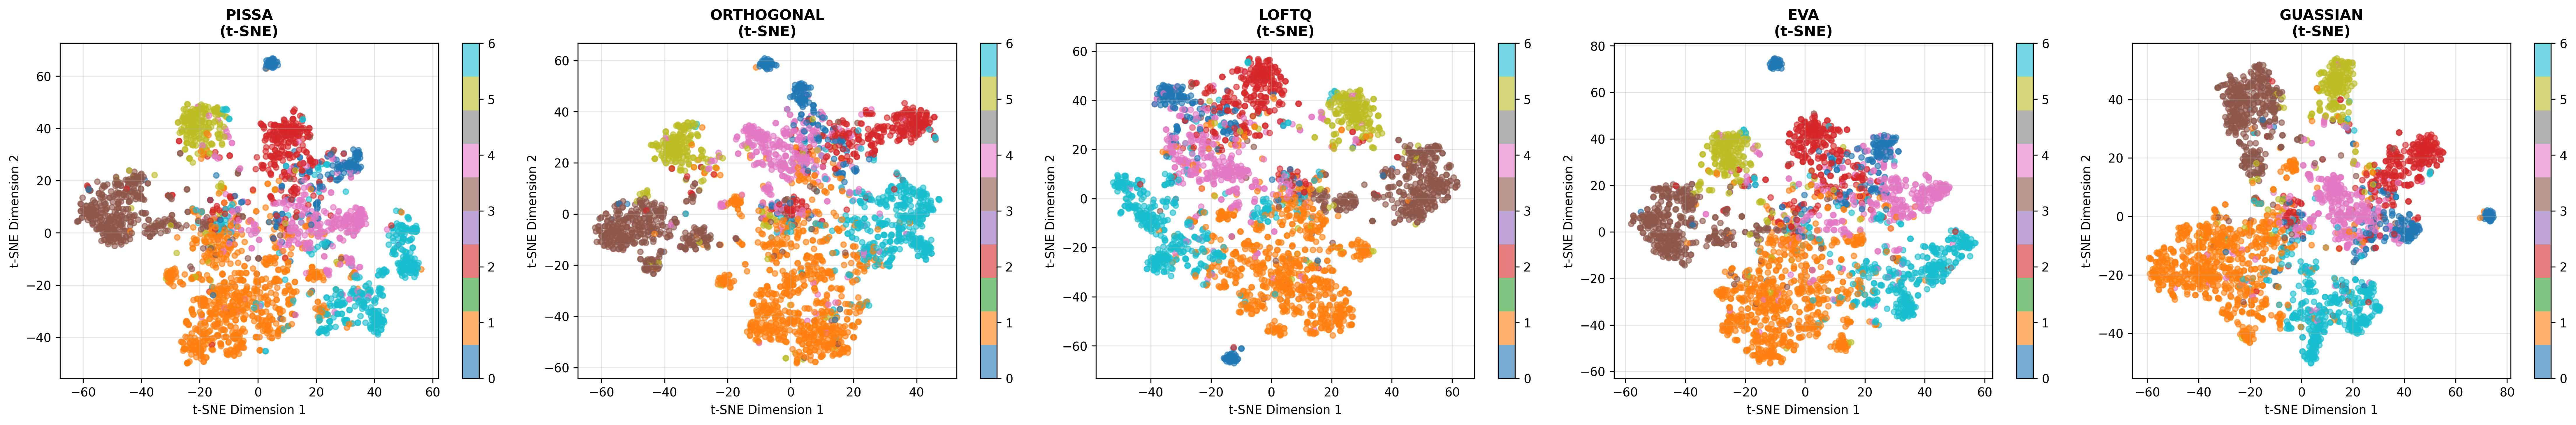
\includegraphics[width=\textwidth]{images/llama_3.2_1B_cora_lora_tsne_comparison.png}
	\caption{Overview of textual embeddings obtained from LLMs using different initial parameters.}
	\small
	Two-dimensional visualization of node embeddings using the t-SNE method for different versions of the language model trained on the Cora dataset. Differences in clustering patterns indicate the effect of parameter initialization on the semantic representations of nodes.
	\label{fig:tsne}
\end{figure}

As described in the proposed method, an LLM is fine-tuned on node text data specifically for the graph text classification task. Upon completion of the training process, node-level representations are extracted by applying a mean pooling operator over the textual representations associated with each node.

To qualitatively compare these representations, the node embeddings generated by each model version were mapped into a two-dimensional space using the t-SNE method  \citep{cai2022tsne}, the results of which are shown in Figure \ref{fig:tsne}. As evident from the plots, each trained language model, despite using identical data and labels, has achieved distinct spatial patterns and node clusterings. These variations demonstrate that changes in the initialization of trainable parameters can lead to distinct semantic interpretations of node texts, consequently producing diverse node-level representations.

\subsection{Why do different LoRA initializations yield different representations?}\label{sec:initDiversity}

\revcommon[R1,R2,R4]{The t-SNE plots in Figure~\ref{fig:tsne} show that the five views differ, but they cannot tell whether the difference is caused by the initialization or by the randomness of training. We therefore follow the effect of the initialization through each stage of the pipeline: the adapter weights, the LLM embeddings, the GNN embeddings and the GNN predictions. We report the analysis for CiteSeer with Gemma-2-2B.}

\paragraph{\revcommon{Mechanism.}}
\revcommon[R1,R2,R4]{LoRA adds a rank-$r$ update $\mathbf{B}\mathbf{A}$ to a frozen weight $\mathbf{W}\in\mathbb{R}^{d_{out}\times d_{in}}$, so the adapter reads its input through the $r$-dimensional row space of $\mathbf{A}$ and writes into the column space of $\mathbf{B}$. When $\mathbf{B}$ starts at zero (Gaussian, Orthogonal and EVA), the first gradient of $\mathbf{B}$ is $\nabla_{\mathbf{B}}\mathcal{L}=\mathbf{g}\,(\mathbf{A}\mathbf{x})^{\top}$, so learning is confined to the input directions selected by the initial $\mathbf{A}$, and $\mathbf{A}$ itself moves little during fine-tuning \citep{zhu2024asymmetry}. Each strategy chooses these directions differently: PiSSA takes the top-$r$ singular vectors of $\mathbf{W}$ \citep{meng2024pissa}, LoftQ the singular vectors of the quantization residual \citep{li2023loftq}, EVA the principal directions of the input activations \citep{paischer2024eva}, and Gaussian/Orthogonal random directions \citep{Hu2021LoRA, zhang2025orthogonal}. Because $r\ll d$ ($8$ vs.\ $2304$ for Gemma-2-2B), two such subspaces overlap very little, so the initialization decides which part of the pretrained representation each adapter is able to modify.}

\paragraph{\revcommon{Experimental design.}}
\revcommon[R1,R2,R4]{To separate the initialization from training randomness, each of the five initializations was fine-tuned with four LoRA seeds, giving a pool of $5\times4=20$ members.
The LoRA seed controls the 60/20/20 split used for fine-tuning, the classification-head initialization, the data order, the dropout masks and, for random initializations, the random matrix $\mathbf{A}$. A GraphSAGE model was trained on every member with the same GNN seed, so two members differ only in their LoRA initialization and/or LoRA seed. For each pair of members we measure a distance and group the pairs into \emph{seed-only} pairs (same initialization, different seed; 30 pairs), \emph{init-only} pairs (different initialization, same seed; 40 pairs) and pairs that differ in \emph{both} (120 pairs). Adapter distances are one minus the mean subspace overlap $\|\mathbf{Q}_i^{\top}\mathbf{Q}_j\|_F^2/r$ over the 104 LoRA layers, where $\mathbf{Q}$ is an orthonormal basis of the row space of $\mathbf{A}$ or the column space of $\mathbf{B}$; embedding distances are $1-$ linear CKA \citep{kornblith2019cka}; prediction distance is the label disagreement on the test nodes. On these pair groups we ask two different questions at every stage of the pipeline:}
\begin{itemize}
    \item \revcommon[R1,R2,R4]{\textbf{Q1} (does the initialization add diversity beyond training randomness?): are pairs that differ in both initialization and seed farther apart than pairs that differ in the seed only? Both groups differ in the seed, so a larger distance in the first group is caused by the initialization. The $p$-value comes from 2000 permutations of the initialization labels within each seed.}
    \item \revcommon[R1,R2,R4]{\textbf{Q2} (is the initialization a \emph{larger} source of diversity than training randomness?): is the init-only distance larger than the seed-only distance, i.e.\ is the ratio init-only/seed-only above one? This is the comparison with an ensemble of one initialization trained with different seeds.}
\end{itemize}
\revcommon[R1,R2,R4]{Q1 can hold while Q2 does not: the initialization can add diversity on top of the seed without adding more than a new seed would. Section~\ref{sec:initQ1} answers Q1 and Section~\ref{sec:initQ2} answers Q2.}

% ---------------------------------------------------------------------------
\subsubsection{\revcommon{Q1: Does the initialization add diversity beyond training randomness?}}\label{sec:initQ1}

\begin{table*}[t]
\centering\color{revshared}
\caption{Q1. Pool distances between members that differ in seed only, initialization only, or both (CiteSeer, Gemma-2-2B; larger is more diverse). $p$: permutation test of \emph{both} vs.\ \emph{seed-only}.}
\label{tab:seed_vs_init}
\small
\begin{tabular*}{\textwidth}{@{\extracolsep{\fill}} llcccc @{}}
\toprule
\textbf{Stage} & \textbf{Distance} & \textbf{Seed-only} & \textbf{Init-only} & \textbf{Both} & \textbf{$p$ (Q1)} \\
\midrule
Adapter weights & $1-$ overlap, row($\mathbf{A}$) & 0.641 & 0.995 & 0.995 & $<0.001$ \\
                & $1-$ overlap, col($\mathbf{B}$) & 0.613 & 0.976 & 0.980 & $<0.001$ \\
                & $1-\cos$, update $\mathbf{B}\mathbf{A}$ & 0.638 & 0.999 & 0.999 & $<0.001$ \\
\midrule
LLM embeddings  & $1-$ CKA & 0.265 & 0.288 & 0.320 & $<0.001$ \\
GNN embeddings  & $1-$ CKA & 0.074 & 0.080 & 0.093 & $<0.001$ \\
GNN predictions & disagreement & 0.088 & 0.087 & 0.098 & $<0.001$ \\
\bottomrule
\end{tabular*}
\end{table*}

\paragraph{\revcommon{Adapter weights.}}
\revcommon[R1,R2,R4]{Table~\ref{tab:seed_vs_init} shows that, in weight space, adapters trained from different initializations end in almost orthogonal subspaces (distance $0.98$--$1.00$), and that changing the initialization adds distance on top of changing the seed ($p<0.001$). Table~\ref{tab:spectral} locates the trained adapters in the spectrum of the pretrained weights. PiSSA adapters remain in the top-$r$ singular subspace after training (overlap $0.98$ for col($\mathbf{B}$), about $170\times$ the random level), LoftQ adapters lean toward the dominant output directions ($16\times$ random), and Gaussian, Orthogonal and EVA adapters lie close to the random level. These positions vary by at most $0.002$ across seeds. Each initialization therefore keeps a stable and distinct region of the weight spectrum in which it adapts the model.}

\begin{table}[htbp]
\centering\color{revshared}
\caption{Overlap of the trained adapters with the top-$r$ and bottom-$r$ singular subspaces of the pretrained weights (CiteSeer, Gemma-2-2B). Random subspaces give $0.0058$ for col($\mathbf{B}$) and $0.0036$ for row($\mathbf{A}$).}
\label{tab:spectral}
\small
\begin{tabular}{lcccc}
\toprule
\textbf{Initialization} & \textbf{col($\mathbf{B}$) top} & \textbf{col($\mathbf{B}$) bottom} & \textbf{row($\mathbf{A}$) top} & \textbf{row($\mathbf{A}$) bottom} \\
\midrule
PiSSA      & 0.976 & 0.000 & 0.959 & 0.000 \\
LoftQ      & 0.093 & 0.004 & 0.005 & 0.004 \\
Orthogonal & 0.008 & 0.008 & 0.006 & 0.004 \\
Gaussian   & 0.010 & 0.010 & 0.004 & 0.004 \\
EVA        & 0.009 & 0.011 & 0.004 & 0.004 \\
\bottomrule
\end{tabular}
\end{table}

\paragraph{\revcommon{From weights to representations and predictions.}}
\revcommon[R1,R2,R4]{Mantel tests \citep{mantel1967} between the pool distance matrices of consecutive stages (Table~\ref{tab:mantel}) show that the weight-space differences propagate through the whole pipeline: members whose adapter updates differ more also have more different LLM embeddings ($\rho=0.57$, $p<0.001$), the LLM-embedding distance is related to the GNN-embedding distance ($\rho=0.59$) and to the prediction disagreement ($\rho=0.53$), and the GNN-embedding distance predicts the prediction disagreement ($\rho=0.77$; all $p<0.001$). Along this chain the diversity is compressed: nearly orthogonal adapters produce embeddings with CKA of about $0.7$, and the GNNs, which propagate over the same graph, disagree on about $9\%$--$10\%$ of the test nodes.} \revcommon[R1,R2,R4]{At every stage, members that differ in both initialization and seed are the most diverse, and the initialization adds significant diversity on top of the seed ($p<0.001$, Table~\ref{tab:seed_vs_init}). The answer to Q1 is therefore positive at all four stages.}

\begin{table}[htbp]
\centering\color{revshared}
\caption{Mantel correlation (Spearman $\rho$, 2000 permutations) between the pool distance matrices of successive stages (CiteSeer, Gemma-2-2B).}
\label{tab:mantel}
\small
\begin{tabular}{llcc}
\toprule
\textbf{From} & \textbf{To} & \textbf{$\rho$} & \textbf{$p$} \\
\midrule
Adapter update ($\mathbf{B}\mathbf{A}$) & LLM embeddings  & 0.57 & $<0.001$ \\
Adapter col($\mathbf{B}$)               & LLM embeddings  & 0.16 & 0.022 \\
LLM embeddings                          & GNN embeddings  & 0.59 & $<0.001$ \\
LLM embeddings                          & GNN predictions & 0.53 & $<0.001$ \\
GNN embeddings                          & GNN predictions & 0.77 & $<0.001$ \\
Adapter col($\mathbf{B}$)               & GNN predictions & 0.28 & 0.001 \\
\bottomrule
\end{tabular}
\end{table}

\paragraph{\revcommon{Systematic differences between initializations.}}
\revcommon[R1,R2,R4]{If the initializations produced only random variation, their differences would not repeat across seeds. We tested this with a two-way ANOVA of the per-class test accuracy with initialization and class as factors and the four seeds as replicates, so the residual is exactly the seed variation. The initialization has a significant effect ($F(4,90)=4.23$, $p=0.003$, partial $\eta^2=0.16$): the differences in quality between initializations are larger than the differences between seeds. They are most visible on the hardest class, where PiSSA reaches $40.0\%$ and Orthogonal $25.0\%$ averaged over seeds. Of the $111$ test nodes that some initialization misclassifies in every seed, $63$ are not persistent errors of every initialization, i.e.\ they can be recovered by another view. Combining four initializations gives more test nodes a correct $k$-NN majority than combining four seeds of one initialization ($83.7\%$ vs.\ $82.4\%$ for the LLM embeddings, $85.2\%$ vs.\ $84.7\%$ for the GNN embeddings; $72.1\%$ and $76.9\%$ for a single view).}

\paragraph{\revcommon{Complementarity.}}
\revcommon[R1,R2,R4]{Diversity is useful only if the members make different errors rather than more errors. We therefore relate the diversity of the members to the gain of their ensemble. To isolate the effect of diversity from the trainable ensemble head, all ensembles in this analysis are uniform averages of the class probabilities, so no weights are fitted. For a uniform average the ambiguity decomposition \citep{krogh1995ensemble} is exact: the ensemble error equals the average member error minus the ambiguity (the spread of the members around the ensemble), so larger diversity at equal member quality directly lowers the ensemble error. Over all $k$-member subsets of the pool, the mean pairwise disagreement is positively correlated with the ensemble gain over the mean member (Spearman $\rho=0.26$, $0.24$, $0.16$ and $0.11$ for $k=2,3,4,5$; all $p<10^{-3}$), and at every ensemble size the gain increases monotonically with the number of distinct initializations in the ensemble (Figure~\ref{fig:div_gain}; for $k=4$ from $+0.74$ pp with one initialization to $+0.98$ pp with four). The pairwise complementarity measures of \citet{kuncheva2003diversity} lead to the same picture: an oracle that picks the correct member is $2.5$--$2.8$ pp more accurate than the better member of a pair, and the oracle gain is largest for pairs that differ in both initialization and seed.}

\begin{figure}[htbp]
	\centering\color{revshared}
	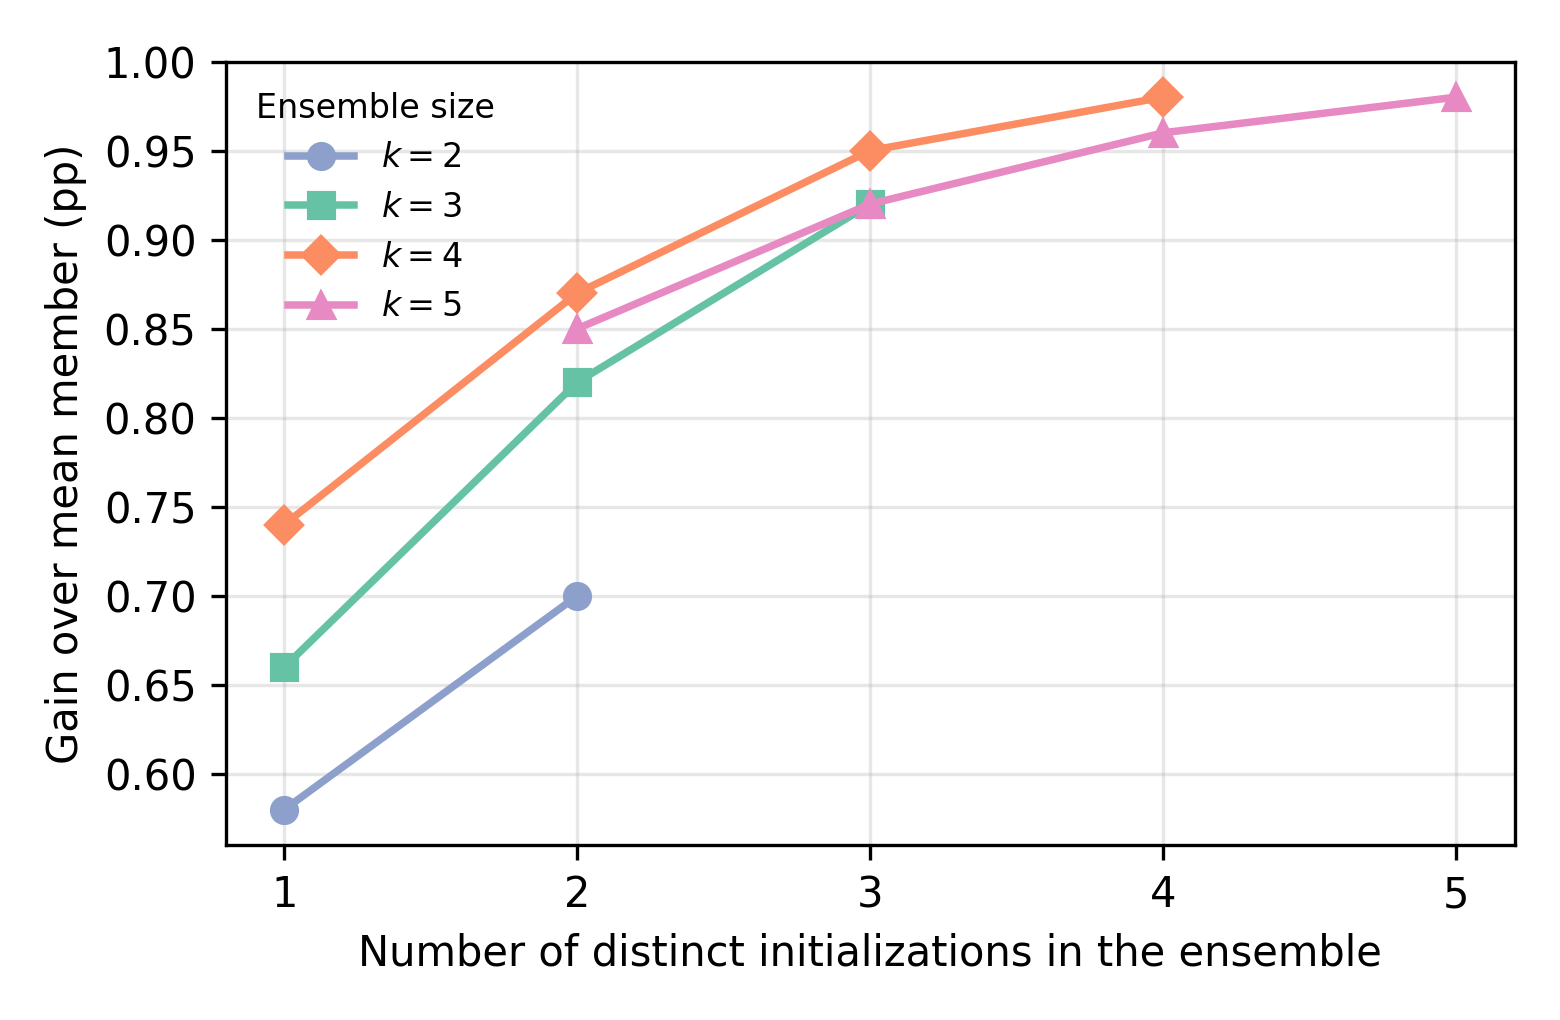
\includegraphics[width=0.7\textwidth]{images/gemma2_2B_citeseer_gain_vs_distinct_inits.png}
	\caption{Ensemble gain over the mean member as a function of the number of distinct initializations among the $k$ members, averaged over all $k$-member subsets of the CiteSeer pool (Gemma-2-2B, uniform averaging).}
	\label{fig:div_gain}
\end{figure}

% ---------------------------------------------------------------------------
\subsubsection{\revcommon{Q2: Is the initialization a larger source of diversity than training randomness?}}\label{sec:initQ2}

\revcommon[R1,R2,R4]{Q2 compares two members of different initializations with two members of the same initialization trained with different seeds, which is the seed-ensemble baseline requested by the reviewers. Table~\ref{tab:q2} (left) reports the ratio of init-only to seed-only distance in the pool above. In weight space the initialization clearly dominates: init-only distances are about $1.6$ times the seed-only distances (one-sided Mann--Whitney $p\leq0.006$), and for the deterministic initializations the seed barely moves the adapter (seed-only distance of the update: PiSSA $0.06$, LoftQ $0.14$). Downstream the two effects become similar in size: the ratio is $1.09$ for the LLM embeddings ($p=0.06$), $1.08$ for the GNN embeddings ($p=0.16$) and $0.99$ for the predictions ($p=0.50$). The local neighbourhoods are the exception: the $10$ nearest neighbours of a node change more between initializations than between seeds in both the LLM embeddings (ratio $1.11$, $p=0.005$) and the GNN embeddings ($1.08$, $p=0.010$). PERMANOVA attributes more of the variance to the initialization than to the seed at every stage ($R^2$ $0.35$, $0.41$ and $0.31$ for the initialization vs.\ $0.24$, $0.29$ and $0.28$ for the seed in the LLM embeddings, GNN embeddings and predictions).}

\revcommon[R1,R2,R4]{In this pool, however, the seed-only baseline mixes three sources of variation: a LoRA seed also selects the fine-tuning split and, for Gaussian, Orthogonal and EVA, draws a new random initialization, while the data order and the dropout masks were the same for all seeds. Two ``seeds'' of Gaussian are therefore two random initializations fine-tuned on different labelled nodes, which is why their adapters are as far apart as two different initializations (seed-only distance $0.97$--$1.00$). We therefore designed a controlled experiment in which the seed-only baseline contains nothing but training randomness.}

\paragraph{\revcommon{Controlled experiment.}}
\revcommon[R1,R2,R4]{We built four controlled pools: Cora and CiteSeer, each with Gemma-2-2B (the LLM of the pool above, 104 LoRA layers) and with LLaMA-3.2-1B (64 LoRA layers). In each pool the five initializations are fine-tuned with four training seeds (42--45) under three constraints: (i) every member is fine-tuned on the same split, which is also the split of its GNN, so no member has seen the labels of the test nodes; (ii) the random draw of the LoRA initialization is fixed by a separate initialization seed, so all members of one strategy start from the identical adapter; (iii) the training seed sets the classification-head initialization, the data order and the dropout masks. A seed-only pair is then exactly the same initialization trained with a different random seed, and an init-only pair differs only in the initialization strategy. As before, a GraphSAGE model with a fixed GNN seed is trained on every member. At each of the four stages we use one distance fixed in advance ($1-\cos$ of the adapter updates, $1-$CKA of the LLM and of the GNN embeddings, prediction disagreement), and the $10$-NN neighbourhood distance as a secondary measure. Because pairs that share a member are not independent, the ratio init-only/seed-only is tested with a crossed bootstrap that resamples initializations and seeds with replacement; the initialization is called a larger source of diversity at a stage if the one-sided bootstrap $p$ for ratio $\leq1$ is below $0.05$. Across pools we report how many ratios are above one and their geometric mean.}
% Pools: results/diversity_q2/*_q2ctl_split42_init0_SAGE_report.txt; across pools: q2_across_pools.txt.
% CiteSeer/LLaMA has two collapsed Orthogonal members (seeds 43/44, 22%/18% GNN acc), kept in the pool.
% CiteSeer/Gemma has 19 members: the EVA-42 embedding cache failed.

\begin{table*}[t]
\centering\color{revshared}
\caption{Q2. Ratio of init-only to seed-only distance ($>1$: the initialization changes members more than the seed). Left: pool of Table~\ref{tab:seed_vs_init}; right: controlled pools (bootstrap $p$). Bold: $p<0.05$; $^\ddagger$two members collapsed.}
\label{tab:q2}
\footnotesize
\setlength{\tabcolsep}{3pt}
\begin{tabular*}{\textwidth}{@{\extracolsep{\fill}} lcc|cc|cc|c @{}}
\toprule
 & \multicolumn{2}{c|}{\textbf{Original pool}} & \multicolumn{2}{c|}{\textbf{Controlled: Gemma-2-2B}} & \multicolumn{2}{c|}{\textbf{Controlled: LLaMA-3.2-1B}} & \\
\textbf{Stage} & \textbf{Ratio} & \textbf{$p$} & \textbf{Cora} & \textbf{CiteSeer} & \textbf{Cora} & \textbf{CiteSeer}$^\ddagger$ & \textbf{Geo.\ mean} \\
\midrule
Adapter update ($\mathbf{B}\mathbf{A}$) & 1.56 & \textbf{0.006} & \textbf{1.73 ($<$0.001)} & \textbf{1.84 ($<$0.001)} & \textbf{1.83 ($<$0.001)} & \textbf{1.79 ($<$0.001)} & 1.80 \\
LLM embeddings (CKA)   & 1.09 & 0.062 & 1.25 (0.127) & 1.19 (0.147) & 1.30 (0.060) & 1.25 (0.211) & 1.25 \\
GNN embeddings (CKA)   & 1.08 & 0.155 & 1.23 (0.159) & 1.25 (0.095) & 1.20 (0.172) & 1.44 (0.299) & 1.27 \\
GNN predictions        & 0.99 & 0.500 & 1.12 (0.208) & \textbf{1.21 (0.048)} & 1.13 (0.132) & 1.25 (0.344) & 1.18 \\
\midrule
LLM embeddings ($k$-NN) & 1.11 & \textbf{0.005} & \textbf{1.13 (0.022)} & \textbf{1.14 (0.007)} & \textbf{1.10 (0.038)} & 1.12 (0.122) & 1.12 \\
GNN embeddings ($k$-NN) & 1.08 & \textbf{0.010} & \textbf{1.07 (0.045)} & \textbf{1.10 (0.004)} & 1.04 (0.104) & 1.05 (0.204) & 1.06 \\
\bottomrule
\end{tabular*}
\end{table*}

\revcommon[R1,R2,R4]{Once the seed is the only source of training randomness, the init-only distance is larger than the seed-only distance at every stage, in all four pools and for both LLMs: all $24$ ratios are above one ($1.04$--$1.84$, Table~\ref{tab:q2}, right), whereas in the original pool the ratio was close to one downstream of the adapters. The geometric mean over the pools is $1.80$ for the adapter updates, $1.25$ and $1.27$ for the LLM and GNN embeddings, $1.18$ for the predictions, and $1.12$ and $1.06$ for the two neighbourhood measures. The seed-only distances drop accordingly: in weight space they fall to $0.54$--$0.58$ (from $0.64$), because a deterministic initialization trained with another seed ends in almost the same adapter, while two initializations stay nearly orthogonal ($0.997$--$0.999$). The initialization is a significantly larger source of diversity in weight space in every pool (ratios $1.73$--$1.84$, all $p<0.001$, lower confidence bound $\geq1.10$), and in the local neighbourhoods of the LLM embeddings in three of the four pools (ratios $1.10$--$1.14$, $p\leq0.038$) and of the GNN embeddings in both Gemma pools ($1.07$, $p=0.045$; $1.10$, $p=0.004$). For the predictions the ratio is significant on CiteSeer with Gemma ($1.21$, $p=0.048$) and has the same direction in the other three pools ($1.12$--$1.25$). For the global embedding geometry measured by CKA the ratio is $1.19$--$1.44$ in all pools, but with five initializations and four seeds the crossed bootstrap cannot exclude a ratio of one ($p=0.06$--$0.30$). PERMANOVA agrees with this picture: in every pool and at every primary stage the initialization explains $35$--$61\%$ of the variance of the distances ($p\leq0.018$), and the training seed only $5$--$20\%$ ($p\geq0.17$). The LLaMA pools give the same ratios as the Gemma pools, so the result does not depend on the LLM. Their $p$-values are larger on CiteSeer because two Orthogonal members collapsed during fine-tuning; these outliers inflate the spread of the seed-only distances and widen the confidence intervals (e.g.\ $[0.37, 14.3]$ for the GNN embeddings). The CiteSeer/Gemma pool has $19$ members because the embeddings of one member (EVA, seed 42) could not be extracted.}

\paragraph{\revcommon{Ensembles of one initialization with several seeds.}}
\revcommon[R1,R2,R4]{Table~\ref{tab:seed_multi_ensemble} compares ensembles of equal size built from one initialization with four seeds and from four initializations with one seed. At the same average member error, the multi-init ensembles are slightly more accurate ($82.85\%$ vs.\ $82.76\%$) and lose less to their best member ($-0.61$ vs.\ $-1.00$ pp). No uniform average exceeds its strongest member: with 60\% of the nodes labelled the members are already strong, and equal weights let the weaker members pull the average down. Recovering this loss requires member- and class-specific weights, which is what the trainable ensemble heads of DIVERGE provide (Sections~\ref{sec:ensemble_weight_analysis} and~\ref{sec:trainable_vs_avg}).}

\begin{table}[htbp]
\centering\color{revshared}
\caption{Uniform-average ensembles of $k=4$ members: one initialization with four seeds (seed-only, 5 ensembles) or four initializations with one seed (multi-init, 20 ensembles). CiteSeer, Gemma-2-2B; gains in pp.}
\label{tab:seed_multi_ensemble}
\small
\begin{tabular}{lccccc}
\toprule
\textbf{Family} & \textbf{Ens.\ acc.} & \textbf{Gain vs.\ mean} & \textbf{Gain vs.\ best} & \textbf{Avg.\ member error} & \textbf{Ambiguity} \\
\midrule
Seed-only  & 82.76 & +0.74 & $-1.00$ & 0.2732 & 0.0128 \\
Multi-init & 82.85 & +0.84 & $-0.61$ & 0.2732 & 0.0124 \\
\bottomrule
\end{tabular}
\end{table}

\revcommon[R1,R2,R4]{In summary, the initialization determines where in the pretrained weight spectrum each adapter operates, and this choice is stable across seeds. The differences it creates in weight space propagate to the node embeddings, the local neighbourhoods and the predictions, and at every stage the initialization adds significant diversity on top of training randomness (Q1). When training randomness is isolated, the initialization is also a larger source of diversity than the seed (Q2): the ratio is above one at every stage in all four pools (two datasets, two LLMs), significantly so in weight space in every pool and in the local neighbourhoods in most pools, and in the predictions on CiteSeer with Gemma; for the global embedding geometry the effect has the same direction but is not significant with pools of this size.}

\subsection{\revcommon{Behaviour of the Adaptive Ensemble Weights}}
\label{sec:ensemble_weight_analysis}

\revcommon[R1,R2,R4]{The trainable ensemble heads add parameters on top of the GNN pool, so it is necessary to show what these parameters buy and when learned weights are preferable to simple averaging. We analyse this on Cora with three LLM encoders (LLaMA-3.2-1B, SmolLM2-1.7B, Gemma-2-2B) and on CiteSeer with LLaMA-3.2-1B, using GraphSAGE and the supervised split. For each setting we build one pool from a single LoRA seed per initialization and retrain the five view GNNs with four GNN seeds; each fusion head is additionally refitted with three fusion seeds (12 runs). Because this pool uses one LoRA seed and retrained GNNs, the absolute accuracies differ slightly from Table~\ref{tab:diverge_llm_encoders}. All fusion rules are applied to exactly the same view GNNs, nodes and labels, so every difference between rules is caused by the fusion step alone.}

\revcommon[R1,R2,R4]{To avoid any optimistic bias, each learned head is fitted on the GNN logits of one half of the validation nodes, its training epoch and hyperparameters are selected on the other half, and the test nodes are used only once for the final evaluation. We do not fit the heads on training-node logits, because the GNNs were trained on those nodes and their logits are over-confident. Significance is tested with paired tests over runs; since the runs that share a GNN seed are not independent, we also test the four GNN-seed means, which is the conservative test.}

\paragraph{\revcommon{Where can a fusion rule change the prediction?}}
\revcommon[R1,R2,R4]{All heads of DIVERGE combine the view logits with non-negative weights that sum to one (softmax-normalised). Such a convex combination cannot change the prediction of a node on which all views predict the same label. Table~\ref{tab:ens_agreement} reports the share of such unanimous test nodes together with uniform averaging and an oracle that counts a node as correct if at least one view is correct. No learned head is involved in this table.}

\begin{table}[ht]
\centering
\caption{\revcommon[R1,R2,R4]{Share of unanimous test nodes, test accuracy (\%) of uniform logit averaging, and of an oracle correct if any view is correct (mean over 12 runs). $^\dagger$The Orthogonal view collapsed (23.4\% alone).}}
\label{tab:ens_agreement}
\begin{tabular}{l c c c c}
\hline
Setting & Unanimous nodes & Uniform average & Oracle & Headroom (pp) \\
\hline
Cora, LLaMA-3.2-1B        & 87.9\% & 90.13 & 93.54 & +3.4 \\
Cora, SmolLM2-1.7B        & 89.4\% & 90.08 & 93.59 & +3.5 \\
Cora, Gemma-2-2B          & 88.4\% & 91.05 & 94.51 & +3.5 \\
CiteSeer, SmolLM2-1.7B    & 84.1\% & 79.51 & 85.07 & +5.6 \\
CiteSeer, LLaMA-3.2-1B$^\dagger$ & 21.4\% & 79.19 & 88.24 & +9.0 \\
\hline
\end{tabular}
\end{table}

\revcommon[R1,R2,R4]{Two conclusions follow. First, the views are complementary: in every setting the oracle is 3.4--9.0 percentage points above uniform averaging, so the pool contains correct predictions that averaging does not use. Second, when the views are of similar quality, 84\%--89\% of the test nodes are unanimous, so any fusion rule can act only on the remaining 11\%--16\%. This bounds the possible gain of a learned head over averaging on balanced pools.}

\paragraph{\revcommon{Why uniform averaging is already strong on balanced views.}}
\revcommon[R1,R2,R4]{Averaging raw logits gives each view an equal vote only if the views produce logits of similar scale. For LLaMA-3.2-1B and Gemma-2-2B on Cora, the effective share of each view in the uniform logit sum lies between 0.180 and 0.211 (an equal vote is 0.200). The views also contribute almost equally to the ensemble: the exact Shapley value of each view, computed over all 31 view subsets of the uniform average, lies between 10.8 and 12.6 percentage points of test accuracy for all three Cora encoders. When the views are balanced in this way, equal weights are already close to optimal. The CiteSeer pool with LLaMA-3.2-1B is different: its Orthogonal view collapsed during fine-tuning (23.4\% accuracy alone; the same instability is visible in the large standard deviation of this view in Table~\ref{tab:diverge_llm_encoders}). Its share of the uniform logit sum drops to 0.145, but its Shapley value is negative ($-4.1$ pp): uniform averaging is worse \emph{with} this view than without it, and it has no mechanism to detect this.}

\paragraph{\revcommon{What do the extra parameters buy?}}
\revcommon[R1,R2,R4]{Table~\ref{tab:ens_fusion_rules} compares the learned heads with parameter-free rules and with stacking, a standard learned combiner (multinomial logistic regression on the concatenated view logits) that has more parameters but no convexity constraint. The view-level head learns one weight per view ($M=5$ parameters) and the class-level head one weight per view and class ($M\times C$ parameters); both are softmax-normalised. All heads are trained and selected as described above.}

\begin{table}[ht]
\centering
\caption{\revcommon[R1,R2,R4]{Test accuracy (\%) of fusion rules on the same five view GNNs (mean $\pm$ std, 12 runs); learned heads are fitted and selected on disjoint validation halves. Bold: best per column; $^\dagger$see Table~\ref{tab:ens_agreement}.}}
\label{tab:ens_fusion_rules}
\small
\setlength{\tabcolsep}{3pt}
\resizebox{\textwidth}{!}{%
\begin{tabular}{l r c c c c c}
\hline
 & & \multicolumn{3}{c}{Cora} & \multicolumn{2}{c}{CiteSeer} \\
Rule & \#Params & LLaMA-3.2-1B & SmolLM2-1.7B & Gemma-2-2B & LLaMA-3.2-1B$^\dagger$ & SmolLM2-1.7B \\
\hline
Best single view (by validation) & -- & 90.22{\scriptsize$\pm$1.12} & \textbf{90.45}{\scriptsize$\pm$1.68} & 90.45{\scriptsize$\pm$1.45} & 80.33{\scriptsize$\pm$1.08} & 80.29{\scriptsize$\pm$1.34} \\
Uniform average of logits & 0 & 90.13{\scriptsize$\pm$0.83} & 90.08{\scriptsize$\pm$1.18} & \textbf{91.05}{\scriptsize$\pm$0.74} & 79.19{\scriptsize$\pm$1.70} & 79.51{\scriptsize$\pm$0.43} \\
Uniform average of probabilities & 0 & 90.31{\scriptsize$\pm$0.70} & 90.13{\scriptsize$\pm$1.18} & 91.01{\scriptsize$\pm$0.73} & 80.05{\scriptsize$\pm$0.91} & 79.86{\scriptsize$\pm$0.64} \\
Majority vote & 0 & 90.45{\scriptsize$\pm$0.72} & 89.81{\scriptsize$\pm$1.18} & 90.54{\scriptsize$\pm$0.79} & 80.17{\scriptsize$\pm$0.50} & 79.66{\scriptsize$\pm$0.34} \\
Entropy-weighted average & 0 & 90.41{\scriptsize$\pm$0.80} & 90.13{\scriptsize$\pm$1.14} & 90.96{\scriptsize$\pm$0.76} & 80.45{\scriptsize$\pm$1.11} & 79.58{\scriptsize$\pm$0.41} \\
\hline
Stacking (logistic regression) & 252 / 186 & 89.70{\scriptsize$\pm$1.26} & 89.04{\scriptsize$\pm$1.65} & 89.82{\scriptsize$\pm$1.45} & 79.38{\scriptsize$\pm$1.06} & 78.19{\scriptsize$\pm$1.05} \\
DIVERGE view-level weights & 5 / 5 & 90.53{\scriptsize$\pm$0.68} & 90.21{\scriptsize$\pm$1.27} & \textbf{91.05}{\scriptsize$\pm$0.77} & 80.45{\scriptsize$\pm$0.90} & 80.34{\scriptsize$\pm$0.88} \\
DIVERGE class-level weights & 35 / 30 & 90.64{\scriptsize$\pm$0.87} & 90.24{\scriptsize$\pm$1.27} & 90.97{\scriptsize$\pm$0.70} & \textbf{80.79}{\scriptsize$\pm$0.79} & 80.00{\scriptsize$\pm$0.73} \\
DIVERGE node-conditioned (Method~1) & 3.5k--7.8k & \textbf{90.67}{\scriptsize$\pm$0.82} & 90.16{\scriptsize$\pm$1.47} & 90.67{\scriptsize$\pm$0.93} & 80.22{\scriptsize$\pm$0.86} & \textbf{80.55}{\scriptsize$\pm$0.72} \\
\hline
\end{tabular}}
\end{table}

\revcommon[R1,R2,R4]{Three results follow from Table~\ref{tab:ens_fusion_rules}.}

\revcommon[R1,R2,R4]{\textit{(i) The constraint makes the extra parameters safe.} An unconstrained combiner fitted on the same validation nodes overfits: stacking is below uniform averaging on all three Cora encoders ($-0.43$ to $-1.23$ pp). The softmax-constrained class-level head of DIVERGE is more accurate than stacking in every setting ($+0.94$ to $+1.41$ pp) and in all 16 GNN-seed means (Wilcoxon signed-rank $p<0.001$); the view-level head is better in 15 of 16 ($p<0.001$). Restricting the learned weights to a convex combination is therefore what allows them to be fitted on a few hundred labelled nodes without overfitting.}

\revcommon[R1,R2,R4]{\textit{(ii) On balanced views, the learned weights match uniform averaging.} On the three Cora pools the view- and class-level heads are within $-0.08$ to $+0.51$ pp of uniform averaging and lose to it in at most 3 of 12 runs; the differences are not significant at the GNN-seed level ($p\geq0.12$). This agrees with the analysis above: when 88\%--89\% of the nodes are unanimous and the views contribute equally, the optimal weights are close to uniform, and the extra parameters neither help nor hurt. The node-conditioned head, which has thousands of parameters, brings no further gain over the class-level head on these datasets.}

\revcommon[R1,R2,R4]{\textit{(iii) When one view is weak, the learned weights improve over averaging.} On the CiteSeer pool with the collapsed Orthogonal view, the class-level head improves uniform averaging by $+1.59$ pp (80.79 vs.\ 79.19), is better in 10 of 12 runs (paired $t$-test $p=0.002$), and is also above the best single view (80.33). It is significantly more accurate than both stacking ($+1.41$ pp) and the node-conditioned head ($+0.56$ pp; GNN-seed level $p=0.005$ and $p=0.014$). Uniform averaging, in contrast, is pulled below the best single view by the collapsed member. The vulnerability of averaging grows with the influence of such a view: when the logits of the weakest CiteSeer view are duplicated $k=1,\dots,4$ times, which raises its share of the uniform vote from $0.20$ to $0.56$, the accuracy of uniform averaging drops from 79.19\% to 62.77\%.}

\revcommon[R1,R2,R4]{In summary, the learned weights of DIVERGE improve over simple averaging when the views are unbalanced, as when one LoRA initialization fails on a dataset, and perform on par with it when the views are balanced. Because this failure cannot be known in advance for a new dataset, the low-cost view- and class-level heads (5--35 parameters) act as a safeguard that removes the influence of a weak view at no cost in accuracy on balanced pools.}



\subsection{Performance Comparison of Trainable Ensemble Learning vs. Simple Averaging}\label{sec:trainable_vs_avg}

In Table \ref{tab:diverge_llm_encoders}, the performance of the three proposed trainable ensemble learning methods is compared with the simple averaging-based ensemble approach (Uniform) across the aforementioned datasets in terms of accuracy. Based on the obtained results, all three proposed trainable methods deliver superior performance compared to the simple averaging approach.

The differences among the three trainable methods are small: they lie within 0.9 points of each other in all 21 encoder--dataset pairs. Method 2 is the most accurate (or tied) in 12 of the 21 pairs and Method 3 in 8, so no single method dominates.

\subsection{DIVERGE with Different LLM Encoders}\label{sec:llm_encoders}

\begin{table}[htbp]
\centering
\caption{Accuracy of DIVERGE with different LLM encoders. For each encoder, the first five rows report the GNN trained on the text embeddings obtained with each LoRA initialization approach, followed by the three DIVERGE ensemble methods.}
\label{tab:diverge_llm_encoders}

\small
\setlength{\tabcolsep}{3pt}
\begin{tabular*}{\textwidth}{@{\extracolsep{\fill}} lccccccc @{}}
\toprule
\multirow{2}{*}{\textbf{Method}} & \multicolumn{7}{c}{\textbf{Accuracy (\%)}} \\
\cmidrule(lr){2-8}
 & \textbf{Cora} & \textbf{CiteSeer} & \textbf{PubMed} & \textbf{WikiCS} & \textbf{ArXiv} & \textbf{Computers} & \textbf{Reddit} \\
\midrule
\multicolumn{8}{l}{\textit{LLM encoder: LLaMA-3.2-1B}} \\
\midrule
PiSSA                     & 88.84{\scriptsize$\pm$1.01} & 77.59{\scriptsize$\pm$1.99} & 94.75{\scriptsize$\pm$0.18} & 87.87{\scriptsize$\pm$0.31} & 77.71{\scriptsize$\pm$0.16} & 90.73{\scriptsize$\pm$0.31} & 63.20{\scriptsize$\pm$0.52} \\
Gaussian                  & 88.05{\scriptsize$\pm$1.22} & 77.08{\scriptsize$\pm$0.78} & 93.76{\scriptsize$\pm$0.26} & 87.53{\scriptsize$\pm$0.24} & 76.53{\scriptsize$\pm$0.27} & 89.97{\scriptsize$\pm$0.38} & 58.34{\scriptsize$\pm$0.61} \\
EVA                       & 89.30{\scriptsize$\pm$1.10} & 78.29{\scriptsize$\pm$1.20} & 95.06{\scriptsize$\pm$0.12} & 88.51{\scriptsize$\pm$0.19} & 77.73{\scriptsize$\pm$0.14} & 90.71{\scriptsize$\pm$0.22} & 63.57{\scriptsize$\pm$0.45} \\
LoftQ                     & 88.47{\scriptsize$\pm$1.42} & 77.55{\scriptsize$\pm$1.04} & 94.70{\scriptsize$\pm$0.21} & 88.00{\scriptsize$\pm$0.27} & 77.72{\scriptsize$\pm$0.19} & 90.41{\scriptsize$\pm$0.34} & 61.52{\scriptsize$\pm$0.57} \\
Orthogonal                & 86.86{\scriptsize$\pm$1.34} & 77.11{\scriptsize$\pm$1.05} & 83.67{\scriptsize$\pm$0.42} & 87.61{\scriptsize$\pm$0.33} & 75.50{\scriptsize$\pm$0.43} & 66.62{\scriptsize$\pm$0.68} & 51.07{\scriptsize$\pm$0.72} \\
\cmidrule(lr){1-8}
Uniform (simple average)  & 88.93{\scriptsize$\pm$1.12} & 78.37{\scriptsize$\pm$0.76} & 94.62{\scriptsize$\pm$0.15} & 88.34{\scriptsize$\pm$0.16} & 77.80{\scriptsize$\pm$0.17} & 90.22{\scriptsize$\pm$0.28} & 51.07{\scriptsize$\pm$0.64} \\
DIVERGE Ensemble Method 1 & \textbf{89.80}{\scriptsize$\pm$1.39} & \textbf{79.47}{\scriptsize$\pm$0.97} & \textbf{95.26}{\scriptsize$\pm$0.14} & \textbf{88.47}{\scriptsize$\pm$0.22} & \textbf{78.03}{\scriptsize$\pm$0.21} & \textbf{90.87}{\scriptsize$\pm$0.29} & \textbf{64.80}{\scriptsize$\pm$0.48} \\
DIVERGE Ensemble Method 2 & \textbf{89.90}{\scriptsize$\pm$1.32} & \textbf{79.39}{\scriptsize$\pm$0.85} & \textbf{95.26}{\scriptsize$\pm$0.19} & \textbf{88.72}{\scriptsize$\pm$0.17} & \textbf{78.11}{\scriptsize$\pm$0.18} & \textbf{90.88}{\scriptsize$\pm$0.26} & \textbf{65.59}{\scriptsize$\pm$0.41} \\
DIVERGE Ensemble Method 3 & \textbf{89.94}{\scriptsize$\pm$1.15} & \textbf{79.50}{\scriptsize$\pm$0.81} & \textbf{95.23}{\scriptsize$\pm$0.11} & \textbf{88.59}{\scriptsize$\pm$0.28} & \textbf{78.01}{\scriptsize$\pm$0.24} & \textbf{90.82}{\scriptsize$\pm$0.33} & \textbf{65.68}{\scriptsize$\pm$0.37} \\
\midrule
\multicolumn{8}{l}{\textit{LLM encoder: SmolLM2-1.7B}} \\
\midrule
PiSSA                     & 87.69{\scriptsize$\pm$1.08} & 78.02{\scriptsize$\pm$1.81} & 94.50{\scriptsize$\pm$0.17} & 88.17{\scriptsize$\pm$0.29} & 78.04{\scriptsize$\pm$0.18} & 90.81{\scriptsize$\pm$0.27} & 66.38{\scriptsize$\pm$0.39} \\
Gaussian                  & 87.50{\scriptsize$\pm$1.20} & 77.27{\scriptsize$\pm$1.51} & 94.83{\scriptsize$\pm$0.23} & 88.12{\scriptsize$\pm$0.21} & 76.91{\scriptsize$\pm$0.31} & 90.62{\scriptsize$\pm$0.36} & 55.08{\scriptsize$\pm$0.58} \\
EVA                       & 89.11{\scriptsize$\pm$1.40} & 78.06{\scriptsize$\pm$1.55} & 94.98{\scriptsize$\pm$0.14} & 88.12{\scriptsize$\pm$0.35} & 78.12{\scriptsize$\pm$0.15} & 90.70{\scriptsize$\pm$0.24} & 67.37{\scriptsize$\pm$0.33} \\
LoftQ                     & 87.96{\scriptsize$\pm$1.24} & 77.00{\scriptsize$\pm$1.10} & 94.88{\scriptsize$\pm$0.19} & 88.00{\scriptsize$\pm$0.26} & 78.06{\scriptsize$\pm$0.22} & 90.82{\scriptsize$\pm$0.29} & 66.74{\scriptsize$\pm$0.44} \\
Orthogonal                & 87.96{\scriptsize$\pm$1.74} & 77.39{\scriptsize$\pm$1.25} & 94.75{\scriptsize$\pm$0.11} & 88.25{\scriptsize$\pm$0.18} & 75.88{\scriptsize$\pm$0.41} & 90.44{\scriptsize$\pm$0.47} & 66.82{\scriptsize$\pm$0.36} \\
\cmidrule(lr){1-8}
Uniform (simple average)  & 88.70{\scriptsize$\pm$1.06} & 78.21{\scriptsize$\pm$0.99} & 95.16{\scriptsize$\pm$0.13} & 88.85{\scriptsize$\pm$0.22} & 78.15{\scriptsize$\pm$0.19} & 90.85{\scriptsize$\pm$0.21} & 67.25{\scriptsize$\pm$0.28} \\
DIVERGE Ensemble Method 1 & \textbf{89.48}{\scriptsize$\pm$1.14} & \textbf{78.92}{\scriptsize$\pm$1.36} & \textbf{95.23}{\scriptsize$\pm$0.16} & \textbf{89.06}{\scriptsize$\pm$0.24} & \textbf{78.38}{\scriptsize$\pm$0.23} & \textbf{91.01}{\scriptsize$\pm$0.25} & \textbf{67.59}{\scriptsize$\pm$0.31} \\
DIVERGE Ensemble Method 2 & \textbf{89.58}{\scriptsize$\pm$1.26} & \textbf{78.96}{\scriptsize$\pm$1.34} & \textbf{95.23}{\scriptsize$\pm$0.20} & \textbf{88.94}{\scriptsize$\pm$0.17} & \textbf{78.46}{\scriptsize$\pm$0.17} & \textbf{91.14}{\scriptsize$\pm$0.22} & \textbf{67.49}{\scriptsize$\pm$0.34} \\
DIVERGE Ensemble Method 3 & \textbf{89.20}{\scriptsize$\pm$1.35} & \textbf{78.95}{\scriptsize$\pm$1.31} & \textbf{95.23}{\scriptsize$\pm$0.12} & \textbf{88.94}{\scriptsize$\pm$0.31} & \textbf{78.35}{\scriptsize$\pm$0.26} & \textbf{91.09}{\scriptsize$\pm$0.30} & \textbf{67.50}{\scriptsize$\pm$0.29} \\
\midrule
\multicolumn{8}{l}{\textit{LLM encoder: Gemma-2-2B}} \\
\midrule
PiSSA                     & 88.47{\scriptsize$\pm$1.42} & 77.90{\scriptsize$\pm$1.88} & 95.02{\scriptsize$\pm$0.20} & 88.98{\scriptsize$\pm$0.25} & 78.22{\scriptsize$\pm$0.19} & 91.08{\scriptsize$\pm$0.27} & 63.74{\scriptsize$\pm$0.46} \\
Gaussian                  & 88.33{\scriptsize$\pm$1.83} & 77.66{\scriptsize$\pm$1.92} & 94.11{\scriptsize$\pm$0.29} & 86.16{\scriptsize$\pm$0.38} & 77.08{\scriptsize$\pm$0.32} & 90.34{\scriptsize$\pm$0.41} & 58.91{\scriptsize$\pm$0.63} \\
EVA                       & 89.11{\scriptsize$\pm$1.20} & 78.45{\scriptsize$\pm$1.85} & 95.28{\scriptsize$\pm$0.13} & 89.32{\scriptsize$\pm$0.14} & 78.29{\scriptsize$\pm$0.16} & 91.05{\scriptsize$\pm$0.23} & 64.12{\scriptsize$\pm$0.42} \\
LoftQ                     & 88.33{\scriptsize$\pm$1.55} & 77.94{\scriptsize$\pm$1.86} & 94.96{\scriptsize$\pm$0.24} & 89.28{\scriptsize$\pm$0.21} & 78.18{\scriptsize$\pm$0.21} & 90.76{\scriptsize$\pm$0.35} & 62.08{\scriptsize$\pm$0.54} \\
Orthogonal                & 87.68{\scriptsize$\pm$0.98} & 76.30{\scriptsize$\pm$1.18} & 84.21{\scriptsize$\pm$0.48} & 84.96{\scriptsize$\pm$0.44} & 76.04{\scriptsize$\pm$0.39} & 67.18{\scriptsize$\pm$0.71} & 51.63{\scriptsize$\pm$0.69} \\
\cmidrule(lr){1-8}
Uniform (simple average)  & 89.07{\scriptsize$\pm$1.35} & 78.09{\scriptsize$\pm$1.50} & 94.91{\scriptsize$\pm$0.18} & 89.88{\scriptsize$\pm$0.18} & 78.31{\scriptsize$\pm$0.20} & 90.57{\scriptsize$\pm$0.31} & 64.41{\scriptsize$\pm$0.49} \\
DIVERGE Ensemble Method 1 & \textbf{89.85}{\scriptsize$\pm$1.25} & \textbf{79.55}{\scriptsize$\pm$2.14} & \textbf{95.48}{\scriptsize$\pm$0.17} & \textbf{90.18}{\scriptsize$\pm$0.23} & \textbf{78.55}{\scriptsize$\pm$0.22} & \textbf{91.21}{\scriptsize$\pm$0.28} & \textbf{65.28}{\scriptsize$\pm$0.44} \\
DIVERGE Ensemble Method 2 & \textbf{89.81}{\scriptsize$\pm$1.13} & \textbf{79.62}{\scriptsize$\pm$1.85} & \textbf{95.51}{\scriptsize$\pm$0.15} & \textbf{90.18}{\scriptsize$\pm$0.16} & \textbf{78.62}{\scriptsize$\pm$0.19} & \textbf{91.24}{\scriptsize$\pm$0.24} & \textbf{66.07}{\scriptsize$\pm$0.38} \\
DIVERGE Ensemble Method 3 & \textbf{89.85}{\scriptsize$\pm$1.17} & \textbf{79.70}{\scriptsize$\pm$1.93} & \textbf{95.47}{\scriptsize$\pm$0.14} & \textbf{90.22}{\scriptsize$\pm$0.19} & \textbf{78.51}{\scriptsize$\pm$0.25} & \textbf{91.18}{\scriptsize$\pm$0.32} & \textbf{66.14}{\scriptsize$\pm$0.40} \\
\bottomrule
\end{tabular*}
\end{table}

\revcommon[R1,R2]{Table~\ref{tab:diverge_llm_encoders} repeats the full pipeline with LLaMA-3.2-1B, SmolLM2-1.7B and Gemma-2-2B, using GraphSAGE as the GNN encoder. For each encoder, the Uniform row averages the logits of the five GNNs with equal weights, so every block also compares the three trainable ensemble methods with simple averaging. The benefit of DIVERGE does not depend on the encoder: in all 21 encoder--dataset pairs, the best DIVERGE ensemble is more accurate than the best single initialization. The choice of encoder matters less than the ensemble, since the best ensembles of the three encoders lie within 0.8 points of each other on Cora, CiteSeer, PubMed, ArXiv and Computers. Gemma-2-2B, the largest encoder, is the most accurate on five datasets, and SmolLM2-1.7B is the most accurate on Reddit ($67.59\%$). The individual views are less stable than the ensembles: the Orthogonal initialization collapses with LLaMA-3.2-1B and Gemma-2-2B on PubMed, Computers and Reddit (e.g., $66.62\%$ on Computers), while the learned ensemble heads down-weight this view and remain the most accurate in every block.}


\subsection{DIVERGE with Different GNN Encoders}\label{sec:gnn_encoders}

\begin{table}[htbp]
\centering
\caption{Accuracy of the three DIVERGE ensemble methods with different GNN encoders.}
\label{tab:diverge_gnn_encoders}

\small
\setlength{\tabcolsep}{3pt}
\begin{tabular*}{\textwidth}{@{\extracolsep{\fill}} lccc @{}}
\toprule
\multirow{2}{*}{\textbf{Method}} & \multicolumn{3}{c}{\textbf{GNN Encoder -- Accuracy (\%)}} \\
\cmidrule(lr){2-4}
 & \textbf{GCN} & \textbf{GIN} & \textbf{SAGE} \\
\midrule
\multicolumn{4}{l}{\textit{Dataset: Cora}} \\
\midrule
DIVERGE Ensemble Method 1 & \textbf{89.67}{\scriptsize$\pm$0.75} & \textbf{86.76}{\scriptsize$\pm$2.10} & \textbf{89.80}{\scriptsize$\pm$1.39} \\
DIVERGE Ensemble Method 2 & \textbf{89.53}{\scriptsize$\pm$0.80} & \textbf{87.45}{\scriptsize$\pm$1.49} & \textbf{89.90}{\scriptsize$\pm$1.32} \\
DIVERGE Ensemble Method 3 & \textbf{89.62}{\scriptsize$\pm$0.84} & \textbf{87.50}{\scriptsize$\pm$1.52} & \textbf{89.94}{\scriptsize$\pm$1.15} \\
\midrule
\multicolumn{4}{l}{\textit{Dataset: CiteSeer}} \\
\midrule
DIVERGE Ensemble Method 1 & \textbf{78.92}{\scriptsize$\pm$0.33} & \textbf{77.43}{\scriptsize$\pm$0.88} & \textbf{79.47}{\scriptsize$\pm$0.97} \\
DIVERGE Ensemble Method 2 & \textbf{79.35}{\scriptsize$\pm$0.59} & \textbf{77.86}{\scriptsize$\pm$1.01} & \textbf{79.39}{\scriptsize$\pm$0.85} \\
DIVERGE Ensemble Method 3 & \textbf{79.00}{\scriptsize$\pm$0.38} & \textbf{77.78}{\scriptsize$\pm$0.92} & \textbf{79.50}{\scriptsize$\pm$0.81} \\
\midrule
\multicolumn{4}{l}{\textit{Dataset: PubMed}} \\
\midrule
DIVERGE Ensemble Method 1 & \textbf{92.95}{\scriptsize$\pm$0.28} & \textbf{87.50}{\scriptsize$\pm$0.47} & \textbf{95.26}{\scriptsize$\pm$0.14} \\
DIVERGE Ensemble Method 2 & \textbf{93.15}{\scriptsize$\pm$0.22} & \textbf{88.13}{\scriptsize$\pm$0.39} & \textbf{95.26}{\scriptsize$\pm$0.19} \\
DIVERGE Ensemble Method 3 & \textbf{93.15}{\scriptsize$\pm$0.17} & \textbf{87.78}{\scriptsize$\pm$0.41} & \textbf{95.23}{\scriptsize$\pm$0.11} \\
\midrule
\multicolumn{4}{l}{\textit{Dataset: WikiCS}} \\
\midrule
DIVERGE Ensemble Method 1 & \textbf{86.59}{\scriptsize$\pm$0.26} & \textbf{64.76}{\scriptsize$\pm$0.52} & \textbf{88.47}{\scriptsize$\pm$0.22} \\
DIVERGE Ensemble Method 2 & \textbf{86.72}{\scriptsize$\pm$0.19} & \textbf{67.96}{\scriptsize$\pm$0.48} & \textbf{88.72}{\scriptsize$\pm$0.17} \\
DIVERGE Ensemble Method 3 & \textbf{86.80}{\scriptsize$\pm$0.21} & \textbf{66.60}{\scriptsize$\pm$0.55} & \textbf{88.59}{\scriptsize$\pm$0.28} \\
\midrule
\multicolumn{4}{l}{\textit{Dataset: ArXiv}} \\
\midrule
DIVERGE Ensemble Method 1 & \textbf{76.35}{\scriptsize$\pm$0.19} & \textbf{59.83}{\scriptsize$\pm$0.54} & \textbf{78.03}{\scriptsize$\pm$0.21} \\
DIVERGE Ensemble Method 2 & \textbf{76.40}{\scriptsize$\pm$0.15} & \textbf{59.82}{\scriptsize$\pm$0.49} & \textbf{78.11}{\scriptsize$\pm$0.18} \\
DIVERGE Ensemble Method 3 & \textbf{76.39}{\scriptsize$\pm$0.17} & \textbf{59.61}{\scriptsize$\pm$0.58} & \textbf{78.01}{\scriptsize$\pm$0.24} \\
\midrule
\multicolumn{4}{l}{\textit{Dataset: Computers}} \\
\midrule
DIVERGE Ensemble Method 1 & \textbf{90.29}{\scriptsize$\pm$0.32} & \textbf{78.33}{\scriptsize$\pm$0.61} & \textbf{90.87}{\scriptsize$\pm$0.29} \\
DIVERGE Ensemble Method 2 & \textbf{90.51}{\scriptsize$\pm$0.27} & \textbf{83.49}{\scriptsize$\pm$0.53} & \textbf{90.88}{\scriptsize$\pm$0.26} \\
DIVERGE Ensemble Method 3 & \textbf{90.33}{\scriptsize$\pm$0.35} & \textbf{82.87}{\scriptsize$\pm$0.47} & \textbf{90.82}{\scriptsize$\pm$0.33} \\
\midrule
\multicolumn{4}{l}{\textit{Dataset: Reddit}} \\
\midrule
DIVERGE Ensemble Method 1 & \textbf{70.91}{\scriptsize$\pm$0.42} & \textbf{68.49}{\scriptsize$\pm$0.51} & \textbf{64.80}{\scriptsize$\pm$0.48} \\
DIVERGE Ensemble Method 2 & \textbf{72.63}{\scriptsize$\pm$0.36} & \textbf{68.94}{\scriptsize$\pm$0.44} & \textbf{65.59}{\scriptsize$\pm$0.41} \\
DIVERGE Ensemble Method 3 & \textbf{72.29}{\scriptsize$\pm$0.39} & \textbf{69.01}{\scriptsize$\pm$0.46} & \textbf{65.68}{\scriptsize$\pm$0.37} \\
\bottomrule
\end{tabular*}
\end{table}

\revone{Table~\ref{tab:diverge_gnn_encoders} trains the GNN pool of DIVERGE with GCN, GIN and GraphSAGE on the LLaMA-3.2-1B embeddings. GraphSAGE is the most accurate encoder on six of the seven datasets, which is why it is used for the main results. GCN is close to GraphSAGE on Cora, CiteSeer and Computers (within 0.4 points) but falls behind by 1.7--2.1 points on PubMed, WikiCS and ArXiv. GIN is the weakest encoder on six datasets and degrades strongly on WikiCS ($67.96\%$) and ArXiv ($59.83\%$); its sum aggregation appears to overwhelm the already informative node embeddings on these larger and denser graphs. Reddit is the exception: GCN reaches $72.63\%$ with Ensemble Method 2, about 7 points above GraphSAGE and higher than the strongest baseline LLaGA ($71.06\%$). The best GNN encoder therefore depends on the graph, and on the weaker GIN pools Methods 2 and 3 gain up to 5 points over Method 1 (Computers: $83.49\%$ vs.\ $78.33\%$).}

\subsection{Impact of the Number of Fine-tuned LLMs}
% TODO: state in the text which M initialization strategies are used for each M < 5.

\begin{table}[htbp]
\centering
\caption{Accuracy of the three DIVERGE ensemble methods for different numbers of fine-tuned LLMs $M$.}
\label{tab:diverge_num_finetuned_llms}

\small
\setlength{\tabcolsep}{3pt}
\begin{tabular*}{\textwidth}{@{\extracolsep{\fill}} lccccccc @{}}
\toprule
\multirow{2}{*}{\textbf{Method}} & \multicolumn{7}{c}{\textbf{Accuracy (\%)}} \\
\cmidrule(lr){2-8}
 & \textbf{Cora} & \textbf{CiteSeer} & \textbf{PubMed} & \textbf{WikiCS} & \textbf{ArXiv} & \textbf{Computers} & \textbf{Reddit} \\
\midrule
\multicolumn{8}{l}{\textit{$M=2$}} \\
\midrule
DIVERGE Ensemble Method 1 & 89.66{\scriptsize$\pm$1.48} & 79.03{\scriptsize$\pm$0.92} & 95.23{\scriptsize$\pm$0.15} & 88.30{\scriptsize$\pm$0.26} & 77.94{\scriptsize$\pm$0.23} & 90.89{\scriptsize$\pm$0.31} & 64.33{\scriptsize$\pm$0.52} \\
DIVERGE Ensemble Method 2 & 89.71{\scriptsize$\pm$1.46} & 79.19{\scriptsize$\pm$0.68} & 95.28{\scriptsize$\pm$0.12} & 88.42{\scriptsize$\pm$0.21} & 78.04{\scriptsize$\pm$0.20} & 90.89{\scriptsize$\pm$0.27} & 64.59{\scriptsize$\pm$0.46} \\
DIVERGE Ensemble Method 3 & 89.67{\scriptsize$\pm$1.42} & 79.16{\scriptsize$\pm$0.69} & 95.31{\scriptsize$\pm$0.18} & 88.59{\scriptsize$\pm$0.28} & 77.98{\scriptsize$\pm$0.26} & 90.85{\scriptsize$\pm$0.35} & 64.39{\scriptsize$\pm$0.49} \\
\midrule
\multicolumn{8}{l}{\textit{$M=3$}} \\
\midrule
DIVERGE Ensemble Method 1 & 89.85{\scriptsize$\pm$1.23} & 79.08{\scriptsize$\pm$1.10} & 95.23{\scriptsize$\pm$0.17} & 88.30{\scriptsize$\pm$0.26} & 78.03{\scriptsize$\pm$0.22} & 90.87{\scriptsize$\pm$0.30} & 64.60{\scriptsize$\pm$0.51} \\
DIVERGE Ensemble Method 2 & 89.94{\scriptsize$\pm$1.35} & 79.04{\scriptsize$\pm$0.66} & 95.28{\scriptsize$\pm$0.12} & 88.42{\scriptsize$\pm$0.21} & 78.11{\scriptsize$\pm$0.19} & 90.89{\scriptsize$\pm$0.25} & 65.23{\scriptsize$\pm$0.43} \\
DIVERGE Ensemble Method 3 & 89.94{\scriptsize$\pm$1.26} & 78.92{\scriptsize$\pm$0.78} & 95.26{\scriptsize$\pm$0.16} & 88.64{\scriptsize$\pm$0.19} & 78.09{\scriptsize$\pm$0.21} & 90.81{\scriptsize$\pm$0.34} & 64.74{\scriptsize$\pm$0.47} \\
\midrule
\multicolumn{8}{l}{\textit{$M=4$}} \\
\midrule
DIVERGE Ensemble Method 1 & 89.76{\scriptsize$\pm$1.40} & 79.31{\scriptsize$\pm$1.06} & 95.26{\scriptsize$\pm$0.14} & 88.42{\scriptsize$\pm$0.23} & 78.04{\scriptsize$\pm$0.18} & 90.87{\scriptsize$\pm$0.28} & 65.04{\scriptsize$\pm$0.45} \\
DIVERGE Ensemble Method 2 & 89.81{\scriptsize$\pm$1.32} & 79.35{\scriptsize$\pm$0.82} & 95.28{\scriptsize$\pm$0.12} & 88.59{\scriptsize$\pm$0.25} & 78.08{\scriptsize$\pm$0.16} & 90.87{\scriptsize$\pm$0.24} & 66.29{\scriptsize$\pm$0.39} \\
DIVERGE Ensemble Method 3 & 89.85{\scriptsize$\pm$1.25} & 79.16{\scriptsize$\pm$0.76} & 95.28{\scriptsize$\pm$0.11} & 88.55{\scriptsize$\pm$0.20} & 78.05{\scriptsize$\pm$0.23} & 90.81{\scriptsize$\pm$0.32} & 65.90{\scriptsize$\pm$0.42} \\
\midrule
\multicolumn{8}{l}{\textit{$M=5$}} \\
\midrule
DIVERGE Ensemble Method 1 & 89.80{\scriptsize$\pm$1.39} & 79.47{\scriptsize$\pm$0.97} & 95.26{\scriptsize$\pm$0.14} & 88.47{\scriptsize$\pm$0.22} & 78.03{\scriptsize$\pm$0.21} & 90.87{\scriptsize$\pm$0.29} & 64.80{\scriptsize$\pm$0.48} \\
DIVERGE Ensemble Method 2 & 89.90{\scriptsize$\pm$1.32} & 79.39{\scriptsize$\pm$0.85} & 95.26{\scriptsize$\pm$0.19} & 88.72{\scriptsize$\pm$0.17} & 78.11{\scriptsize$\pm$0.18} & 90.88{\scriptsize$\pm$0.26} & 65.59{\scriptsize$\pm$0.41} \\
DIVERGE Ensemble Method 3 & 89.94{\scriptsize$\pm$1.15} & 79.50{\scriptsize$\pm$0.81} & 95.23{\scriptsize$\pm$0.11} & 88.59{\scriptsize$\pm$0.28} & 78.01{\scriptsize$\pm$0.24} & 90.82{\scriptsize$\pm$0.33} & 65.68{\scriptsize$\pm$0.37} \\
\bottomrule
\end{tabular*}
\end{table}

\revcommon[R1,R2,R4]{Table~\ref{tab:diverge_num_finetuned_llms} varies the number of fine-tuned LLMs $M$ from two to five (LLaMA-3.2-1B, GraphSAGE). Fewer views already reach accuracy comparable to $M=5$: with $M=2$, the best ensemble stays within 0.31 points of $M=5$ on six datasets, with $M=3$ within 0.45 points, and $M=4$ is even the best setting on Reddit ($66.29\%$). Even $M=2$ remains more accurate than the strongest baseline on the same six datasets as the full model (e.g., $79.19\%$ vs.\ $77.65\%$ for TAPE on CiteSeer). Since fine-tuning cost grows linearly with $M$, $M=2$ needs only $40\%$ of the LoRA training, and because the runs are independent, a small $M$ fits in one parallel round: with LLaMA-3.2-1B, two runs execute together on a 12 GB GPU and four on a 24 GB GPU (Table~\ref{tab:parallel}). DIVERGE therefore keeps state-of-the-art accuracy at a much lower computational cost.}

\subsection{ABLATION Study}
The tables of this section are given in Appendix~\ref{app:ablation_tables}.
\subsubsection{Error Rate Comparison: Ensemble Learning vs. GNNs}

\begin{figure}
    \centering
    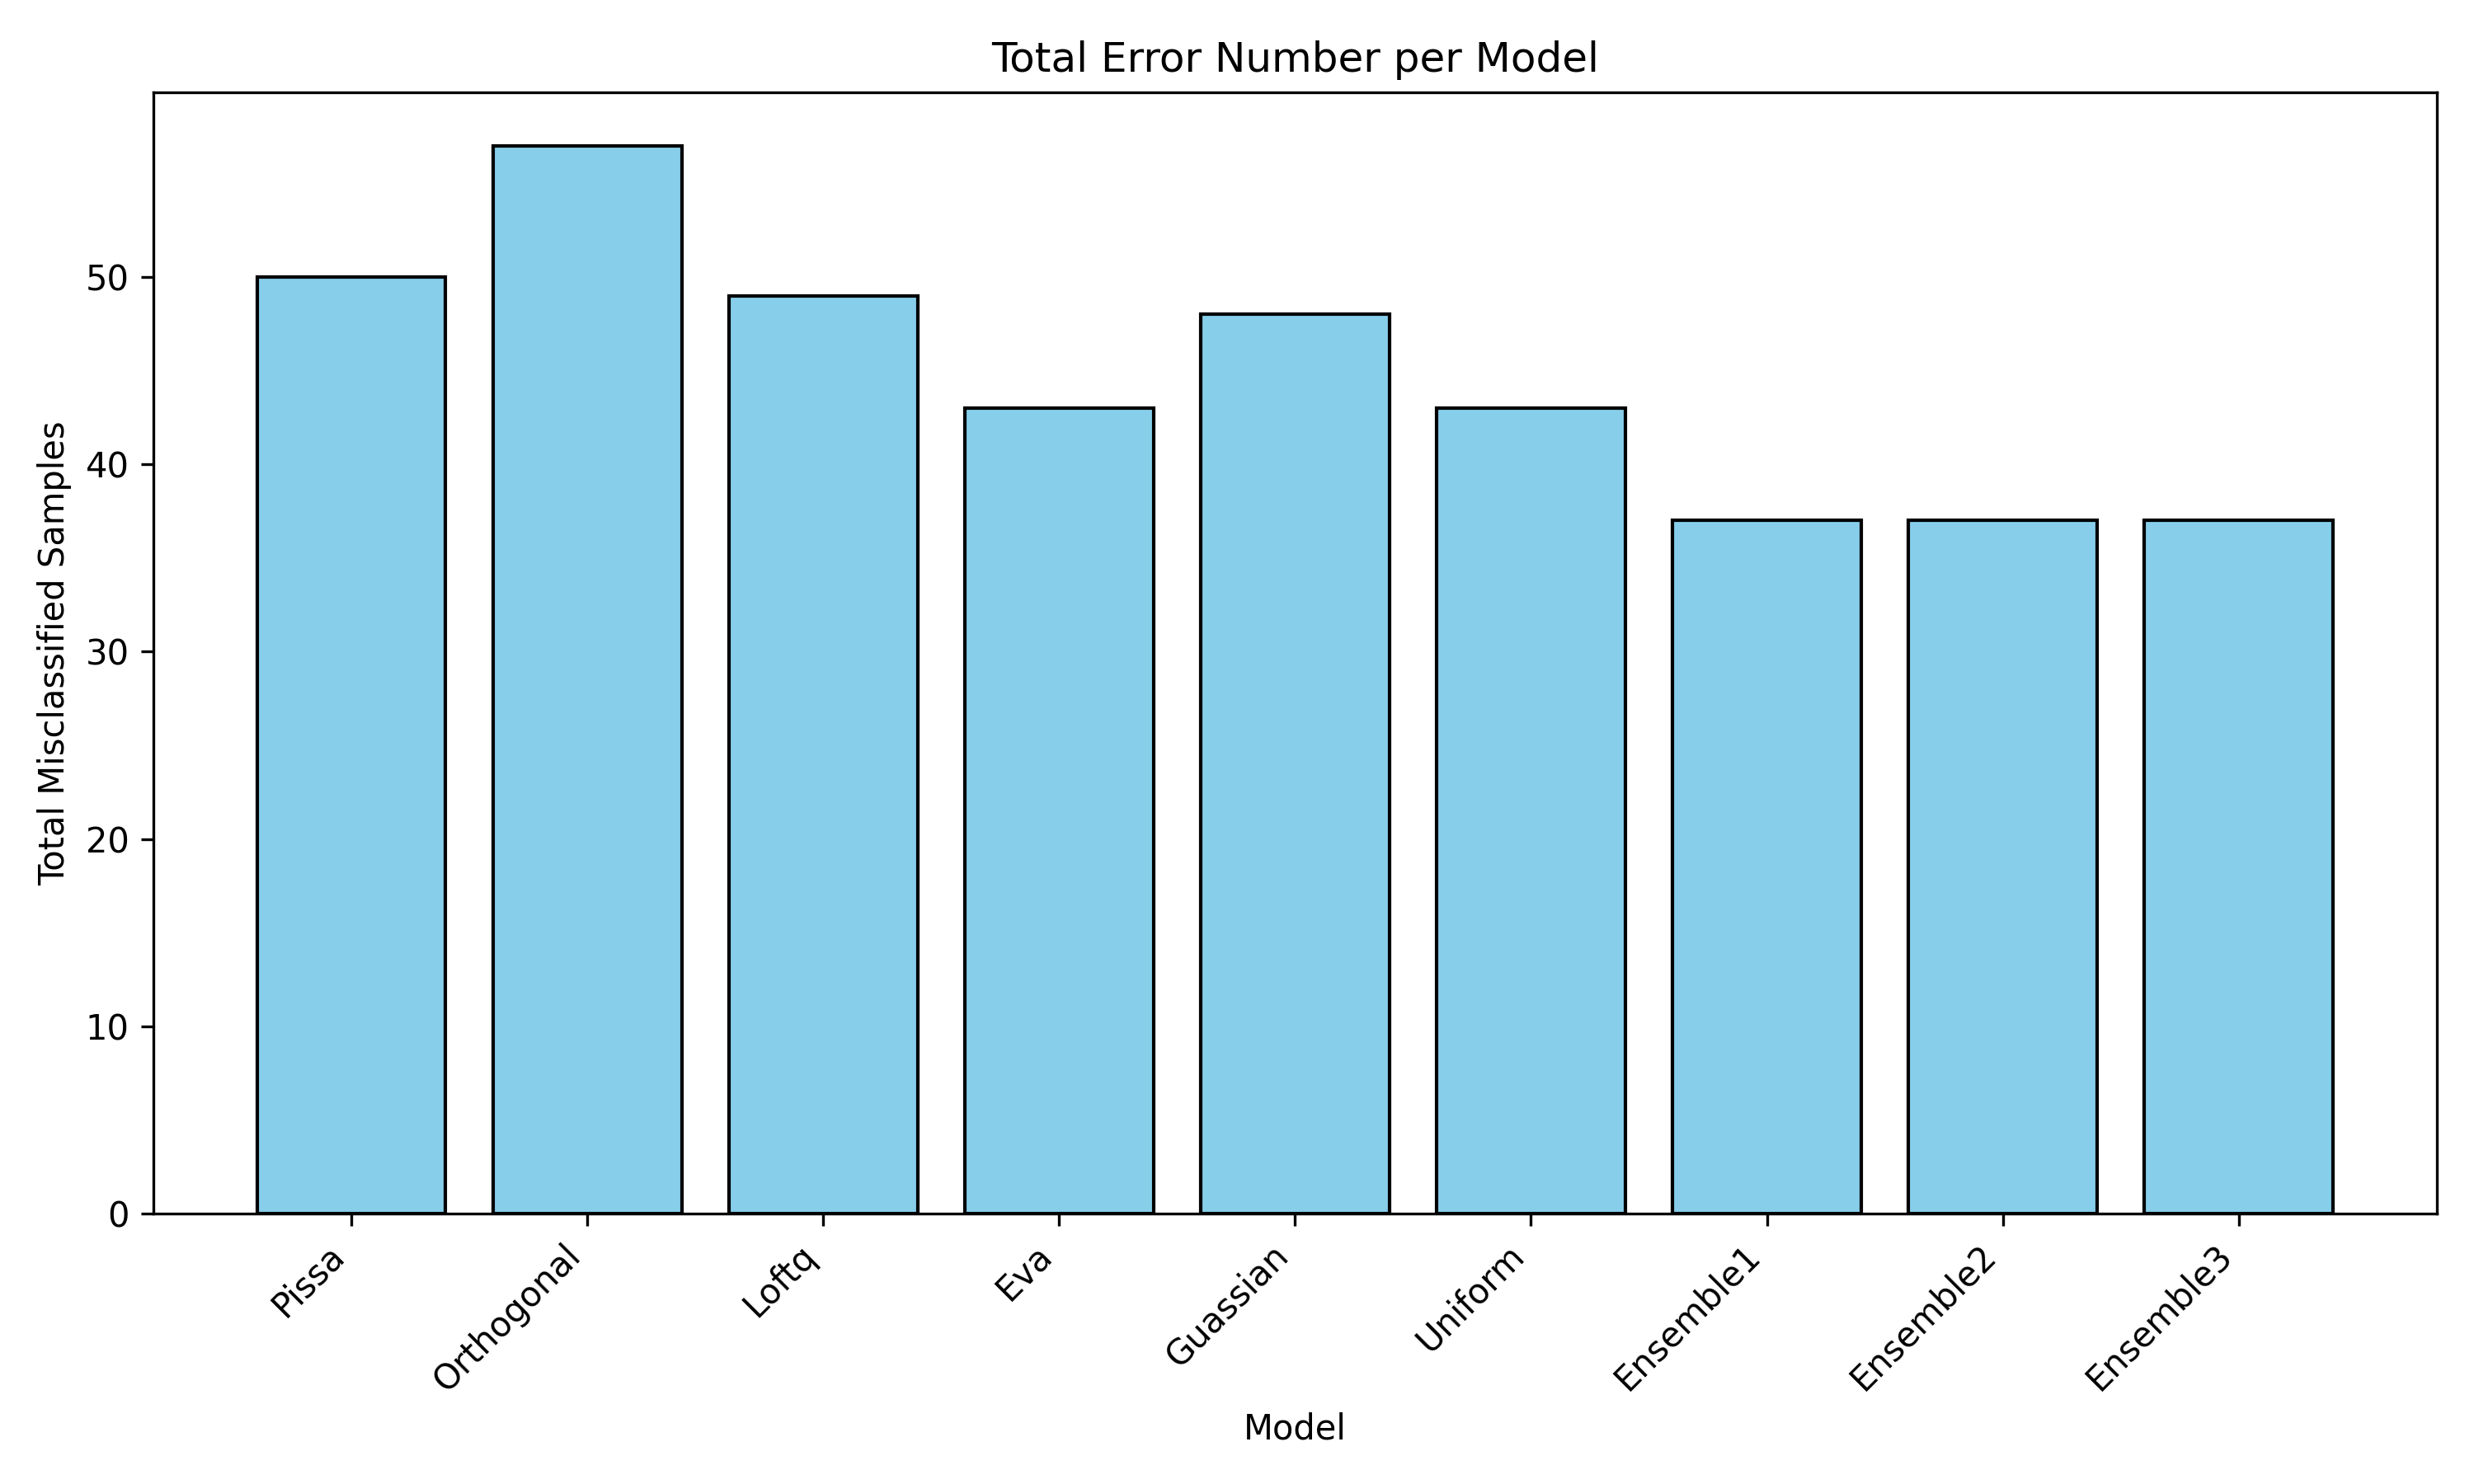
\includegraphics[scale=0.6]{images/gnn_total_error_numbers.png}
    \caption{Comparison of the total number of classification errors between individual models and ensemble learning methods.}
    \small
    The reduction in the number of errors in ensemble methods demonstrates the effective utilization of the diversity in textual representations derived from different initializations.
    \label{fig:error_numbers}
\end{figure}

Table \ref{tab:error_rates} illustrates the error rate for each class, and Figure \ref{fig:error_numbers} presents the total number of classification errors for various models. The individual models consist of GNNs trained using embeddings from different initialization strategies. Additionally, the performance of the ensemble learning method in simple averaging mode (Uniform) and the three proposed trainable versions is reported.

Analysis of the results indicates that the trainable ensemble learning methods achieve the lowest or second-lowest error rates in most classes. This suggests that the proposed ensemble framework is capable of effectively combining the complementary information present in the individual models. 

Furthermore, it is observed that the proposed trainable ensemble methods outperform simple averaging in the majority of classes. This indicates that learning the combination coefficients in a data-driven manner can yield better performance compared to a static and uniform aggregation of models.

\subsubsection{Analysis of the Impact of Fine-Tuning on the Quality of Textual Embeddings}

The objective of this experiment is to investigate whether fine-tuning a LLM can yield a statistically significant improvement in downstream performance. To this end, textual embeddings of the graph are extracted in two states:
(1) prior to fine-tuning and
(2) after fine-tuning.

Subsequently, a separate GNN is trained using each set of embeddings. Finally, the two resulting models are evaluated on the same samples in the test set, and their results are compared pairwise.

Since both models are evaluated on identical samples and their outputs are recorded as correct/incorrect for each sample, \textbf{McNemar's Test} is employed for the statistical comparison. This test is suitable for comparing two dependent classifiers.

The statistical hypotheses are defined as follows:
\[
H_0: \text{The error rates of the fine-tuned model and the base model are equal.}
\]
\[
H_1: \text{There is a significant difference between the error rates of the two models.}
\]

\revthree{The McNemar test statistic with Edwards' continuity correction is}
\begin{equation}
\revthree{\chi^2 = \frac{\left(|b - c| - 1\right)^2}{b + c},}
\label{eq:mcnemar}
\end{equation}

where:
\(b\) is the number of samples correctly classified by the base model but incorrectly by the fine-tuned model,
and \(c\) is the number of samples correctly classified by the fine-tuned model but incorrectly by the base model.
\revthree{Under $H_0$ the statistic follows a $\chi^2$ distribution with one degree of freedom. When $b+c<25$, the exact binomial form of the test is used instead.}

In this research, the significance level is set at \(\alpha = 0.05\).
\revthree{Because the same hypothesis is tested on several datasets, the $p$-values are adjusted with the Holm--Bonferroni procedure \citep{holm1979simple} over all comparisons performed. It controls the family-wise error rate at $\alpha=0.05$, like the Bonferroni correction, and rejects at least as often. For transparency, Table~\ref{tab:mcnemar} also reports the Bonferroni-adjusted $p$-values and two effect sizes: the accuracy difference $(c-b)/n$, where $n$ is the number of test nodes, and the discordant ratio $c/b$. All numbers were recomputed so that on each dataset the LoRA adapter, both GNNs (GraphSAGE) and the test use the same 60/20/20 split, so no test node was seen during fine-tuning. The fine-tuned embeddings come from a single LoRA initialization, fixed in advance and identical for all datasets.}

The results of McNemar's test for various datasets are presented in Table \ref{tab:mcnemar}.

\revthree{After the Holm--Bonferroni correction, the fine-tuned embeddings are significantly more accurate than the base embeddings on five of the seven datasets, with gains from $+0.70$ pp (OGBN-ArXiv) to $+9.58$ pp (Computers); all of them except WikiCS also pass the Bonferroni correction. On CiteSeer the fine-tuned embeddings are more accurate as well ($+3.13$ pp, unadjusted $p=0.0126$), but the difference does not survive the correction (adjusted $p=0.0969$). Reddit is the only dataset where fine-tuning does not help: the fine-tuned embeddings are $1.27$ pp less accurate, and the difference is not significant after the correction (adjusted $p=0.0969$). On this dataset the label (popular vs.\ normal user) is only weakly reflected in the text of the posts: the base embeddings reach only $64.9\%$ on this balanced binary task, so adapting the encoder to the text has little to gain. Fine-tuning the LLM therefore improves the downstream GNN whenever the node text carries the label signal. The gain of DIVERGE itself, which combines the five views, is tested in Section~\ref{sec:significance_baselines}.}

\subsubsection{\revcommon{Computational Cost and Parallel Execution}}\label{sec:efficiency}

\revcommon[R1,R2,R4]{Training the LLM once per LoRA initialization multiplies the fine-tuning cost by the number of runs $M$. DIVERGE keeps this cost manageable in two ways. First, it uses small LLMs with fewer than two billion parameters and trains only LoRA adapters. One run needs 3.9--7.3 GB of GPU memory and adds only 6.5--12.2 MB of adapter weights, so all five views share one base model and fit on a single consumer GPU. Table~\ref{tab:cost} shows that LLM fine-tuning is the dominant cost, while embedding extraction, GNN training and the ensemble head are comparatively cheap.}

\revcommon[R1,R2,R4]{Second, the $M$ runs are independent of each other, so DIVERGE executes them in parallel on the same GPU instead of one after another. Since a small LLM occupies only part of the GPU memory, several runs, and later the corresponding GNNs, fit on the device at once. Table~\ref{tab:parallel} compares sequential and parallel execution. On a 24 GB GPU, two to four runs fit together and the full pipeline finishes $1.41$--$2.02\times$ faster; on a 12 GB GPU, the smallest encoder (LLaMA-3.2-1B) still runs two views at once ($1.41\times$). The smaller the LLM, the more views run in parallel and the larger the saving.}

\revcommon[R1,R2,R4]{DIVERGE still costs more than a single LoRA run, and it replaces an API bill (Table~\ref{tab:api_cost}) with local GPU time. The trade-off is least favourable on ArXiv, where five runs take about 22--26 GPU-hours and the learned ensemble adds only about 0.3 points over uniform averaging (78.11 vs.\ 77.80 with LLaMA-3.2-1B, and $+0.31$ with the other two encoders; Table~\ref{tab:diverge_llm_encoders}), because the views are strong and largely agree. For very large graphs, fewer runs (Table~\ref{tab:diverge_num_finetuned_llms}) are therefore the cost-effective choice.}

\subsubsection{\revone{Analysis of API Cost}}\label{sec:api_cost}

\revone{Table~\ref{tab:api_cost} estimates what the augmentation step of three augmentation-based methods, TAPE \citep{he2024harnessing}, UltraTAG \citep{yu2025ultratag} and E-LLaGNN \citep{Jaiswal2024AllAgainstSome}, would cost with GPT-4o. Input tokens are counted with the GPT-4o tokenizer on the actual node texts and prompts, and output lengths are taken from the GPT-4o explanations we generated for TAPE. TAPE queries every node; UltraTAG queries every node for text augmentation and every edge between its PageRank-selected important nodes (top 10\% of training nodes); E-LLaGNN uses its best reported budget (25\% of nodes, or 10{,}000 nodes on ArXiv). The estimates are lower bounds, since they exclude retries, prompt tuning and E-LLaGNN's repeated per-epoch augmentation.The same procedure reproduces the 128 USD that \citet{he2024harnessing} report for ogbn-arxiv with GPT-3.5. The cost grows linearly with graph size: a single augmentation pass on ArXiv costs about 400 USD for TAPE and UltraTAG, and it must be paid again whenever nodes are added or prompts change. E-LLaGNN is cheaper because it augments only a subset of nodes, but it still needs 10{,}000 API calls on ArXiv. DIVERGE makes no API calls and uses only the native node text, yet it is more accurate than all three augmentation-based methods on all seven benchmarks (Tables~\ref{tab:diverge_node_classification_accuracy_sota} and~\ref{tab:diverge_node_classification_macro_f1_sota}), for example 78.11\% versus 75.92\% for TAPE on ArXiv. Avoiding API fees does not, however, mean lower computation: DIVERGE spends local GPU time instead, which we report in Section~\ref{sec:efficiency}.}

\subsubsection{\revone{Privacy and Security Considerations}}\label{sec:privacy}

\revone{DIVERGE removes one specific risk: node text is never sent to an external LLM provider, where it could be logged, retained or reused, and it stays under the operator's own data-residency and access rules. Local deployment is, however, not a formal privacy guarantee. The pipeline writes new artifacts to disk that still carry information about the text (Table~\ref{tab:privacy_artifacts}). Fine-tuned models can memorize their training text \citep{carlini2021extracting}, and dense text embeddings can be inverted to recover words or even whole sentences \citep{song2020information, morris2023text}. An insider or attacker who obtains these artifacts is outside what local deployment protects against. Embeddings and adapters should therefore be governed like the raw corpus: access control, encryption at rest and audit logs; base weights verified by checksum and loaded as \texttt{safetensors}; pinned library versions; and offline execution without hub access or telemetry. Removing a node on request is not complete when only its embedding is deleted, because the adapters and GNNs trained on it must also be retrained.}

\revone{To measure how much text leaks through the saved embeddings, we ran a keyword-inference attack on Cora and CiteSeer, on each of the four splits (seeds 42--45) with the adapters fine-tuned on that split. For each of the 100 most frequent content words, a linear probe is trained on the training nodes to predict from a node's embedding whether the word occurs in its text. We report the mean test ROC-AUC, where $0.5$ means no leakage. As a reference, the same probe given only the class label reaches $0.58$ on both datasets. Table~\ref{tab:privacy_probe} shows that every embedding set leaks well beyond the label. The AUC of the LoRA embeddings is $0.78$--$0.81$ on Cora and $0.69$--$0.80$ on CiteSeer; the lowest CiteSeer value comes from the Orthogonal adapter, which collapsed on two of the four splits. Fine-tuning lowers leakage compared with the frozen base model ($0.83$ and $0.82$) but does not remove it. Adding Gaussian noise to the stored embeddings reduces leakage only gradually. With noise twice the per-dimension standard deviation ($\sigma=2$), the AUC is still $0.71$ and $0.68$, while GraphSAGE accuracy drops by $0.5$ and $0.3$ points. Simple perturbation is therefore not a sufficient defense. Saved embeddings should not be released and should be deleted once the GNNs are trained. Formal protection requires differentially private training \citep{abadi2016deep}, which we leave to future work.}

\section{Discussion}\label{sec:Discussion}

This section interprets the experimental evidence, states the theoretical and practical implications of DIVERGE, and clarifies how the proposed framework differs from representative prior TAG methods summarized in Table~\ref{tab:related_gap}.

\subsection{Interpretation of main findings}\label{sec:resultsAnalysis}

The results in Tables~\ref{tab:diverge_node_classification_accuracy_sota} and~\ref{tab:diverge_node_classification_macro_f1_sota} support a single overarching claim: \emph{representation diversity induced by LoRA initialization, rather than textual augmentation, is sufficient to outperform augmentation-heavy LLM--GNN pipelines when node texts are already informative}. \revcommon[R2,R4]{Across the seven benchmarks, DIVERGE achieves the best accuracy on six and the best Macro-F1 on all seven, among classical GNNs, frozen- and fine-tuned-language-model encoders, augmentation-based enhancers (TAPE, E-LLaGNN, UltraTAG), recent encoder and aggregation methods (STAGE, LLM-BP, SKETCH) and LLM predictors (GraphGPT, LLaGA). Relative to the strongest augmentation-based baseline (TAPE), DIVERGE improves accuracy by 0.32--2.19 percentage points, and relative to the strongest recent baseline (STAGE) by 0.76--3.84 points. The margins are smallest on Cora and Reddit and largest on CiteSeer and OGBN-ArXiv. The exception is Reddit, where the predictor method LLaGA is more accurate (71.06\% vs.\ 65.68\%), although DIVERGE still has the higher Macro-F1. With a GCN instead of a GraphSAGE backbone, DIVERGE reaches $72.63\%$ on Reddit and also exceeds LLaGA (Section~\ref{sec:gnn_encoders}), so the best GNN encoder depends on the graph.}

Three mechanisms explain these improvements. First, different LoRA initialization strategies produce distinct node embeddings despite identical training texts and labels. \revcommon[R1,R2]{The initialization places each adapter in a different and stable region of the weight spectrum, and this difference propagates to the embeddings and predictions, adding significant diversity on top of training randomness (Section~\ref{sec:initDiversity}).} The heterogeneous per-class error profiles in Table~\ref{tab:error_rates} show that the resulting GNN pool is diverse rather than redundant. Second, \revcommon[R1,R2,R4]{the trainable ensemble heads use this diversity safely: when the views are balanced they perform on par with uniform averaging, and when one view is weak, as when an initialization collapses, they down-weight it and clearly improve over averaging (Section~\ref{sec:ensemble_weight_analysis}).} Third, \revthree{LLM fine-tuning itself yields statistically significant downstream gains on five of seven datasets (McNemar's test with Holm correction, Table~\ref{tab:mcnemar}), indicating that the encoder stage materially improves GNN inputs rather than merely recombining fixed representations. The exception is Reddit, where the text carries little of the label signal and fine-tuning does not help.}

Together, these findings answer the motivating question posed in Section~\ref{sec:Preliminaries}: competitive performance \emph{can} be achieved without textual augmentation when diversity is induced directly from native node texts through multiple parameter-efficient fine-tuning trajectories and adaptively ensembled GNN predictions.

\subsection{Theoretical implications}

From a theoretical standpoint, DIVERGE advances TAG research in three ways.

\textbf{Diversity from optimization trajectories.} Most LLM--GNN pipelines derive diversity from different \emph{modalities} or pipeline stages---for example, augmented versus native text (TAPE), retrieved versus local context (SKETCH), or task-adaptive prompting (LLM-BP). DIVERGE instead treats \textbf{LoRA initialization diversity} as a controllable source of complementary semantic subspaces for the same backbone encoder. This extends parameter-efficient fine-tuning theory \citep{Hu2021LoRA, meng2024pissa, paischer2024eva} to graph learning and shows that multiple low-rank adaptation trajectories can explore distinct local minima even under identical node texts and labels. \revcommon[R1,R2,R4]{Our analysis makes this concrete: the initialization decides which subspace of the pretrained weights each adapter modifies, this choice is stable across seeds, and, when training randomness is isolated, it moves the adapters, embeddings and predictions further apart than a change of seed, significantly so in weight space and in the local neighbourhoods of the embeddings (Section~\ref{sec:initQ2}). Downstream, however, the GNNs propagate over the same graph and compress this diversity, so the views disagree on only about a tenth of the nodes.}

\textbf{Limits of textual augmentation.} The preliminaries in Section~\ref{sec:Preliminaries} and the Cora feature comparison in Table~\ref{tab:gnn_features_comparison} demonstrate that LLM-generated augmentations can \emph{degrade} performance when native texts are already rich. DIVERGE provides empirical confirmation at scale: it surpasses TAPE on all \revthree{seven} benchmarks without generating explanations, summaries, or pseudo-labels. Theoretically, this suggests that augmentation should be treated as a conditional strategy---beneficial when texts are sparse or noisy, but potentially harmful when native semantics are sufficient---rather than as a default prerequisite for LLM--GNN integration.

\textbf{Adaptive aggregation over heterogeneous learners.} Uniform logit averaging assumes equal utility across models and classes, an assumption violated when different initializations specialize on different label groups (Table~\ref{tab:error_rates}). DIVERGE's learned model- and class-level weights formalize a more flexible fusion principle: ensemble coefficients should be data-dependent and class-aware. This aligns with broader ensemble-learning theory while offering a concrete, trainable alternative to fixed averaging in TAG pipelines. \revcommon[R1,R2,R4]{Our experiments add an important qualification: the benefit comes from the softmax constraint as much as from the learned weights. An unconstrained combiner overfits the few labelled nodes available for fusion, whereas convex weights reduce to near-uniform weights on balanced pools and remove a failed view on unbalanced ones (Section~\ref{sec:ensemble_weight_analysis}).}

Finally, the results corroborate the LLMNodeBed finding that strong \emph{local} encoders are often more reliable than costly enhancers \citep{Wu2025LLMNode}. DIVERGE operationalizes this insight by investing compute in diverse encoder trajectories rather than in external API-based text generation.

\subsection{Positioning relative to prior work}

Table~\ref{tab:related_gap} summarizes the design differences; here we connect those differences to the empirical outcomes reported in Section~\ref{sec:Results}. \revcommon[R2,R4]{All methods discussed below are included in Tables~\ref{tab:diverge_node_classification_accuracy_sota} and~\ref{tab:diverge_node_classification_macro_f1_sota} and were run under the same splits, seeds and LLM encoder as DIVERGE, so every comparison in this subsection refers to these tables. Margins are given in accuracy percentage points.}

\textbf{Versus TAPE} \citep{he2024harnessing}: TAPE enriches node text via LLM explanations and zero-shot predictions, then uniformly averages multiple GNNs. DIVERGE uses native text only, induces diversity through multi-initialization LoRA, and learns ensemble weights. DIVERGE outperforms TAPE on every benchmark \revcommon[R2,R4]{($+0.32$ to $+2.19$)} despite omitting augmentation and API calls, supporting the claim that initialization-driven diversity can substitute for generated text when node descriptions are informative. \revcommon[R2,R4]{The margins are modest, however, which shows that TAPE's augmented views are a strong source of diversity as well; DIVERGE reaches a similar effect without the API cost (Section~\ref{sec:api_cost}).}

\textbf{Versus STAGE} \citep{zolnai-lucas-etal-2024-stage}: STAGE ensembles GNNs trained on embeddings from a \emph{single} frozen LLM. \revcommon[R2,R4]{It is therefore the closest design to DIVERGE and the most direct test of our two additions: several adapted encoders instead of one frozen encoder, and learned instead of uniform combination weights. DIVERGE is more accurate than STAGE on all seven benchmarks ($+0.76$ to $+3.84$), with the largest gains on OGBN-ArXiv and CiteSeer, and it also has the higher Macro-F1 everywhere. STAGE is cheaper, since it never fine-tunes the LLM, so the comparison quantifies the accuracy that DIVERGE buys with its additional GPU time (Section~\ref{sec:efficiency}).}

\textbf{Versus UltraTAG} \citep{yu2025ultratag}: UltraTAG modularizes augmentation, encoding, and training into a configurable pipeline that may still rely on optional external services. DIVERGE offers a narrower but more deployable encoder--ensemble design with a single diversity mechanism (LoRA initialization) and no augmentation module. \revcommon[R2,R4]{It is more accurate than UltraTAG on all seven benchmarks ($+2.72$ to $+6.12$), which suggests that, on these datasets, augmenting both text and structure adds less than diversifying the encoder of the native text.}

\textbf{Versus LLM-BP} \citep{wang2025llmbp}: LLM-BP introduces diversity through task-adaptive prompting and fuses information via belief propagation on a single embedding space. DIVERGE derives diversity from multiple fine-tuning trajectories of one backbone and fuses GNN logits through learned ensemble weights. The two approaches are complementary in philosophy---graph-adaptive propagation versus heterogeneous-model ensembling. \revcommon[R2,R4]{In our supervised setting DIVERGE is clearly more accurate ($+5.58$ to $+10.69$). We note that LLM-BP is designed for generalization across graphs with few or no labels, so a fully supervised 60/20/20 split does not play to its strengths; the comparison shows what supervised multi-view fine-tuning adds when labels are available, not that LLM-BP is weak in its intended setting.}

\textbf{Versus SKETCH} \citep{zhou-etal-2025sketch}: SKETCH retrieves related texts and distant structural contexts to enrich LM inputs and reduces reliance on conventional GNN propagation. DIVERGE stays GNN-centric and uses only each node's native text, offering a complementary design point: diversity from encoder initialization rather than from retrieved cross-node context. \revcommon[R2,R4]{DIVERGE is more accurate on all seven benchmarks ($+3.63$ to $+7.99$).} Both methods avoid paid API augmentation, but DIVERGE targets settings where local node text is informative and graph propagation through GNNs remains desirable.

\revcommon[R2,R4]{\textbf{Versus E-LLaGNN} \citep{Jaiswal2024AllAgainstSome}: E-LLaGNN lowers the cost of augmentation by enriching only a selected subset of nodes. DIVERGE avoids augmentation entirely and is more accurate on all seven benchmarks ($+2.93$ to $+6.78$).}

\revcommon[R2,R4]{\textbf{Versus LLM predictors.} The only method that outperforms DIVERGE on any benchmark is LLaGA \citep{Chen2024LLaGA} on Reddit ($71.06\%$ vs.\ $65.68\%$ in accuracy, although DIVERGE has the higher Macro-F1). LLaGA instruction-tunes a 7B-parameter LLM, so this gain comes at a much higher computational cost. When the GNN pool of DIVERGE uses GCN instead of GraphSAGE, it is more accurate than LLaGA on Reddit as well ($72.63\%$, Table~\ref{tab:diverge_gnn_encoders}), with a 1B encoder.}

In summary, no prior TAG method simultaneously (i)~induces representation diversity through multi-initialization LoRA on native node text, (ii)~trains a pool of GNNs on complementary embeddings, and (iii)~fuses predictions with learned model- and class-level weights---all without textual augmentation or external APIs. DIVERGE fills this gap empirically on \revthree{seven benchmarks from five domains} and conceptually by reframing diversity as an encoder-side, initialization-driven property rather than an augmentation-side artifact.


\section{Limitations}\label{sec:Limitations}

Despite the strong performance of the proposed DIVERGE framework, several limitations remain.

First, the proposed method demonstrates stronger performance in fully supervised settings compared to semi-supervised scenarios. The primary reason is that the adaptive ensemble learning framework relies on sufficient labeled data in order to effectively learn the contribution and weighting of different models. In semi-supervised settings, where only a limited number of labeled nodes are available, the ensemble model may not accurately estimate the optimal combination coefficients, which can reduce the overall effectiveness of the framework.

Second, although the proposed approach eliminates the need for costly textual augmentation and external LLM API calls, it does not fully exploit all capabilities of LLMs. In this work, LLMs are mainly utilized as semantic encoders for extracting node-level textual representations. However, recent studies have shown that LLMs can also play important roles as graph enhancers, for example through structural refinement, semantic edge generation, textual augmentation, or label enhancement. These capabilities were not extensively explored in the current framework.

Another limitation is the computational overhead associated with training multiple LLMs and GNNs using different initialization strategies. \revcommon[R1,R2,R4]{Fine-tuning the LLM once per view multiplies the dominant cost by $M$: with five views, the pipeline takes from 0.8 GPU-hours on Cora to about 22--26 GPU-hours on OGBN-ArXiv on one consumer GPU (Section~\ref{sec:efficiency}). DIVERGE removes API fees but not computation, and frozen-encoder methods such as STAGE are cheaper. Parallel execution shortens the wall-clock time but not the total GPU time, and on ArXiv the learned ensemble adds only about 0.3 points over uniform averaging. Using two or three views recovers most of the gain at a proportionally lower cost.}

\revcommon[R1,R2,R4]{The diversity created by the initialization is compressed along the pipeline. Nearly orthogonal adapters give embeddings with a CKA of about $0.7$, and because all GNNs propagate over the same graph, the views disagree on only about a tenth of the test nodes. In the controlled experiments the initialization is a significantly larger source of diversity than the seed in weight space and in the local neighbourhoods, but for the global embedding geometry and the predictions the effect, although in the same direction in every pool, is mostly not significant with pools of this size. In addition, one initialization (Orthogonal) occasionally collapses during fine-tuning; the learned weights neutralize such a view, but its training cost is wasted.}

\revone{Regarding the domains, the evaluation now includes a social network (Reddit) and an e-commerce graph (Computers) besides citation and hyperlink graphs. On Reddit, where the label is only weakly reflected in the node text, fine-tuning does not improve the embeddings and the GraphSAGE version of DIVERGE is less accurate than the 7B predictor LLaGA; the GCN version is more accurate. The benefit of text-derived diversity is therefore smaller when the text carries little of the label signal. The largest benchmark has 169K nodes, all encoders have fewer than two billion parameters, and the two predictor baselines could not be re-run on our hardware, so their numbers come from a different random assignment of nodes to splits.}

\revone{Finally, local deployment is not a formal privacy guarantee. The saved embeddings still allow a simple probe to infer which words occur in a node's text, adding Gaussian noise reduces this only gradually, and differentially private training was not explored (Section~\ref{sec:privacy}).}

Future work can address these limitations by designing more robust ensemble mechanisms for low-label regimes, integrating structural and textual enhancement capabilities of LLMs, reducing the computational complexity of multi-model training, \revone{adding formal privacy protection such as differentially private fine-tuning,} and extending the framework to \revone{larger graphs and larger LLM encoders}.

\section{Conclusion}\label{sec:Conclusion}

In this paper, we proposed \textbf{DIVERGE}, a novel framework for learning on text-attributed graphs that combines LLMs and GNNs through diverse representation learning and adaptive ensemble mechanisms. Unlike previous approaches that rely heavily on expensive textual augmentation or external LLM APIs, the proposed method demonstrates that diverse and complementary node representations can be effectively generated solely from the original graph texts by utilizing multiple LoRA fine-tuning strategies with different parameter initializations.

To achieve this objective, multiple parameter-efficient LLMs were independently fine-tuned using different initialization methods, and the extracted textual representations were used to train multiple GNNs. Subsequently, an adaptive ensemble learning framework was introduced to combine the outputs of these graph models through trainable weighting mechanisms at both the model and class levels. \revcommon[R1,R2,R4]{Experiments on seven text-attributed graph benchmarks from five domains (Cora, CiteSeer, PubMed, WikiCS, OGBN-ArXiv, Reddit and Computers), with the baselines re-run under the same splits and seeds, showed that DIVERGE achieves the best accuracy on six benchmarks and the best Macro-F1 on all seven. On Reddit, the 7B predictor LLaGA is more accurate than the GraphSAGE version of DIVERGE but not than its GCN version. The gains hold for three LLM encoders and three GNN encoders, and two or three views already provide most of them.}

\revcommon[R1,R2,R4]{Furthermore, the experimental analysis showed why different LoRA initialization strategies produce distinct and complementary embeddings: each initialization adapts a different and stable subspace of the pretrained weights, this difference propagates to the embeddings and predictions, and it adds diversity beyond training randomness; when training randomness is isolated, the initialization is also a larger source of diversity than the seed. The trainable ensemble heads were more accurate than uniform averaging in every encoder--dataset pair. Their softmax constraint keeps them from overfitting: they behave like averaging when the views are balanced and down-weight a view whose fine-tuning has failed.} In addition, statistical analysis using McNemar's test \revthree{with Holm correction} demonstrated that fine-tuning the LLM leads to statistically significant improvements in downstream graph learning performance \revthree{on five of the seven datasets}. \revone{These gains come at the cost of additional local GPU time, which parallel execution and fewer views keep manageable on a single consumer GPU.}

Overall, the findings of this research suggest that representation diversity itself can serve as an effective alternative to costly textual augmentation for improving learning on text-attributed graphs. By relying on locally fine-tuned encoders rather than external LLM APIs, DIVERGE also offers a deployment path for graphs whose node text cannot leave organizational or regulatory boundaries\revone{; because the saved embeddings and adapters can still reveal the text, they must be protected like the raw data (Section~\ref{sec:privacy})}. The proposed framework opens new directions for integrating parameter-efficient LLM fine-tuning, representation diversity, and adaptive ensemble learning in graph-based machine learning systems.



%\printcredits


\section*{Data availability}
Benchmark datasets are available via \citep{Wu2025} (accessed 6 June 2026).
Source code for DIVERGE is publicly available at \url{https://github.com/nimaiparifard/DIVERGE}.
% [dataset] Wu, X. (2025). LLMNodeBed. Hugging Face Datasets. \url{https://huggingface.co/datasets/xxwu/LLMNodeBed/tree/main} (Accessed 6 June 2026).
% \end{thebibliography}

%% Loading bibliography style file
%\bibliographystyle{model1-num-names}
\FloatBarrier

\bibliographystyle{cas-model2-names}

% Loading bibliography database
\bibliography{cas-refs}

\clearpage
\appendix
\section{\revone{Hyperparameters}}\label{app:hyperparams}

\revone{This appendix lists all hyperparameters of DIVERGE. Table~\ref{tab:hyperparams} gives the LLM and LoRA settings of the three LLM encoders and the per-dataset LLM training schedule, Table~\ref{tab:search_space} the search spaces of the GNN encoders and the ensemble heads, and Tables~\ref{tab:gnn_hp_llama}--\ref{tab:gnn_hp_gemma} the GNN hyperparameters selected for every LLM encoder, GNN encoder and dataset.}

\begin{table*}[htbp]
\centering\color{red}
\caption{LLM and LoRA hyperparameters of the three LLM encoders (top) and the per-dataset LLM training schedule (bottom).}
\label{tab:hyperparams}
\small
\begin{tabular*}{\textwidth}{@{\extracolsep{\fill}} lccc @{}}
\toprule
\textbf{Setting} & \textbf{LLaMA-3.2-1B} & \textbf{SmolLM2-1.7B} & \textbf{Gemma-2-2B} \\
\midrule
Parameters / hidden size / layers & 1.24B / 2048 / 16 & 1.71B / 2048 / 24 & 2.61B / 2304 / 26 \\
Loading precision & bfloat16 & 4-bit & 4-bit \\
Trainable LoRA parameters & 1.72M & 3.16M & 3.21M \\
Peak fine-tuning VRAM & 3.9 GB & 4.8 GB & 7.3 GB \\
Embedding caching batch size & 32 & 8 & 4 \\
\midrule
\multicolumn{4}{l}{\textit{Shared by the three encoders}} \\
\midrule
LoRA rank ($r$) / alpha & \multicolumn{3}{c}{8 / 16, rank-stabilized scaling \citep{kalajdzievski2023rslora}} \\
LoRA target modules & \multicolumn{3}{c}{Query, key, value and output projections; classification head fully trained} \\
LoRA dropout & \multicolumn{3}{c}{0.05} \\
LoRA initialization & \multicolumn{3}{c}{Gaussian, Orthogonal, PiSSA, EVA, LoFTQ ($M=5$ runs)} \\
Learning rate / scheduler & \multicolumn{3}{c}{$2\times10^{-4}$, linear decay with 3\% warm-up} \\
Batch size & \multicolumn{3}{c}{16 (per-device batch 1, gradient accumulation 16)} \\
Max sequence length & \multicolumn{3}{c}{512 tokens} \\
Checkpoint selection & \multicolumn{3}{c}{Best validation accuracy} \\
Node embedding & \multicolumn{3}{c}{Mean of the last hidden layer over non-padding tokens} \\
\bottomrule
\end{tabular*}

\vspace{0.8em}
\footnotesize
\setlength{\tabcolsep}{3pt}
\begin{tabular*}{\textwidth}{@{\extracolsep{\fill}} lccccccc @{}}
\toprule
\textbf{Schedule} & \textbf{Cora} & \textbf{CiteSeer} & \textbf{PubMed} & \textbf{OGBN-ArXiv} & \textbf{WikiCS} & \textbf{Reddit} & \textbf{Computers} \\
\midrule
LLM epochs & 3 & 3 & 2 & 1 & 2 & 1 & 1 \\
Validation every (steps) & 50 & 50 & 500 & 10,000 & 500 & 10,000 & 10,000 \\
\bottomrule
\end{tabular*}
\end{table*}

\begin{table}[htbp]
\centering\color{red}
\caption{Search spaces of the GNN encoders and of the ensemble heads. Both are searched by exhaustive grid search on validation accuracy, separately for every LLM encoder, GNN encoder and dataset.}
\label{tab:search_space}
\small
\begin{tabular*}{\columnwidth}{@{\extracolsep{\fill}} ll @{}}
\toprule
\textbf{Hyperparameter} & \textbf{Values} \\
\midrule
\multicolumn{2}{l}{\textit{GNN encoders (GCN, GIN, GraphSAGE): 512 configurations}} \\
\midrule
Learning rate & $\{10^{-2}, 5\times10^{-3}, 10^{-3}, 10^{-4}\}$ \\
Hidden dimension & $\{128, 256, 512, 1024\}$ \\
Layers & $\{2, 3\}$ \\
Dropout & $\{0.0, 0.01, 0.1, 0.5\}$ \\
Weight decay & $\{0.0, 0.01\}$ \\
Batch normalization & \{no, yes\} \\
Training & Adam, max.\ 200 epochs, early stopping (patience 20) \\
Selection & Top 64 configurations re-run with 5 seeds \\
\midrule
\multicolumn{2}{l}{\textit{Ensemble heads: 36 configurations}} \\
\midrule
MLP layers & $\{2, 3\}$ \\
Hidden size & $\{64, 128, 256\}$ \\
Dropout & $\{0.3, 0.5\}$ \\
Learning rate & $\{10^{-4}, 10^{-3}, 10^{-2}\}$ \\
Training & Adam, 200 epochs, epoch chosen on validation \\
\bottomrule
\end{tabular*}
\end{table}

\begin{table*}[htbp]
\centering\color{red}
\caption{Selected GNN hyperparameters with the LLaMA-3.2-1B encoder, per GNN encoder and dataset (grid search on validation accuracy, Table~\ref{tab:search_space}).}
\label{tab:gnn_hp_llama}
\footnotesize
\setlength{\tabcolsep}{3pt}
\begin{tabular*}{\textwidth}{@{\extracolsep{\fill}} lccccccc @{}}
\toprule
\textbf{Hyperparameter} & \textbf{Cora} & \textbf{CiteSeer} & \textbf{PubMed} & \textbf{OGBN-ArXiv} & \textbf{WikiCS} & \textbf{Reddit} & \textbf{Computers} \\
\midrule
\multicolumn{8}{l}{\textit{GCN}} \\
\midrule
Layers & 2 & 3 & 3 & 2 & 2 & 2 & 3 \\
Hidden dim & 1024 & 128 & 256 & 512 & 1024 & 1024 & 128 \\
Learning rate & $1\times10^{-4}$ & $1\times10^{-3}$ & $5\times10^{-3}$ & $1\times10^{-4}$ & 0.01 & 0.01 & $1\times10^{-3}$ \\
Dropout & 0.0 & 0.1 & 0.01 & 0.5 & 0.1 & 0.01 & 0.1 \\
Weight decay & 0.0 & 0.0 & 0.01 & 0.0 & 0.0 & 0.0 & 0.0 \\
Batch norm & yes & no & yes & no & yes & yes & yes \\
\midrule
\multicolumn{8}{l}{\textit{GIN}} \\
\midrule
Layers & 2 & 2 & 2 & 3 & 3 & 2 & 2 \\
Hidden dim & 128 & 128 & 512 & 256 & 128 & 128 & 256 \\
Learning rate & $1\times10^{-3}$ & 0.01 & $1\times10^{-4}$ & $5\times10^{-3}$ & $1\times10^{-4}$ & 0.01 & $1\times10^{-4}$ \\
Dropout & 0.0 & 0.0 & 0.5 & 0.01 & 0.1 & 0.01 & 0.01 \\
Weight decay & 0.0 & 0.0 & 0.01 & 0.0 & 0.01 & 0.01 & 0.0 \\
Batch norm & yes & yes & no & yes & yes & yes & yes \\
\midrule
\multicolumn{8}{l}{\textit{GraphSAGE}} \\
\midrule
Layers & 3 & 3 & 3 & 2 & 3 & 3 & 3 \\
Hidden dim & 256 & 128 & 256 & 128 & 512 & 512 & 1024 \\
Learning rate & $5\times10^{-3}$ & $1\times10^{-3}$ & 0.01 & 0.01 & $1\times10^{-4}$ & $1\times10^{-3}$ & $1\times10^{-4}$ \\
Dropout & 0.5 & 0.5 & 0.5 & 0.1 & 0.1 & 0.0 & 0.5 \\
Weight decay & 0.0 & 0.01 & 0.01 & 0.0 & 0.01 & 0.01 & 0.0 \\
Batch norm & yes & yes & no & yes & yes & yes & yes \\
\bottomrule
\end{tabular*}
\end{table*}
\begin{table*}[htbp]
\centering\color{red}
\caption{Selected GNN hyperparameters with the SmolLM2-1.7B encoder, per GNN encoder and dataset (grid search on validation accuracy, Table~\ref{tab:search_space}).}
\label{tab:gnn_hp_smollm}
\footnotesize
\setlength{\tabcolsep}{3pt}
\begin{tabular*}{\textwidth}{@{\extracolsep{\fill}} lccccccc @{}}
\toprule
\textbf{Hyperparameter} & \textbf{Cora} & \textbf{CiteSeer} & \textbf{PubMed} & \textbf{OGBN-ArXiv} & \textbf{WikiCS} & \textbf{Reddit} & \textbf{Computers} \\
\midrule
\multicolumn{8}{l}{\textit{GCN}} \\
\midrule
Layers & 2 & 3 & 2 & 3 & 2 & 2 & 3 \\
Hidden dim & 512 & 128 & 256 & 1024 & 256 & 1024 & 512 \\
Learning rate & $1\times10^{-3}$ & $1\times10^{-3}$ & 0.01 & $5\times10^{-3}$ & $1\times10^{-3}$ & 0.01 & $1\times10^{-3}$ \\
Dropout & 0.1 & 0.1 & 0.0 & 0.5 & 0.1 & 0.1 & 0.5 \\
Weight decay & 0.01 & 0.0 & 0.0 & 0.01 & 0.01 & 0.0 & 0.0 \\
Batch norm & no & no & yes & no & yes & yes & yes \\
\midrule
\multicolumn{8}{l}{\textit{GIN}} \\
\midrule
Layers & 2 & 2 & 3 & 2 & 3 & 2 & 2 \\
Hidden dim & 128 & 128 & 256 & 1024 & 128 & 128 & 128 \\
Learning rate & 0.01 & 0.01 & $5\times10^{-3}$ & $1\times10^{-4}$ & $1\times10^{-3}$ & $5\times10^{-3}$ & $1\times10^{-3}$ \\
Dropout & 0.01 & 0.1 & 0.0 & 0.5 & 0.01 & 0.0 & 0.0 \\
Weight decay & 0.0 & 0.0 & 0.01 & 0.0 & 0.0 & 0.0 & 0.0 \\
Batch norm & yes & yes & no & yes & yes & yes & yes \\
\midrule
\multicolumn{8}{l}{\textit{GraphSAGE}} \\
\midrule
Layers & 3 & 3 & 2 & 3 & 2 & 3 & 3 \\
Hidden dim & 128 & 512 & 256 & 128 & 512 & 512 & 512 \\
Learning rate & 0.01 & $1\times10^{-4}$ & $1\times10^{-3}$ & 0.01 & $1\times10^{-4}$ & $1\times10^{-4}$ & $1\times10^{-3}$ \\
Dropout & 0.0 & 0.5 & 0.1 & 0.01 & 0.0 & 0.1 & 0.1 \\
Weight decay & 0.01 & 0.01 & 0.0 & 0.01 & 0.01 & 0.01 & 0.0 \\
Batch norm & no & no & yes & no & yes & yes & yes \\
\bottomrule
\end{tabular*}
\end{table*}
\begin{table*}[htbp]
\centering\color{red}
\caption{Selected GNN hyperparameters with the Gemma-2-2B encoder, per GNN encoder and dataset (grid search on validation accuracy, Table~\ref{tab:search_space}).}
\label{tab:gnn_hp_gemma}
\footnotesize
\setlength{\tabcolsep}{3pt}
\begin{tabular*}{\textwidth}{@{\extracolsep{\fill}} lccccccc @{}}
\toprule
\textbf{Hyperparameter} & \textbf{Cora} & \textbf{CiteSeer} & \textbf{PubMed} & \textbf{OGBN-ArXiv} & \textbf{WikiCS} & \textbf{Reddit} & \textbf{Computers} \\
\midrule
\multicolumn{8}{l}{\textit{GCN}} \\
\midrule
Layers & 2 & 2 & 3 & 2 & 2 & 3 & 2 \\
Hidden dim & 128 & 128 & 512 & 256 & 512 & 128 & 1024 \\
Learning rate & $1\times10^{-3}$ & $5\times10^{-3}$ & $1\times10^{-4}$ & 0.01 & $5\times10^{-3}$ & $5\times10^{-3}$ & $1\times10^{-3}$ \\
Dropout & 0.5 & 0.0 & 0.1 & 0.01 & 0.5 & 0.0 & 0.5 \\
Weight decay & 0.01 & 0.0 & 0.01 & 0.0 & 0.0 & 0.01 & 0.0 \\
Batch norm & yes & yes & no & yes & yes & no & yes \\
\midrule
\multicolumn{8}{l}{\textit{GIN}} \\
\midrule
Layers & 2 & 2 & 2 & 3 & 2 & 2 & 3 \\
Hidden dim & 512 & 512 & 128 & 512 & 256 & 256 & 1024 \\
Learning rate & $1\times10^{-3}$ & $5\times10^{-3}$ & 0.01 & $1\times10^{-3}$ & $1\times10^{-4}$ & $1\times10^{-4}$ & $5\times10^{-3}$ \\
Dropout & 0.0 & 0.01 & 0.5 & 0.0 & 0.0 & 0.01 & 0.1 \\
Weight decay & 0.0 & 0.0 & 0.0 & 0.01 & 0.0 & 0.0 & 0.01 \\
Batch norm & yes & yes & no & yes & yes & no & yes \\
\midrule
\multicolumn{8}{l}{\textit{GraphSAGE}} \\
\midrule
Layers & 3 & 2 & 3 & 2 & 3 & 3 & 2 \\
Hidden dim & 128 & 128 & 512 & 256 & 256 & 128 & 1024 \\
Learning rate & $1\times10^{-3}$ & $1\times10^{-4}$ & $5\times10^{-3}$ & $1\times10^{-3}$ & $1\times10^{-3}$ & 0.01 & $1\times10^{-4}$ \\
Dropout & 0.5 & 0.5 & 0.01 & 0.0 & 0.5 & 0.1 & 0.5 \\
Weight decay & 0.0 & 0.01 & 0.0 & 0.01 & 0.0 & 0.0 & 0.01 \\
Batch norm & yes & no & yes & no & yes & yes & no \\
\bottomrule
\end{tabular*}
\end{table*}

\clearpage
\section{Ablation Study Tables}\label{app:ablation_tables}

This appendix collects the tables of the ablation study (Section~\ref{sec:Results}).

\begin{table}[ht]
\centering
\caption{Comparison of error rates per class for the Cora dataset.}
\label{tab:error_rates}

\begin{tabular*}{\textwidth}{@{\extracolsep{\fill}} lccccccc @{}}
\toprule
\multirow{2}{*}{\textbf{Model}} & \multicolumn{7}{c}{\textbf{Error Rate per Class (\%)}} \\
\cmidrule(lr){2-8}
 & \textbf{Class 0} & \textbf{Class 1} & \textbf{Class 2} & \textbf{Class 3} & \textbf{Class 4} & \textbf{Class 5} & \textbf{Class 6} \\
\midrule

PiSSA      & 44.44 & 2.58 & \textbf{2.78} & 1.20 & 22.39 & 7.89 & 9.89 \\
Orthogonal & 38.89 & 2.58 & 18.06 & 2.41 & 13.43 & 7.89 & 13.19 \\
LoFTQ      & 33.33 & 2.58 & 8.33 & 1.20 & 16.42 & 7.89 & 13.19 \\
EVA        & 25.00 & \textbf{1.29} & 8.33 & 1.20 & 16.42 & 7.89 & 12.09 \\
Gaussian   & 22.22 & 2.58 & 15.28 & 2.41 & 11.94 & 7.89 & 13.19 \\
\midrule
Uniform    & \textbf{13.89} & 3.87 & 12.50 & 1.20 & \textbf{13.43} & 7.89 & 10.99 \\
\midrule
Ensemble1  & \textbf{13.89} & \textbf{1.94} & 8.33 & 1.20 & 16.42 & \textbf{7.89} & \textbf{8.79} \\
Ensemble2  & 19.44 & 2.58 & \textbf{6.94} & \textbf{0.00} & 14.93 & \textbf{7.89} & \textbf{8.79} \\
Ensemble3  & 19.44 & 2.58 & \textbf{6.94} & 1.20 & \textbf{13.43} & \textbf{7.89} & \textbf{8.79} \\
\bottomrule
\end{tabular*}
\end{table}

\begin{table}[h]
\caption{McNemar's test between GNNs on embeddings from the base and the fine-tuned LLM; $b$ and $c$ are the discordant pairs. \revthree{The statistic is continuity-corrected (Eq.~\ref{eq:mcnemar}); $p$-values are adjusted for all comparisons.}}
\label{tab:mcnemar}
\small
\setlength{\tabcolsep}{3pt}
\begin{tabular*}{\textwidth}{@{\extracolsep{\fill}} lccccccc @{}}
\toprule
\textbf{Metric} & \textbf{Cora} & \textbf{CiteSeer} & \textbf{PubMed} & \textbf{WikiCS} & \revthree{\textbf{ArXiv}} & \revthree{\textbf{Computers}} & \revthree{\textbf{Reddit}} \\
\midrule
Both Correct & \revthree{449} & \revthree{472} & \revthree{3511} & \revthree{1964} & \revthree{25010} & \revthree{13781} & \revthree{3734} \\
Base Model Only Correct ($b$) & \revthree{10} & \revthree{19} & \revthree{54} & \revthree{70} & \revthree{1070} & \revthree{372} & \revthree{603} \\
Finetuned Only Correct ($c$) & \revthree{33} & \revthree{39} & \revthree{238} & \revthree{108} & \revthree{1308} & \revthree{2044} & \revthree{518} \\
Both Wrong & \revthree{50} & \revthree{108} & \revthree{141} & \revthree{199} & \revthree{6481} & \revthree{1249} & \revthree{1832} \\
Discordant Pairs ($b+c$) & \revthree{43} & \revthree{58} & \revthree{292} & \revthree{178} & \revthree{2378} & \revthree{2416} & \revthree{1121} \\
McNemar Statistic & \revthree{$11.256$} & \revthree{$6.224$} & \revthree{$114.688$} & \revthree{$7.691$} & \revthree{$23.620$} & \revthree{$1155.729$} & \revthree{$6.294$} \\
$p$-value & \revthree{$7.94\times10^{-4}$} & \revthree{$0.0126$} & \revthree{$9.21\times10^{-27}$} & \revthree{$0.0056$} & \revthree{$1.17\times10^{-6}$} & \revthree{$2.55\times10^{-253}$} & \revthree{$0.0121$} \\
\revthree{Bonferroni-adjusted $p$} & \revthree{$0.0103$} & \revthree{$0.164$} & \revthree{$1.20\times10^{-25}$} & \revthree{$0.0721$} & \revthree{$1.53\times10^{-5}$} & \revthree{$3.32\times10^{-252}$} & \revthree{$0.157$} \\
\revthree{Holm-adjusted $p$} & \revthree{$0.0079$} & \revthree{$0.0969$} & \revthree{$1.11\times10^{-25}$} & \revthree{$0.0499$} & \revthree{$1.29\times10^{-5}$} & \revthree{$3.32\times10^{-252}$} & \revthree{$0.0969$} \\
\revthree{Accuracy difference $(c-b)/n$ (pp)} & \revthree{$+4.24$} & \revthree{$+3.13$} & \revthree{$+4.67$} & \revthree{$+1.62$} & \revthree{$+0.70$} & \revthree{$+9.58$} & \revthree{$-1.27$} \\
\revthree{Discordant ratio $c/b$} & \revthree{$3.30$} & \revthree{$2.05$} & \revthree{$4.41$} & \revthree{$1.54$} & \revthree{$1.22$} & \revthree{$5.49$} & \revthree{$0.86$} \\
\midrule
\textbf{Result} \revthree{(Holm)} & \revthree{Reject $H_0$} & \revthree{Fail to reject $H_0$} & \revthree{Reject $H_0$} & \revthree{Reject $H_0$} & \revthree{Reject $H_0$} & \revthree{Reject $H_0$} & \revthree{Fail to reject $H_0$} \\
\bottomrule
\end{tabular*}
\end{table}

\begin{table}[htbp]
\centering\color{revshared}
\caption{DIVERGE (Method~3) against the strongest reported baseline per dataset (two-proportion $z$-test, Holm-adjusted over 70 dataset--baseline pairs), and the number of the 14 baselines it significantly outperforms.}
\label{tab:significance_reported}
\small
\setlength{\tabcolsep}{3pt}
\begin{tabular*}{\textwidth}{@{\extracolsep{\fill}} lccccc @{}}
\toprule
 & \textbf{Cora} & \textbf{CiteSeer} & \textbf{PubMed} & \textbf{WikiCS} & \textbf{ArXiv} \\
\midrule
Test nodes $n$                    & 542 & 638 & 3944 & 2341 & 33869 \\
DIVERGE accuracy (\%)             & 89.94 & 79.50 & 95.23 & 88.59 & 78.01 \\
Strongest baseline                & TAPE & TAPE & TAPE & TAPE & TAPE \\
Its reported accuracy (\%)        & 89.32 & 77.65 & 93.98 & 87.24 & 75.92 \\
Difference (pp)                   & $+0.62$ & $+1.85$ & $+1.25$ & $+1.35$ & $+2.09$ \\
Holm-adjusted $p$                 & 1 & 1 & 0.32 & 1 & $4.98\times10^{-9}$ \\
Baselines significantly below DIVERGE & 4/14 & 2/14 & 12/14 & 8/14 & 14/14 \\
\bottomrule
\end{tabular*}
\end{table}

\begin{table*}[htbp]
\centering\color{revshared}
\caption{Cost of each DIVERGE stage for one PiSSA run on one RTX 5070 (12 GB). Below each backbone: peak fine-tuning memory / adapter size. Last column: full DIVERGE pipeline with the five runs in sequence.}
\label{tab:cost}
\small
\begin{tabular*}{\textwidth}{@{\extracolsep{\fill}} llcccccc @{}}
\toprule
\textbf{Backbone} & & \textbf{FT} & \textbf{Caching} & \textbf{GNN} & \textbf{Ensemble} & \textbf{1 run} & \textbf{DIVERGE} \\
\textbf{(VRAM / adapter)} & \textbf{Dataset} & (min) & (min) & (s) & (s) & (GPU-h) & (GPU-h) \\
\midrule
% Generated by experiments/computational_cost_estimator.py (results/computational_cost/cost_table_rows.tex)
\multirow{5}{*}{\shortstack[l]{LLaMA-3.2-1B\\ 3.9 GB / 6.5 MB}} & Cora & 8.1 & 1.1 & 3.5 & 120 & 0.15 & 0.80 \\
 & CiteSeer & 10.0 & 1.1 & 3.5 & 120 & 0.19 & 0.96 \\
 & PubMed & 91.7 & 7.6 & 5.0 & 121 & 1.66 & 8.32 \\
 & WikiCS & 43.5 & 6.3 & 3.8 & 121 & 0.83 & 4.19 \\
 & ArXiv & 225.1 & 65.0 & 10.1 & 174 & 4.84 & 24.24 \\
\midrule
\multirow{5}{*}{\shortstack[l]{SmolLM2-1.7B\\ 4.8 GB / 12.0 MB}} & Cora & 12.1 & 1.8 & 3.5 & 120 & 0.23 & 1.19 \\
 & CiteSeer & 14.9 & 1.9 & 3.5 & 120 & 0.28 & 1.44 \\
 & PubMed & 65.3 & 14.4 & 5.0 & 121 & 1.33 & 6.69 \\
 & WikiCS & 35.3 & 11.1 & 3.8 & 121 & 0.77 & 3.91 \\
 & ArXiv & 151.5 & 111.7 & 10.1 & 174 & 4.39 & 22.00 \\
\midrule
\multirow{5}{*}{\shortstack[l]{Gemma-2-2B\\ 7.3 GB / 12.2 MB}} & Cora & 15.2 & 2.4 & 3.6 & 120 & 0.29 & 1.50 \\
 & CiteSeer & 18.5 & 2.4 & 3.6 & 120 & 0.35 & 1.78 \\
 & PubMed & 71.5 & 17.4 & 5.2 & 121 & 1.48 & 7.45 \\
 & WikiCS & 39.8 & 14.3 & 3.9 & 121 & 0.90 & 4.55 \\
 & ArXiv & 163.8 & 144.2 & 10.9 & 174 & 5.14 & 25.73 \\
\bottomrule
\end{tabular*}
\end{table*}

\begin{table}[htbp]
\centering\color{revshared}
\caption{Wall-clock hours of the full DIVERGE pipeline (PiSSA, five datasets) with sequential or parallel LoRA runs on one GPU; $k$: runs in parallel. Parallel times are estimated from single-run measurements.}
\label{tab:parallel}
\small
\setlength{\tabcolsep}{3pt}
\begin{tabular*}{\columnwidth}{@{\extracolsep{\fill}} lccccccccc @{}}
\toprule
 & \textbf{VRAM} & \textbf{1 run} & \textbf{Seq.} & \multicolumn{3}{c}{\textbf{12 GB}} & \multicolumn{3}{c}{\textbf{24 GB}} \\
\cmidrule(lr){5-7}\cmidrule(lr){8-10}
\textbf{Backbone} & \textbf{/job} & \textbf{(h)} & \textbf{(h)} & $k$ & \textbf{h} & \textbf{Speed-up} & $k$ & \textbf{h} & \textbf{Speed-up} \\
\midrule
LLaMA-3.2-1B & 4.5 & 7.8 & 38.5 & 2 & 27.3 & 1.41$\times$ & 4 & 19.0 & 2.02$\times$ \\
SmolLM2-1.7B & 5.4 & 7.2 & 35.2 & 1 & 35.2 & 1.00$\times$ & 3 & 18.8 & 1.87$\times$ \\
Gemma-2-2B & 7.9 & 8.3 & 41.0 & 1 & 41.0 & 1.00$\times$ & 2 & 29.0 & 1.41$\times$ \\
\bottomrule
\end{tabular*}
\end{table}

\begin{table}[htbp]
\centering\color{red}
\caption{Estimated API cost (USD) of one LLM augmentation pass with GPT-4o (2.50/10.00 USD per million input/output tokens; the Batch API halves all values). The values are lower bounds (Section~\ref{sec:api_cost}).}
\label{tab:api_cost}
\small
\setlength{\tabcolsep}{3pt}
\begin{tabular*}{\columnwidth}{@{\extracolsep{\fill}} lcccccc @{}}
\toprule
\textbf{Method} & \textbf{Cora} & \textbf{CiteSeer} & \textbf{PubMed} & \textbf{WikiCS} & \textbf{ArXiv} & \textbf{Total} \\
\midrule
% API calls -- TAPE: 2,708 / 3,186 / 19,717 / 11,701 / 169,343
%              UltraTAG: 2,870 / 3,400 / 23,009 / 32,862 / 268,051
%              E-LLaGNN: 677 / 796 / 4,929 / 2,925 / 10,000
% Generated by experiments/api_simulator_calculator.py (results/api_cost/)
TAPE & 4.96 & 6.64 & 53.05 & 32.35 & 398.31 & 495.32 \\
UltraTAG & 3.98 & 4.38 & 30.23 & 31.13 & 403.25 & 472.98 \\
E-LLaGNN & 1.04 & 1.52 & 10.44 & 4.84 & 20.92 & 38.76 \\
\midrule
\textbf{DIVERGE (ours)} & \textbf{0} & \textbf{0} & \textbf{0} & \textbf{0} & \textbf{0} & \textbf{0} \\
\bottomrule
\end{tabular*}
\end{table}

\begin{table}[htbp]
\centering\color{red}
\caption{Artifacts produced by a local DIVERGE deployment, what each can reveal about the node text, and recommended safeguards.}
\label{tab:privacy_artifacts}
\small
\begin{tabular*}{\columnwidth}{@{\extracolsep{\fill}} p{0.24\columnwidth} p{0.33\columnwidth} p{0.35\columnwidth} @{}}
\toprule
\textbf{Artifact} & \textbf{Possible leakage} & \textbf{Safeguard} \\
\midrule
Raw node texts & Full content & Access control, encryption at rest \\
Node embeddings ($\times5$) & Words/attributes via inversion or probing & Do not release; delete after GNN training \\
LoRA adapters ($\times5$) & Memorized text, membership & Treat as sensitive as data; DP fine-tuning \\
GNNs and ensemble head & Membership (weak) & Restrict access \\
Base LLM weights & None (public); supply-chain risk & Checksums, \texttt{safetensors}, offline mode \\
\bottomrule
\end{tabular*}
\end{table}

\begin{table}[htbp]
\centering\color{red}
\caption{Keyword-inference leakage from saved embeddings (LLaMA-3.2-1B; mean over four splits). AUC: linear-probe ROC-AUC for the 100 most frequent words ($0.5$ = none); Acc: GraphSAGE accuracy (\%); $\sigma$: relative noise.}
\label{tab:privacy_probe}
\small
\begin{tabular*}{\columnwidth}{@{\extracolsep{\fill}} lcccc @{}}
\toprule
\multirow{2}{*}{\textbf{Embeddings}} & \multicolumn{2}{c}{\textbf{Cora}} & \multicolumn{2}{c}{\textbf{CiteSeer}} \\
\cmidrule(lr){2-3}\cmidrule(lr){4-5}
 & \textbf{AUC} & \textbf{Acc} & \textbf{AUC} & \textbf{Acc} \\
\midrule
Class label only    & 0.575 & --    & 0.582 & --    \\
Frozen base model   & 0.826 & 87.18 & 0.816 & 76.12 \\
\midrule
LoRA Gaussian       & 0.793 & 88.04 & 0.773 & 77.36 \\
LoRA Orthogonal     & 0.781 & 87.98 & 0.769 & 77.29 \\
LoRA PiSSA          & 0.796 & 89.01 & 0.770 & 77.40 \\
LoRA EVA            & 0.812 & 88.64 & 0.798 & 77.39 \\
LoRA LoftQ          & 0.811 & 88.88 & 0.790 & 77.49 \\
\midrule
LoRA mean, $\sigma=0$   & 0.799 & 88.51 & 0.764 & 71.64 \\
LoRA mean, $\sigma=0.5$ & 0.783 & 88.83 & 0.739 & 71.69 \\
LoRA mean, $\sigma=1$   & 0.757 & 88.80 & 0.716 & 71.68 \\
LoRA mean, $\sigma=2$   & 0.715 & 87.98 & 0.679 & 71.39 \\
\bottomrule
\end{tabular*}
\end{table}

\end{document}

